\documentclass[a4paper,12pt]{article} % тип документа

%  Русский язык
\usepackage{mathtext}               % русский язык в формулах
\usepackage[T2A]{fontenc}			% кодировка
\usepackage[utf8]{inputenc}			% кодировка исходного текста
\usepackage[english,russian]{babel}	% локализация и переносы
\usepackage[a1paper]{geometry}
\geometry{papersize={29.7 cm, 25.0 cm}}

\usepackage{graphicx}               % импорт изображений
\usepackage{wrapfig}                % обтекаемые изображения
\graphicspath{{pictures/}}          % обращение к подкаталогу с изображениями
\usepackage{amsfonts}               % буквы с двойными штрихами
\usepackage{indentfirst}            % indent first
\usepackage{amsmath}                % можно выводить фигурные скобочки -- делать системы уравнений
\usepackage[table,xcdraw]{xcolor}   % таблицы
\usepackage{amsmath,amsfonts,amssymb,amsthm,mathtools} % Математика
\usepackage{wasysym}                % ???
\usepackage{upgreek}                % ???  

\usepackage{gensymb} % degree symbol
\usepackage{mathrsfs}

\usepackage{tikz}
\usetikzlibrary{graphs,graphs.standard}

\usepackage{cancel} % перечеркивания

%% Интервалы
\linespread{1}
\usepackage{multirow}

%% Перенос знаков в формулах (по Львовскому)
\newcommand*{\hm}[1]{#1\nobreak\discretionary{}
	{\hbox{$\mathsurround=0pt #1$}}{}}

%% Русские списки
\usepackage{enumitem}
\makeatletter
\AddEnumerateCounter{\asbuk}{\russian@alph}
\makeatother

% Дополнительная работа с математикой
\usepackage{amsmath,amsfonts,amssymb,amsthm,mathtools} % AMS
\usepackage{icomma} % "Умная" запятая: $0,2$ --- число, $0, 2$ --- перечисление

\usepackage{dsfont}
\usepackage{cancel} % перечеркивания

%%% Свои команды
\DeclareMathOperator{\sgn}{\mathop{sgn}}

%%% Программирование
\usepackage{etoolbox} % логические операторы

%%% Страница
\usepackage{extsizes} % Возможность сделать 14-й шрифт
\usepackage{geometry} % Простой способ задавать поля
\geometry{top=20mm}
\geometry{bottom=20mm}
\geometry{left=20mm}
\geometry{right=20mm}

\usepackage{mathrsfs}

\newcommand{\eqdef}{\stackrel{\mathrm{def}}{=}}
\newcommand{\ryad}{\sum\limits^{\infty}_{k = 0}}

\newcommand{\R}{\mathbb{R}}
\newcommand{\N}{\mathbb{N}}
\newcommand{\series}{\sum\limits_{k=1}^{\infty}}
\newcommand{\useries}{\sum\limits_{k=1}^{\infty} u_k}
\newcommand{\useriesl}{\sum\limits_{k=1}^{\infty} u_k < \infty}
\newcommand{\useriese}{\sum\limits_{k=1}^{\infty} u_k = \infty}
\newcommand{\auseries}{\sum\limits_{k=1}^{\infty} |u_k|}
\newcommand{\auseriesl}{\sum\limits_{k=1}^{\infty} |u_k| < \infty}
\newcommand{\auseriese}{\sum\limits_{k=1}^{\infty} |u_k| = \infty}
\newcommand{\sn}{\sum\limits_{k=1}^{n} u_k}

\renewcommand {\ge}{\geqslant}
\renewcommand {\le}{\leqslant}
\renewcommand {\geq}{\geqslant}
\renewcommand {\leq}{\leqslant}
\renewcommand {\epsilon}{\varepsilon}

\usepackage{titlesec}
\titlelabel{\thetitle.\quad}
%%% Для точек после названий секций

\usepackage{hyperref}
%%% Настройка ссылок
\hypersetup
{
	colorlinks = true,
	linkcolor  = black,
	filecolor  = magenta,
	urlcolor   = blue
}
%%% Конец настройки ссылок


\begin{document}
	
	%=======================================================================================
	
	\begin{titlepage}
		\begin{center}
			\
			\vfill
			
			{\LARGE \textsc{\textbf{Методичка по матАНАЛизу}}}
			
			\vspace{2em}
			
			\vfill
			
			Version 5.0\\
			Долгопрудный, 2022
		\end{center}
	\end{titlepage}
	
	%=======================================================================================

	%БИЛЕТ 1
	%=======================================================================================
	
	\section{Аннотация}
	
	\noindent \textit{Введем понятия:}
	
	\begin{enumerate}
		\item $\mathbb{R}^m$ -- $m$-мерное координатное пространство.
		\item Точка $x = (x_1, x_2, \dots, x_m)$ -- точка $m$-мерного пространства, ~ \\ $x_j \in \mathbb{R}, ~
		j = 1, 2, \dots, m$ -- координата точки.
		\item $x, y \in \mathbb{R}^m$; $\rho_e(x, y) = \sqrt{\sum\limits_{j = 1}^m (x_j - y_j)^2}$ -- расстояние между точками $x$ и $y$.
		\item $\mathbb{E}^m = (\mathbb{R}^m, \rho_e)$ -- $m$-мерное евклидово пространство.
		\item $\mathscr{M} = (M, \rho)$ -- метрическое пространство, где $M \subset \mathbb{R}^m$ -- некоторое множество, $\rho(x, y)$ -- функция, задающая расстояние между точками $x, y$ множества $M$ (метрика).
		\item $B_{\varepsilon}(x_0) = \{x \in \mathbb{E}^m : \rho(x, x_0) < \varepsilon \}$ -- $m$-мерный шар с центром в точке $x_0$ и радиусом $\varepsilon$ (шаровая $\varepsilon$-окресность точки $x_0$).
		\item $\text{П}_{r_1, r_2, \dots r_m}(x_0) = \{ x \in \mathbb{E}^m : |x_j - x_{0j}| < r_j, ~ j = 1, 2, \dots, m \}$ -- $m$-мерный прямоугольник с центром $x_0$ и сторонами $2r_1, 2r_2, \dots, 2r_m$.
		\item $\text{П}_r(x_0) = \{ x \in \mathbb{E}^m : |x_j - x_{0j}| < r \}$ -- $m$-мерный квадрат с центром в точке $x_0$ и стороной $2r$.
	\end{enumerate}
	
	\underline{\textbf{Предложение:}}
	
	\begin{enumerate}
		\item В любую шаровую окрестность можно вписать прямоугольную окрестность.
		\item В любую прямоугольную окрестность можно вписать шаровую окрестность.
	\end{enumerate}
	
	\textbf{Доказательство:} Пусть $B_{\varepsilon}(x_0), ~ \text{П}_{r}(x_0)$ -- шаровая и прямоугольная окрестности точки $x_0$, $r = (r_1, r_2, \dots, r_m)$. Везьмем $\delta = min\{r_1, r_2, \dots, r_m \}$, тогда:
	
	\begin{enumerate}
		\item $\text{П}_{\delta}(x_0) \subset B_{\varepsilon}(x_0), ~~ \delta = \frac{\varepsilon}{\sqrt{m}}$.
		\item $B_{\varepsilon}(x_0) \subset \text{П}_{\delta}(x_0), ~~ \delta = \varepsilon$.\\
	\end{enumerate}
	
	\subsection{Предел последовательности точек в $n$–мерном евклидовом пространстве.}
	
	Обозначим $\mathscr{M} = (M, \rho)$, $\{x^n \}_{n = 1}^{\infty}$ -- последовательность точек в $\mathscr{M}$.\\
	
	\underline{\textbf{Определение:}} Последовательность $\{x^n \} \subset \mathscr{M}$ точек метрического пространства сходится к точке $a \in \mathscr{M}$, если:
	\begin{equation*}
		\lim\limits_{n \to \infty} \rho(x^n, a) = 0
	\end{equation*}
	
	\[ [\lim\limits_{n \to \infty} x^n = a] \eqdef [\forall \varepsilon > 0 ~ \exists N = N(\varepsilon) : \forall n \geqslant N \mapsto \rho(x^n, a) < \varepsilon] \]
	
	\noindent Любой шар с центром в точке $a$ и радиусом $\varepsilon$ содержит все члены последовательности $\{x^n \}$ за исключением быть может конечного числа $N$.\\
	
	\underline{\textbf{Лемма:}} Сходящаяся последовательность точек ограничена.\\
	
	\textbf{Доказательство:}
	
	\[ \lim\limits_{n \to \infty} x^n = a \stackrel{def}{\Rightarrow} \lim\limits_{n \to \infty} y_n = 0 \
	\]
	\noindent где $y_n = \rho(x^n, a)$. Тогда $\{y_n \}$ -- бесконечно малая последовательность $\Rightarrow$ $\{y_n \}$ -- ограничена, т. е. $\exists ~ C > 0 ~ : ~ 0 \leqslant y_n = \rho(x^n, a) \leqslant C$.\\
	
	\underline{\textbf{Лемма:}} Сходящаяся последовательность точек имеет единственный предел.\\
	
	\textbf{Доказательство:} Будем доказывать от противного: предположим, что
	
	\begin{equation*}
		\exists ~ a \neq b : 
		\begin{cases}
			\lim\limits_{n \to \infty} x^n = a\\
			\lim\limits_{n \to \infty} x^n = b
		\end{cases}
		\Rightarrow
	\end{equation*}
	
	\[ (1) ~~ \forall \varepsilon > 0 ~ \exists ~ N_1 = N_1(\varepsilon) : ~ \forall n \geqslant N_1 \mapsto \rho(x^n, a) < \frac{\varepsilon}{2} \]
	
	\[ (2) ~~ \forall \varepsilon > 0 ~ \exists ~ N_2 = N_2(\varepsilon) : ~ \forall n \geqslant N_2 \mapsto \rho(x^n, b) < \frac{\varepsilon}{2} \]
	
	Рассмотрим $N = max \{N_1, N_2\}$, тогда:
	
	\[ \forall \varepsilon > 0 ~ \exists ~ N ~ : ~ \forall n \geqslant N \mapsto \rho(a, b) \leqslant \rho(x^n, a) + \rho(x^n, b) < \varepsilon \]
	
	Таким образом, получаем, что $\rho(a, b) = 0 ~ \Rightarrow ~ a = b$ -- противоречие.\\
	
	\subsection{Теорема Больцано–Вейерштрасса и критерий Коши сходимости последовательности.}
	
	\underline{\textbf{Определение:}} Последовательность точек $\{x^n \} \subset \mathscr{M}$ ограничена, если $\exists R > 0 ~ \forall n \mapsto \rho(x^n, 0) \leqslant R$.\\
	
	\underline{\textbf{Теорема:}} Пусть $\{x^n \} = \{x_1^n, x_2^n, x_3^n, \dots, x_m^n\} \subset \mathbb{E}^m$ -- последовательность точек $m$-мерного евклидового пространства, а $a = (a_1, a_2, \dots, a_m) \in \mathbb{E}^m$ -- точка $m$-мерного евклидового пространства, тогда
	
	\[ x^n \xrightarrow[n \to \infty]{} a ~ \Leftrightarrow ~ \forall j ~ x_j^n \xrightarrow[n \to \infty]{} a_j \]
	
	\textbf{Доказательство:} 
	
	\textit{Необходимость} ($\Rightarrow$)\\
	
	По условию дано:
	
	\[ \forall \varepsilon > 0 ~ \exists N = N(\varepsilon) : ~ \forall n \geqslant N \mapsto \rho(x^n, a) < \varepsilon \]
	
	Тогда:
	
	\[ \rho(x^n, a) = \sqrt{\sum\limits_{j = 1}^m (x_j^n - a_j)^2} \Rightarrow |x_j^n - a_j| \leqslant \rho(x^n, a) < \varepsilon \]
	
	Таким образом получаем:
	
	\[ [\forall \varepsilon > 0 ~ \exists N = N(\varepsilon) : ~ \forall n \geqslant N ~~ \& ~~ \forall j = 1, 2, \dots, m \mapsto |x_j^n - a_j| < \varepsilon] \stackrel{def}{=} \lim\limits_{n \to \infty} x_j^n = a_j \]
	
	\textit{Достаточность} ($\Leftarrow$)\\
	
	Запишем определение покоординатной сходимости:
	
	\[ \forall \varepsilon > 0 ~ \exists ~ N_j = N_j(\varepsilon) : ~ \forall n \geqslant N_j \mapsto |x_j - a_j| < \frac{\varepsilon}{\sqrt{m}} \]
	
	Пусть $N = max\{N_1, N_2, \dots, N_m \} \Rightarrow \forall n \geqslant N \mapsto |x_j - a_j| < \frac{\varepsilon}{\sqrt{m}}$ для всех $j$.
	
	\[ \rho(x^n, a) = \sqrt{\sum\limits_{j = 1}^m (x_j^n - a_j)^2} < \sqrt{m \cdot \frac{\varepsilon^2}{m}} = \varepsilon \Rightarrow \]
	
	\[ \lim\limits_{n \to \infty} x^n = a \]\\
	
	\underline{\textbf{Теорема [Теорема Больцано-Вейерштрасса]:}} Из любой ограниченной последовательности $\{x^n \} \subset \mathbb{E}^m$ можно выделить сходящуюся подпоследовательность $\{x^{k_n} \} \subset \mathbb{E}^m$.\\
	
	\textbf{Доказательство:}
	
	$\{x^n \} \subset \mathbb{E}^m$ является ограниченной $\stackrel{def}{\Rightarrow}$ $\exists R > 0 ~ \forall n \mapsto \rho_e(x^n, 0) \leqslant R$. Тогда для всех $j$ последовательность $\{x_j^n \}$ так же ограничена ($x_j^n$ -- $j$-ая компонента).\\
	
	$\{x_1^n \}$ ограничена, тогда по теореме Больцано-Вейерштраcса для числовой последовательности существует подпоследовательность $\{x_1^{k_{n_1}} \}$ такая, что $x_1^{k_{n_1}} \xrightarrow[n_1 \to \infty]{} a_1$.\\
	
	Возьмём подпоследовательность $\{x^{k_{n_1}} \} \subset \mathbb{E}^m$ (по номерам $k_{n_1}$ выбираем из последовательности $\{x^n \}$ точки). И рассмотрим числовую последовательность $\{x_2^{k_{n_1}} \}$. Она ограничена (как подпоследовательность ограниченной последовательности) и следовательно, по теореме Больцано-Вейерштраса существует подпоследовательность $\{x_2^{k_{n_2}} \}$ такая, что $x_2^{k_{n_2}} \xrightarrow[n_2 \to \infty]{} a_2$. При этом все еще справедливо $x_1^{k_{n_2}} \xrightarrow[n_2 \to \infty]{} a_1$.\\
	
	\begin{equation*}
		\{x^n \} \subset \mathbb{E}^m \Rightarrow \{x_1^n \} \Rightarrow \{x_1^{k_{n_1}} \} \Rightarrow x_1^{k_{n_1}} \xrightarrow[n_1 \to \infty]{} a_1
	\end{equation*}
	
	\begin{equation*}
		\{x^{k_{n_1}} \} \subset \mathbb{E}^m \Rightarrow \{x_2^{k_{n_1}} \} \Rightarrow \{x_2^{k_{n_2}} \} \Rightarrow 
		\begin{cases}
			x_2^{k_{n_2}} \xrightarrow[n_2 \to \infty]{} a_2\\
			x_1^{k_{n_2}} \xrightarrow[n_2 \to \infty]{} a_1
		\end{cases}    
	\end{equation*}
	
	\begin{equation*}
		\{x^{k_{n_2}} \} \subset \mathbb{E}^m \Rightarrow \{x_3^{k_{n_2}} \} \Rightarrow \{x_3^{k_{n_3}} \} \Rightarrow 
		\begin{cases}
			x_3^{k_{n_3}} \xrightarrow[n_3 \to \infty]{} a_3\\
			x_2^{k_{n_3}} \xrightarrow[n_3 \to \infty]{} a_2\\
			x_1^{k_{n_3}} \xrightarrow[n_3 \to \infty]{} a_1
		\end{cases}    
	\end{equation*}
	
	\[ \dots \]
	
	\begin{equation*}
		\{x^{k_{n_{m-1}}} \} \subset \mathbb{E}^m \Rightarrow \{x_m^{k_{n_{m-1}}} \} \Rightarrow \{x_m^{k_{n_m}} \} \Rightarrow 
		\begin{cases}
			x_m^{k_{n_m}} \xrightarrow[n_m \to \infty]{} a_m\\
			\dots \\
			x_1^{k_{n_m}} \xrightarrow[n_m \to \infty]{} a_1
		\end{cases}    
	\end{equation*}
	
	Таким образом мы нашли подпоследовательность $\{x^{k_{n_m}} \} \subset \mathbb{E}^m$ такую, что $x^{k_{n_m}} \xrightarrow[n_m \to \infty]{} a = (a_1, a_2, \dots, a_m)$.\\
	
	\underline{\textbf{Определение:}} Последовательность точек $\{x^n \} \subset \mathscr{M}$ называется \textit{фундаменталной}, если $\forall \varepsilon > 0 ~ \exists N = N(\varepsilon) : ~ \forall n \geqslant N ~ \& ~ \forall k \geqslant N \mapsto \rho(x^n, x^k) < \varepsilon$.\\
	
	\underline{\textbf{Определение:}} Метрическое пространство $\mathscr{M}$, в котором любая фундаментальная последовательность точек $\{x^n \} \subset \mathscr{M}$ является сходящейся, называется \textit{полным}.\\
	
	\underline{\textbf{Теорема [Критерий Коши]:}} для того, чтобы последовательность $\{x^n \} \subset \mathbb{E}^m$ сходилась, необходимо и достаточно, чтобы она была фундаментальной.\\
	
	\textbf{Доказательство:} 
	
	\textit{Необходимость} $(\Rightarrow)$
	
	\[ x^n \xrightarrow[n \to \infty]{} a \Rightarrow \forall \varepsilon > 0 ~ \exists N = N(\varepsilon) : \]
	
	\[ \forall n \geqslant N \mapsto \rho(x^n, a) < \frac{\varepsilon}{2} \]
	\[ \forall k \geqslant N \mapsto \rho(x^k, a) < \frac{\varepsilon}{2} \]
	
	\[ \rho(x^n, x^k) \leqslant \rho(x^n, a) + \rho(x^k, a) < \varepsilon \]
	
	\textit{Достаточность} $(\Leftarrow)$ 
	
	Докажем, что евклидово пространство $\mathbb{E}^m$ является полным, то есть любая фундаментальная последовательность этого пространства является сходящейся.\\
	
	Рассмотрим последовательность $\{x^n \} \subset \mathbb{E}^m$, которая является фундаментальной. Распишем по определению:
	
	$$ \forall \varepsilon > 0 ~ \exists N = N(\varepsilon) : ~ \forall n \geqslant N \And \forall k \geqslant N \longmapsto \rho(x^n, x^k) < \varepsilon $$
	
	Воспользуемся утверждением:
	
	\[ \forall j \longmapsto |x_j^n - x_j^k| \leqslant \rho(x^n, x^k) < \varepsilon \]
	
	Таким образом, получаем, что последовательность $\{ x_j \}$ является фундаментальной, отсюда, по теореме Коши для обычной числовой последовельности, она являтся сходящейся, то есть:
	
	\[ \forall \varepsilon > 0 ~ \exists ~ N = N(\varepsilon) : ~ |x_j - a_j| < \varepsilon \]
	
	Последовательность $\{x^n \} \subset \mathbb{E}^m$  имеет покоординатную сходимость, а этого, как известно, достаточно для сходимости последовательности $\{x^n \}$.\\
	
	\textbf{Замечание:} Таким образом, мы доказали, что \textbf{в евклидовом пространстве} справедлив критерий Коши.\\
	
	\textbf{Замечание:} Для произвольных метрик может существовать последовательность, которая является фундаментальной, но при этом не сходится.\\
	
	\textbf{Контрпример:} Рассмотрим метрическое пространство $\mathscr{M} = (\mathbb{Q}, \rho)$, $\rho(x, y) = |x - y|$. Рассмотрим последовательность $x_1 = 1, ~ x_{n + 1} = \frac{1}{2}(x_n + \frac{2}{x_n})$. Данная последовательность является фундаментальной, но при этом не является сходящейся в $\mathscr{M}$.\\
	
	\subsection{Внутренние, предельные, изолированные точки множества.}
	
	\underline{\textbf{Определение:}} точка $x_0$ множества $X \subset \mathscr{M} = (M, \rho)$ называется \textit{внутренней точкой множества}, если существует $B_{r}(x_0)$ : $B_{r}(x_0) \subset X$.\\
	
	\underline{\textbf{Определение:}} точка $x_0$ называется \textit{предельной точкой множества} $X \subset \mathscr{M} = (M, \rho)$, если любая окрестность точки $x_0$ содержит по крайней мере одну точку множества $X$, отличную от $x_0$.
	\[ \forall \varepsilon > 0 ~ \exists ~ x_{\varepsilon} \in X : x_{\varepsilon} \neq x_0 ~~ \& ~~ x_{\varepsilon} \in B_{\varepsilon}(x_0) \]
	
	\underline{\textbf{Определение:}} точка $x_0$ множества $X \subset \mathscr{M} = (M, \rho)$ называется \textit{изолированной точкой множества}, если у этой точки существует окрестность, не содержащая никаких других точек множества $X$.
	\[ \exists ~ r > 0 : \forall x \in B_r(x_0) : ~ x \neq x_0 \mapsto x \notin X \]
	
	\underline{\textbf{Определение:}} точка $x_0$ называется \textit{точкой прикосновения множества} $X \subset \mathscr{M} = (M, \rho)$, если любая окрестность этой точки содержит по крайней мере одну точку множества $X$.
	
	\[ \forall \varepsilon > 0 ~ \exists ~ x_{\varepsilon} \in X ~ : ~ x_{\varepsilon} \in B_{\varepsilon}(x_0) \]
	
	\underline{\textbf{Определение:}} точка $x_0$ называется \textit{граничной точкой множества}  $X \subset \mathscr{M} = (M, \rho)$, если в любой ее окрестности существуют точки, как принадлежащие множеству $X$, так и не принадлежащие ему.
	
	\[ \forall \varepsilon > 0 ~ \exists ~ x_{\varepsilon}' \in X ~ \& ~ x_{\varepsilon}'' \notin X : x_{\varepsilon}', x_{\varepsilon}'' \in B_{\varepsilon}(x_0)\]
	
	\subsection{Открытые и замкнутые множества, их свойства.}
	
	\underline{\textbf{Определение:}} Множество $X \subset \mathscr{M}$ называется \textit{открытым}, если любая его точка внутренняя.\\
	
	\underline{\textbf{Определение:}} Множество $X \subset \mathscr{M}$ называется \textit{замкнутым}, если оно содержит все свои предельные точки.\\
	
	\underline{\textbf{Теорема:}} открытые множества метрического пространства $\mathscr{M}$ обладают следующими свойствами:
	
	\begin{enumerate}
		\item $\mathscr{M}, \varnothing$ -- открытые множества.
		\item $\bigcup \limits_{\alpha \in A} X_{\alpha}$ -- объединение любого числа открытых множеств $X_{\alpha}$ есть открытое множество.
		\item $\bigcap \limits_{j = 1}^K X_j$ -- пересечение конечного числа открытых множеств $X_j$ есть открытое множество.
	\end{enumerate}
	
	\textbf{Доказательство свойства 2:} Возьмём произвольную точку $x \in X = \bigcup \limits_{\alpha \in A} X_{\alpha}$, тогда существует множество $X_{\alpha_0}$, такое что $x \in X_{\alpha_0}$. Но $X_{\alpha_0}$ -- открытое множество (по условию), поэтому $\exists ~ \varepsilon_0 : B_{\varepsilon_0}(x) \subset X_{\alpha_0} \subset X$, таким образом, получается, что любая точка множества $X$ входит в него с некоторой $\varepsilon$-окрестностью, это значит, что $X$ -- открытое множество.\\
	
	\textbf{Доказательство свойства 3:} Возьмём произвольную точку $x \in X = \bigcap \limits_{j = 1}^K X_{j}$, тогда $x \in X_j, ~ j = 1, 2, \dots, K$. Но каждое $X_j$ -- открытое множество, поэтому $\forall ~ j ~ \exists ~ \varepsilon_j : B_{\varepsilon_j}(x) \subset X_j$. Пусть $\varepsilon = min \{\varepsilon_1, \varepsilon_2, \dots, \varepsilon_K \}$, тогда $\forall ~ j ~ B_{\varepsilon}(x) \subset X_j ~ \Rightarrow ~ B_{\varepsilon}(x) \subset X$, это значит, что $X$ -- открытое множество.\\
	
	\underline{\textbf{Теорема:}}
	
	\begin{enumerate}
		\item $Y \backslash (\bigcap \limits_{\alpha \in A} X_{\alpha}) = \bigcup \limits_{\alpha \in A} (Y \backslash X_{\alpha})$
		\item $Y \backslash (\bigcup \limits_{\alpha \in A} X_{\alpha}) = \bigcap \limits_{\alpha \in A} (Y \backslash X_{\alpha})$
	\end{enumerate}
	
	\textbf{Доказательство (1):} 
	
	Пусть $x \in Y \backslash \left(\bigcap \limits_{\alpha \in A} X_{\alpha} \right) ~ \Rightarrow$ $[x \in Y] ~ \& ~ \left[x \notin \bigcap \limits_{\alpha \in A} X_{\alpha} \right] \Rightarrow \exists ~ \alpha' \in A : ~ x \notin X_{\alpha'}$.\\
	
	Пусть $x \in \bigcup \limits_{\alpha \in A} (Y \backslash X_{\alpha}) \Rightarrow \exists ~ \alpha' : ~ x \in Y \backslash X_{\alpha'} \Rightarrow [x \in Y] ~ \& ~ [x \notin X_{\alpha'}]$.\\
	
	Таким образом в обоих случаях мы приходим к тому, что $\exists ~ \alpha' \in A : [x \in Y] ~ \& ~ [x \notin X_{\alpha'}]$.\\
	
	\textbf{Доказательство (2):} Проводим аналогичные рассуждения.\\
	
	\underline{\textbf{Теорема:}} множество $X$ метрического пространства $\mathscr{M}$ является замкнутым $\Leftrightarrow$ $CX = \mathscr{M} \backslash X$ -- открытое множество. Причем $CX$ называется \textit{дополнением множества $X$}.\\
	
	\textbf{Доказательство:} 
	
	\textit{Необходимость} ($\Rightarrow$)\\
	
	Доказываем от противного: предположим, что $CX$ не является открытым множеством $\Rightarrow$ $\exists ~ x_0 \in CX : ~ x_0$ не является внутренней точкой $CX$ $\Rightarrow$ 
	\[\forall \varepsilon > 0 ~ \exists ~ x_{\varepsilon} \neq x_0 : ~ x_{\varepsilon} \notin CX ~ \& ~ x_{\varepsilon} \in B_{\varepsilon}(x_0)\]
	тогда $x_0$ по определению является предельной точкой множества $X$ и при этом $x_0 \notin X$ (т. к. $x_0 \in CX$); получается, что существует предельная точка множества $X$, не лежащая в этом множестве, но по условию $X$ -- замкнутое множество, а значит сожержит все свои предельные точки, таким образом приходим к противоречию.\\
	
	\textit{Достаточность} ($\Leftarrow$)\\
	
	Доказываем от противного: предположим, что $X$ не является замкнутым множеством, тогда:
	
	\[ \exists ~ x_0 \notin X : ~ x_0 \text{-- предельная точка множества} ~ X \]
	
	По определению предельной точки:
	
	\[ \forall \varepsilon > 0 ~ \exists ~ x_{\varepsilon} \neq x_0 : ~ x_{\varepsilon} \in X ~ \& ~ x_{\varepsilon} \in B_{\varepsilon}(x_0) \]
	
	Тогда любой шарик $B_{\varepsilon}(x_0)$ с радиусом $r = \varepsilon$ и центром в точке $x_0$ не содержится в $CX ~ \Rightarrow$ $x_0$ не является внутренней точкой множества $CX$, но при этом $x_0 \in CX$, поскольку $x_0 \notin X$; однако, по условию $CX$ -- открытое множество, а значит должно содержать все свои внутренние точки. Таким образом, приходим к противоречию.\\
	
	\underline{\textbf{Теорема:}} замкнутые множества обладают следующими свойствами:
	
	\begin{enumerate}
		\item $\mathscr{M}, \varnothing$ -- замкнутые множества.
		\item $\bigcap \limits_{\alpha \in A} X_{\alpha}$ -- пересечение любого числа замкнутых множеств $X_{\alpha}$ есть замкнутое множество.
		\item $\bigcup \limits_{j = 1}^K X_j$ -- объединение конечного числа замкнутых множеств $X_j$ есть замкнутое множество.
	\end{enumerate}
	
	\textbf{Доказательство свойства 2:} Воспользуемся теоремой о дополнении множества $X$: рассмотрим $C(\bigcap \limits_{\alpha \in A} X_{\alpha}) = \mathscr{M} \backslash (\bigcap \limits_{\alpha \in A} X_{\alpha}) = \bigcup \limits_{\alpha \in A} (\mathscr{M} \backslash X_{\alpha})$. $X_{\alpha}$ -- замкнутое множество $\Rightarrow$ $\mathscr{M} \backslash X_{\alpha}$ -- открытое множество $\Rightarrow$ $\bigcup \limits_{\alpha \in A} (\mathscr{M} \backslash X_{\alpha}) = C(\bigcap \limits_{\alpha \in A} X_{\alpha})$ -- открытое множество, тогда по теореме о дополнении множества $\bigcap \limits_{\alpha \in A} X_{\alpha}$ -- замкнутое множество.\\
	
	\textbf{Доказательство свойства 3:} Воспользуемся теоремой о дополнении множества $X$: рассмотрим $C(\bigcup \limits_{j = 1}^K X_j) = \mathscr{M} \backslash (\bigcup \limits_{j = 1}^K X_j) = \bigcap \limits_{j=1}^K (\mathscr{M} \backslash X_j)$. $X_j$ -- замкнутое множество $\Rightarrow$ $\mathscr{M} \backslash X_j$ -- открытое множество $\Rightarrow$ $\bigcap \limits_{j=1}^K (\mathscr{M} \backslash X_j) = C(\bigcup \limits_{j = 1}^K X_j)$ -- открытое множество, тогда по теореме о дополнении множества $\bigcup \limits_{j = 1}^K X_j$ -- замкнутое множество.\\
	
	\textbf{Замечание:}
	
	\begin{enumerate}
		\item Если $X$ -- открытое множество, то $X = int X$.
		\item Если $X$ -- замкнутое множество, то $\overline{X} = X$.
		\item Пусть $G$ -- открытое множество, тогда в общем случае $int(\overline{G}) \neq G$.
		\item Пусть $F$ -- замкнутое множество, тогда в общем случае $\overline{int F} \neq F$.\\
	\end{enumerate}
	
	\subsection{Внутренность, замыкание и граница множества.}
	
	\underline{\textbf{Определение:}} $int X$ -- совокупность всех внутренних точек множества $X \subset \mathscr{M}$ называется \textit{внутренностью множества X}.\\
	
	\underline{\textbf{Определение:}} $\overline X$ -- \textit{замыкание множества} $X \subset \mathscr{M}$ -- операция присоединения к множеству $X$ всех его предельных точек.\\
	
	\underline{\textbf{Определение:}} $\partial X$ -- граница множествва $X$ -- совокупность всех граничных точек множества $X$.\\
	
	\subsection{Компакты.}
	
	\underline{\textbf{Определение:}} Множество $X \subset \mathscr{M}$ называется \textit{компактом}, если если из любой последовательности его точек можно выделить сходящуюся подпоследовательность, предел которой принадлежит множеству $X$.
	
	\[ \forall ~ \{x^n \} \subset X ~ \exists ~ \{x^{k_n} \} \subset X : \lim\limits_{n \to \infty} x^{k_n} = a \in X \]
	
	\underline{\textbf{Определение:}} Множество $X \subset \mathbb{R}^m$, любые 2 точки которого можно соеденить лежащей в нем непрерывной кривой, называется \textit{линейно связным} (непрерывной кривой в m-мерной пространстве). (<<Введение в математический анализ.>> Л. Д. Кудрявцев том 2).\\
	
	\underline{\textbf{Определение:}} Множества $X_1$ и $X_2$ метрического пространства $\mathscr{M}$ называются \textit{отделимыми}, если ни одно из них не содержит точек прикосновения другого.\\
	
	\underline{\textbf{Определение:}} Множество $X$ метрического пространства $\mathscr{M}$ называется \textit{связным}, если его нельзя представить в виде объединения двух отделимых множеств.\\
	
	\underline{\textbf{Определение:}} Открытое связное множество называется \textit{областью}.\\
	
	\subsection{Метрическое пространство.}
	
	\underline{\textbf{Определение:}} Пусть $M$ -- произвольное множество, для любых точек $x, y \in M$ поставим в соответствие число $\rho(x, y) \geqslant 0$ такое что
	\begin{enumerate}
		\item $\rho(x, y) = 0 ~ \Leftrightarrow ~ x = y$
		\item $\rho(x, y) = \rho(y, x)$
		\item $\rho(x, y) \leqslant \rho(x, z) + \rho(z, y)$
	\end{enumerate}
	\noindent тогда $\mathscr{M} = (M, \rho)$ называется \textit{метрическим пространством}, а функция $\rho(x, y)$ -- его метрикой.\\
	
	\underline{\textbf{Теорема [Неравенство Коши-Буняковского]:}} для любых точек $a_1, b_1, \dots, a_m, b_m$ справедливо:
	
	\begin{equation*}
		\left( \sum\limits_{j = 1}^{m} a_j b_j \right)^2 \leqslant \sum\limits_{j = 1}^{m} a_j^2 \cdot \sum\limits_{j = 1}^{m} b_j^2
	\end{equation*}
	
	\textbf{Доказательство:} Рассмотрим многочлен:
	\[ p(z) = \sum\limits_{j = 1}^{m} (a_j + b_j z)^2 = A + 2Bz + Cz^2 \]
	\[ A = \sum\limits_{j = 1}^{m} a_j^2; ~~ B = \sum\limits_{j = 1}^{m} a_j b_j; ~~ C = \sum\limits_{j = 1}^{m} b_j^2 \]
	Заметим, что при любых значениях $z$ многочлен $p(z) \geqslant 0$, поскольку является суммой неотрицательных членов, тогда справедливо $B^2 - AC \leqslant 0 \Rightarrow B^2 \leqslant AC$ (дискриминант квадратного уравнения, деленный на 4). Подставляя $A, B, C$ получаем исходное неравенство.\\
	
	\underline{\textbf{Теорема [Неравенство Минковского]:}} для любых $a_1, b_1, \dots, a_m, b_m$ справедливо:
	
	\begin{equation*}
		\sqrt{\sum\limits_{j = 1}^{m} (a_j + b_j)^2} \leqslant \sqrt{\sum\limits_{j = 1}^{m} a_j^2} + \sqrt{\sum\limits_{j = 1}^{m} b_j^2}
	\end{equation*}
	
	\textbf{Доказательство:} 
	
	\[ \sum\limits_{j = 1}^{m} (a_j + b_j)^2 = \sum\limits_{j = 1}^{m} a_j^2 + 2\sum\limits_{j = 1}^{m} a_j b_j + \sum\limits_{j = 1}^{m} b_j^2 \]
	
	\[ \sum\limits_{j = 1}^{m} a_j^2 + 2\sum\limits_{j = 1}^{m} a_j b_j + \sum\limits_{j = 1}^{m} b_j^2 \stackrel{\text{К-Б}}{\leqslant} \left( \sqrt{\sum\limits_{j = 1}^{m} a_j^2} \right)^2 + 2\sqrt{\sum\limits_{j = 1}^{m} a_j^2} \cdot \sqrt{\sum\limits_{j = 1}^{m} b_j^2} + \left( \sqrt{\sum\limits_{j = 1}^{m} b_j^2} \right)^2 \]
	
	Свернём правую чать по формуле квадрата суммы и получим:
	
	\[ \sum\limits_{j = 1}^{m} (a_j + b_j)^2 \leqslant \left( \sqrt{\sum\limits_{j = 1}^{m} a_j^2} + \sqrt{\sum\limits_{j = 1}^{m} b_j^2} \right)^2 \]
	
	\textbf{Примеры метрических пространств:}
	
	\begin{equation*}
		\mathscr{M} = (M, \rho), ~ \rho = 
		\begin{cases}
			0, x = y\\
			1, x \neq y
		\end{cases}
	\end{equation*}
	
	\begin{equation*}
		\mathbb{E}^m = (\mathbb{R}^m, \rho_e), ~ \rho_e(x, y) = \sqrt{\sum\limits_{j = 1}^m (x_j - y_j)^2}
	\end{equation*}
	
	\begin{equation*}
		\mathscr{M} = (\mathbb{R}^m, \rho_{1}), ~ \rho_{1}(x, y) = \underset{1 \leqslant j \leqslant m}{max} |x_j - y_j|
	\end{equation*}
	
	\subsection{Компакты в метрическом пространстве и описание компактов в $n$–мерном евклидовом пространстве.}
	
	\underline{\textbf{Определение:}} Множество $X \subset \mathbb{E}^m$ называется ограниченным, если существует $m$-мерный шар $B_{R}(0)$ такой, что $X \subset B_{R}(0)$ (<<Курс математического анализа>> Л. Д. Кудрявцев том 2).\\
	
	\underline{\textbf{Теорема:}} $X \subset \mathbb{E}^m$ является компактом $\Leftrightarrow$ $X$ -- ограниченное и замкнутое множество.\\
	
	\textbf{Доказательство:}
	
	\textit{Необходимость} ($\Rightarrow$)\\
	
	Пусть $X \subset \mathbb{E}^m$ является компактом, докажем, что $X$ является замкнутым множеством. Возьмём произвольную предельную точку $a$ множества $X$ и будем рассматривать её окрестности: $B_{\frac{1}{n}}(a)$:
	\begin{center}
		$r_1 = 1$, тогда по определению предельной точки $\exists ~ x_1 \neq a : x_1 \in X ~ \& ~ x_1 \in B_{1}(a)$\\
		$r_2 = \frac{1}{2}$, тогда по определению предельной точки $\exists ~ x_2 \neq a : x_2 \in X ~ \& ~ x_2 \in B_{\frac{1}{2}}(a)$\\
		$\dots$\\
		$r_n = \frac{1}{n}$, тогда по определению предельной точки $\exists ~ x_n \neq a : x_n \in X ~ \& ~ x_n \in B_{\frac{1}{n}}(a)$\\
		$\dots$\\
	\end{center}
	
	Таким образом, мы построили последовательность точек $\{x^n \} \subset X$ такую, что выполняется следующее:
	\[ \forall \varepsilon > 0 ~ \exists N = \frac{1}{\varepsilon} : ~ \forall n \geqslant N \mapsto \rho(a, x^n) < \frac{1}{n} < \varepsilon \]
	или, что то же самое:
	\[\lim\limits_{n \to \infty} x^n = a \]
	но, по условию, $X$ -- компакт, а значит $a \in X$, таким образом, в силу произвольности точки $a$, компакт $X$ содержит все свои предельные точки, а значит, является замкнутым множеством.\\
	
	Заметим, что неограниченное множество $X$ не может быть компактом, так как в неограниченном множестве можно построить последовательность точек, которая не будет являться сходящейся.\\
	
	\textit{Достаточность} ($\Leftarrow$)\\
	
	Пусть $X \subset \mathbb{E}^m$ -- ограниченное, замкнутое множество. Возьмём последовательность точек $\{x^n \} \subset X$, по теореме Больцано-Вейерштрасса, в силу ограниченности этой последовательности, из нее можно выделить сходящуюся подпоследовательность $\{x^{k_n} \} \xrightarrow[n \to \infty]{} a$, в силу замкнутости множества $a \in X$, но тогда получается, что $X$ -- компакт.
	
	%=======================================================================================
	
	%БИЛЕТ 2
	%=======================================================================================
	
	%=======================================================================================
	
	%БИЛЕТ 2
	%=======================================================================================
	\newpage
	\section{Билет 2}
	
	\subsection{Предел числовой функции нескольких переменных.}
	
	\underline{\textbf{Обозначения:}}
	$\mathscr{M} = (\mathbb{M}, \rho)$, $a \in \mathscr{M}$, $\mathscr{U}(a)$,
	$w = f(x)$ - некоторая функция, заданная в $\mathscr{U}$(a), за исключением, быть может, самой точки $a$.\\
	
	\underline{\textbf{Определение (по Гейне):}}
	
	$[\lim\limits_{x \to a}f(x) = b] \stackrel{def}{=} \left[ \forall \{x^n\}: 
	[x^n \xrightarrow[n \rightarrow \infty]{} a] ~ \& ~ [x^n \neq a ~ \forall n] \mapsto 
	w^n = f(x^n) \xrightarrow[n \rightarrow \infty]{} b\right]$. \\
	
	\underline{\textbf{Определение (по Коши):}}
	
	$[\lim\limits_{x \to a}f(x) = b] \stackrel{def}{=} \left[\forall \varepsilon > 0 ~ 
	\exists\delta = \delta(\varepsilon) > 0: 
	[\forall x: ~ 0 < \rho (x, a) < \delta] \mapsto |f(x) - b| < \varepsilon\right]$. \\
	
	\textbf{Пример:}
	
	$$w = f(x, y) = \frac{2xy}{x^2 + y^2} ~ \text{,}$$
	$$x^2 + y^2 \neq 0, ~ \vec{0} = (0, 0)$$
	$$[\lim\limits_{(x,y) \to \vec{0}}f(x, y) - \text{не существует}]$$
	
	Рассмотрим последовательности:
	
	$$\{z^n\}^\text{'} = \{(x^n, y^n)\} = \left(\frac{1}{n}, \frac{1}{n}\right) \text{, } \quad \rho(\{z^n\}^\text{'}, \vec{0}) = \frac{\sqrt2}{n} \xrightarrow[n \rightarrow \infty]{} 0$$
	
	$$\{z^n\}^\text{''} = \{(x^n, y^n)\} = \left(-\frac{1}{n}, \frac{1}{n}\right) \text{, } \quad \rho(\{z^n\}^\text{''}, \vec{0}) = \frac{\sqrt2}{n} \xrightarrow[n \rightarrow \infty]{} 0$$
	
	Однако $f(\{z^n\}^\text{'}) = 1, \quad f(\{z^n\}^\text{''}) = -1$. Поэтому предел функции $f(x, y)$ в точке $\vec{0} = (0, 0)$ не существует.\\
	
	\underline{\textbf{Предложение:}} Пусть $a \in \mathscr{M} \text{ и } w = f(x) \text{, } w = g(x)$ определены
	в $\mathscr{U}(a)$, за исключением, быть может, самой точки $a$;
	$\lim\limits_{x \to a}f(x) = b$, $\lim\limits_{x \to a}g(x) = c$. Тогда:
	$$\lim\limits_{x \to a}[f(x) \pm g(x) ] = b \pm c$$
	$$\lim\limits_{x \to a}[f(x) \cdot g(x) ] = b \cdot c$$.
	$$\lim\limits_{x \to a}\left[\frac{f(x)}{g(x)}\right] = \frac{b}{c} \text{, } c \neq 0$$.
	
	Доказательство аналогично доказательству для функций одной переменной.\\
	
	\underline{\textbf{Определение:}} Функция $\alpha = \alpha(x) \text{, определенная в }\mathscr{U}(a)$,
	за исключением, быть может, самой точки $a$, называется бесконечно малой, если
	$\lim\limits_{x \to a}\alpha(x) = 0$.\\
	
	\underline{\textbf{Предложение:}}
	\\  [2 mm]
	$[f(x): \lim\limits_{x \to a}f(x) = b] \Rightarrow 
	[\alpha = \alpha(x) = f(x) - b -\text{бесконечно малая при } x \rightarrow a]$.\\
	
	\subsection{Предел функции по множеству.}
	\underline{\textbf{Обозначения:}}
	$a$ - предельная точка множества $A \subset \mathscr{M}, ~ w = f(x) \text{ определена в } A$. \\
	
	\underline{\textbf{Определение:}} Предел функции по множеству:
	
	$$[\lim\limits_{x \xrightarrow[x \in A]{} a}f(x) = b] \stackrel{def}{=} \left[\forall \varepsilon > 0 ~ 
	\exists\delta = \delta(\varepsilon) > 0:
	\forall x \in A: ~ 0 < \rho (x, a) < \delta \mapsto |f(x) - b| < \varepsilon\right]$$
	
	\underline{\textbf{Обозначения:}}
	$D \subset \mathds{E}^m$ - неограниченное множество. $w = f(x)$ - определена на $D$.\\
	
	\underline{\textbf{Определение:}} Предел функции при $x \rightarrow \infty$:
	\\ [2 mm]
	$$[\lim\limits_{x \rightarrow \infty}f(x) = b] \stackrel{def}{=} \left[\forall \varepsilon > 0 ~ 
	\exists\delta = \delta(\varepsilon) > 0:
	\forall x \in D: \rho (x, \vec{0}) > \delta \mapsto |f(x) - b| < \varepsilon\right]$$
	
	\noindent Здесь $\vec{0} = (0, ... , 0)_m$.\\
	
	\underline{\textbf{Определение:}} Пусть функция $w = f(x)$ определена на множестве $\prod_r(x_0, y_0) = 
	\{(x,y) \in \mathds{E}^2: 0 < |x - x_0| < r_1, 0 < |y - y_0| < r_2\}$ и $\forall x \in (x_0 - r_1, x_0 + r_1), ~ x \neq x_0 ~ 
	\exists \lim\limits_{y \to y_0}f(x, y) = \varphi(x), ~ \exists \lim\limits_{x \to x_0}\varphi(x) = b$. Тогда говорят, что у функции $w = f(x, y)$ существует повторный предел $\lim\limits_{x \to x_0} \lim\limits_{y \to y_0}f(x, y) = b$. Пусть $\forall y \in (y_0 - r_2, y_0 + r_2), ~ y \neq y_0 ~ \exists \lim\limits_{x \to x_0}f(x, y) = \psi(y), ~ \exists \lim\limits_{y \to y_0}\psi(y) = c$. Тогда говорят, что у функции $w = f(x, y)$ существует повторный предел $\lim\limits_{y \to y_0} \lim\limits_{x \to x_0}f(x, y) = c$.\\
	
	\textbf{Замечание:} Из существования предела функции в точке не следует существование повторных пределов. 
	А из существования и равенства повторных пределов не следует существования предела в точке.\\
	
	\textbf{Примеры:}
	\begin{enumerate}
		\item $$w = f(x, y) = \frac{2xy}{x^2 + y^2}, ~ x^2 + y^2 \neq 0$$
		\\$$\lim\limits_{y \to 0} \lim\limits_{x \to 0}f(x, y) = 
		\lim\limits_{x \to 0} \lim\limits_{y \to 0}f(x, y) = 0$$
		Но предел функции в точке $(0, 0)$ не существовует.
		\item $$ w = f(x, y) = 
		\begin{cases}
			x \cdot sin\left(\frac{1}{y}\right), ~ y \neq 0
			\\0, ~ y = 0
		\end{cases}$$
		\\ [2mm]
		$|f(x, y)| \leq |x| \leq \sqrt{x^2 + y^2} < \delta = \varepsilon$ 
		\\ [2mm]
		$\left[\forall \varepsilon > 0 ~ 
		\exists\delta = \delta(\varepsilon) > 0:
		\forall x \in A: ~ 0 < \rho (x, a) < \delta \mapsto |f(x) - b| < \varepsilon\right]$
		\\ [4mm]
		$\lim\limits_{(x, y) \xrightarrow[y \neq 0]{} \vec{0}}f(x, y) = 0 \quad
		\lim\limits_{y \to 0} \lim\limits_{x \to 0}f(x, y) = 0 \text{, однако }
		\\ \lim\limits_{x \to 0} \lim\limits_{y \to 0}f(x, y) - \text{не существует}.$
	\end{enumerate}
	
	\underline{\textbf{Предложение:}} Пусть $w = f(x, y)$ определена в 	$\prod_r(x_0, y_0) = 
	\{(x,y) \in \mathds{E}^2: 0 < |x - x_0| < r_1, ~ 0 < |y - y_0| < r_2\} ~ \text{ и } \lim\limits_{(x, y) \to (x_0, y_0)}f(x, y) = b$. Пусть, кроме того, $\forall x: ~
	0 < |x - x_0| < r_1 ~ \exists \lim\limits_{y \to y_0}f(x, y) = \varphi(x)$ и 
	$\forall y: ~ 0 < |y - y_0| < r_2 ~ \exists \lim\limits_{x \to x_0}f(x, y) = \psi(y)$.
	Тогда повторные пределы существуют и равны числу $b$.
	
	
	\subsection{Непрерывность функции нескольких переменных в точке и по множеству.}
	\underline{\textbf{Определение:}} Функция $w = f(x)$, определенная в $\mathscr{U}(a) \subset \mathscr{M}$ называется непрерывной в точке $a$, если $\lim\limits_{x \to a}f(x) = f(a)$.\\
	
	\underline{\textbf{Обозначения:}} $ w = f(x)$ определена на $A \subset \mathscr{M}$ и $a$ предельная точка множества $A$.\\
	
	\underline{\textbf{Определение:}} Функция $w = f(x)$ называется непрерывной в точке $a$ по
	множеству $A$, если $\lim\limits_{x \xrightarrow[x \in A]{} a}f(x) = f(a)$.\\
	
	\underline{\textbf{Определение:}} Функция $w = f(x)$ называется непрерывной на множестве 
	$\mathbb{X} \subset \mathscr{M}$, если она непрерывна в каждой точке множества 
	$\mathbb{X}$ по множеству $\mathbb{X}$.\\
	
	\underline{\textbf{Предложение:}} 
	\[[f - \text{непрерывна в точке }a \in \mathscr{M}] \Leftrightarrow [\Delta f(x) = f(x) - f(a) - \text{бесконечно малая при } x \to a]\]
	
	\textbf{Обозначения:} 
	\[w = f(x), ~ x \in \mathbb{E}^m; \quad \Delta_kf(x^0, \Delta x_k) = f({x_1}^0, ..., {x_{k-1}}^0, {x_{k}}^0 + \Delta x_k, {x_{k+1}}^0, ..., {x_{m}}^0) - f(x^0)\]
	
	Частичное приращение функции $w = f(x)$ в точке $x^0 = ({x_1}^0, ..., {x_m}^0)$ соответствуют приращению $\Delta x_k$ аргумента $x_k$.\\
	
	\underline{\textbf{Определение:}} Функция $w = f(x)$ называется непрерывной в точке $x^0$ по переменной $x_k$, если $\lim\limits_{\Delta x_k \to 0}\Delta_k f(x^0, \Delta x_k) = 0$.\\
	
	\textbf{Замечание:} Из непрерывности функции $w = f(x)$ в точке $x^0 = ({x_1}^0, ..., {x_m}^0)$ следует непрерывность функции по каждой переменной, но из непрерывности функции по каждой переменной не следует непрерывность функции в точке.\\
	
	\textbf{Контрпримеры:}
	\begin{enumerate}
		\item $$w = f(x, y) = 
		\begin{cases}
			\frac{xy}{x^2 + y^2}, ~ x^2 + y^2 \neq 0;
			\\0, ~ x^2 + y^2 = 0.
		\end{cases}
		$$
		$$\Delta_xf(\vec{0}, x) = \Delta_yf(\vec{0}, y) = 0.$$
		Функция непрерывна в точке $\vec{0} = (0, 0)$ по переменной $x$ и по переменной $y$.
		Однако пусть $y = kx$, тогда:
		\\[3mm]$\lim\limits_{(x, y) \to \vec{0}}f(x, y) = \lim\limits_{x \to 0}\frac{kx^2}{(1 + k^2)x^2} =
		\frac{k}{1+k^2} \neq 0$, при $k \neq 0$. Поэтому функция $f(x, y)$ не является непрерывной в точке $\vec{0}$.
		\item $$w = f(x, y) = 
		\begin{cases}
			\frac{x^2y}{x^4+y^2}, ~x^2 + y^2 \neq 0,
			\\0, x^2 + y^2 = 0;
		\end{cases}
		$$
		
		Функция $f$ непрерывна в точке $\vec{0}$ по переменной $x$ и по переменной $y$, непрерывна по множеству $y = kx$, однако не является непрерывной в точке $\vec{0}$ по множеству $y = x^2$: $\lim\limits_{(x, y) \to \vec{0}}f(x, y) = \frac{1}{2} \neq 0$.
	\end{enumerate}
	
	\subsection{Свойства функций, непрерывных на компакте: ограниченность, достижение точных нижней и верхней граней, равномерная непрерывность (теорема Кантора).}
	\underline{\textbf{Предложение:}} Пусть функции $w = f(x)$ и $w = g(x)$ непрерывны в точке $a \in \mathscr{M}$. Тогда функции $f \pm g, ~ f\cdot g, ~ \frac{f}{g} \text{ - непрерывны в точке } a$, 
	в случае частного $g(a) \neq 0$.\\
	
	\underline{\textbf{Обозначения:}} $x \in \mathbb{E}^m, ~ x_j = \varphi_j(t), ~t \in T \subset \mathbb{E}^k$,
	$j = 1, ..., m;~\forall t \in T \subset \mathbb{E}^k \mapsto x \in \mathbb{X} \subset \mathbb{E}^m$.\\
	
	\underline{\textbf{Теорема [О непрерывности суперпозиции функций]:}} Пусть функция $x_j = \varphi_j(t),~ j = 1, ..., m$, непрерывна в точке $a$, функция $f$ -- непрерывна в точке $b = (b_1, ..., b_m)$, причем $b_j = \varphi_j(a), ~ j = 1, ..., m$.
	На $T \subset \mathbb{E}^k$ определена сложная функция 
	\[F(t) = f(\varphi_1(t),~ ..., ~\varphi_m(t))\]
	
	Тогда функция $F(t) = f(\varphi_1(t), ..., \varphi_m(t))$ непрерывна в точке $a$.\\
	
	\textbf{Доказательство:}\\ 
	\[ [w = f(x) \text{ непрерывна в точке } b] \stackrel{def}{=} \]
	\[[\forall \varepsilon > 0~\exists\delta = \delta(\varepsilon) > 0: [\forall x: ~  \rho (x, b) < \delta] \mapsto |f(x) - f(b)| < \varepsilon]\]
	
	\[ [\varphi_j \text{ непрерывна в точке } a, ~ j = 1, ..., m] \stackrel{def}{=} [\forall \delta > 0~\exists\sigma_j = \sigma_j(\varepsilon) > 0,\]
	\[j = 1, ..., m:
	[\forall t: ~ \rho (t, a) < \sigma_j] \mapsto |\varphi_j(t) - \varphi_j(a)| < \frac{\delta}{\sqrt{m}}]\]
	
	\[\exists \sigma = \sigma(\varepsilon) = min\{\sigma_1, ..., \sigma_m\} \Rightarrow \forall t: \rho(t, a) < \sigma \Rightarrow |x_j - b_j| < \frac{\delta}{\sqrt{m}}\]
	
	\[ \rho(x, b) = \sqrt{\sum\limits_{j = 1}^{m}(x_j - b_j)^2} < \sqrt{\sum\limits_{j = 1}^{m}\frac{\delta^2}{m}} = \delta \mapsto |f(x) - f(b)| < \varepsilon \Rightarrow\]
	
	\[\Rightarrow |f(\varphi_1(t), ..., \varphi_m(t)) - f(\varphi_1(a), ..., \varphi_m(a))| < \varepsilon \Rightarrow |F(t) - F(a)| < \varepsilon \]
	
	\[[\forall \varepsilon > 0 ~\exists\sigma > 0: [\forall t: ~\rho(t, a) < \sigma] \mapsto |F(t) - F(a)| < \varepsilon]\stackrel{def}{=} [F(t) ~\text{-- непрерывна в точке a.}]\]\\\\
	
	\underline{\textbf{Теорема [О локальном сохранении знака непрерывной функции]:}} пусть $w = f(x)$ определена на $\mathscr{U}(a) \subset \mathbb{E}^m$ и непрерывна в точке $x = a,~ f(a) \neq 0.$
	Тогда $\exists \delta > 0: \forall x: \rho(x,~ a) < \delta \mapsto f(x)\cdot f(a) > 0.$\\
	
	\textbf{Доказательство:} используется $"\varepsilon$ - $\delta"\quad$определение непрерывности функции
	функции в точке и выбором $0 < \varepsilon < |f(a)|.$\\
	
	\underline{\textbf{Tеорема Вейерштрасса:}} Пусть функция $w = f(x)$ непрерывна на
	компакте $\mathbb{X} \subset \mathbb{E}^m.$ Тогда она ограничена на $\mathbb{X}$ и достигает на $\mathbb{X}$
	своих верхней и нижней граней.\\
	
	\textbf{Доказательство(по Бесову):} проведем доказательство лишь для случая верхней грани. 
	Как увидим, оно повторяет доказательство теоремы Вейерштрасса для одномерного случая: $\mathbb{X} = [a, ~b]$.
	\\[2mm]Пусть $B := {\underset{\mathbb{X}}{sup}} f \leq +\infty$. Из определения верхней грани следует, что существует
	последовательность точек $\{x^{n}\}, ~x^{n} \in \mathbb{X} ~\forall n \in \mathbb{N}$ такая, что 
	\\[2mm]$\lim\limits_{n \to \infty}f(x^{n}) = B$. Последовательность $\{x^{n}\}$ ограничена в силу ограниченности
	множества $\mathbb{X}$. В силу теоремы Больцано-Вейерштрасса выделим из $\{x^{n}\}$ сходящуюся подпоследовательность 
	${\{x^{n_k}\}}_{k = 1}^\infty$. Пусть $x^{0} = \lim\limits_{k \to \infty} x^{n_k}$. Точка $x^{0}$ принадлежит $\mathbb{X}$
	в силу замкнутости $\mathbb{X}$. Следовательно, $f$ непрерывна в точке $x^{0}$ по множеству $\mathbb{X}$.
	
	\
	
	Теперь из соотношений 
	$$f(x^{n_k}) \to B, ~ f(x^{n_k}) \to f(x^{0}) \text{ при } k \to \infty$$ вытекает, что $f(x^{0}) = B$, т.е. что верхняя
	грань функции $f$ достигается в точке $x^{0} \in \mathbb{X}$, Следовательно, верхняя грань $\underset{\mathbb{X}}{sup}f$ конечна,
	а функция $f$ ограничена сверху на $\mathbb{X}$.
	
	\
	
	Аналогично доказывается, что функция $f$ достигает своей нижней грани на $\mathbb{X}$ и ограничена снизу на $\mathbb{X}$. Теорема доказана.\\ 
	
	\underline{\textbf{Определение:}} функция $f$ называется равномерно непрерывной на множестве $\mathbb{X} \subset \mathscr{M}$, 
	если для любого положительного числа $\varepsilon$ найдется положительное число $\delta$ такое, что
	для всех точек $x', ~ x" \in \mathbb{X}$, таких, что $\rho(x', ~x") < \delta$, выполняется неравенство
	$|f(x') - f(x")| < \varepsilon$.
	
	На языке кванторов:
	$\forall \varepsilon > 0 ~\exists\delta > 0:$ $\forall x', ~x" \in \mathbb{X}, ~\rho(x', x") < \delta \mapsto |f(x') - f(x")| < \varepsilon$\\
	
	\underline{\textbf{Теорема [Теорема Кантора]:}} Пусть функция $f$ непрерывна на компакте $\mathbb{X} \subset \mathbb{E}^m$. Тогда $f$
	равномерно непрерывна на $\mathbb{X}$.\\
	
	\textbf{Доказательство(по Бесову):} Предположим, что теорема неверна, то есть, что существует $f$, непрерывная, но не равномерно
	непрерывная на $\mathbb{X}$. Тогда:
	\\$ \exists \varepsilon_0 > 0 : \forall \delta > 0 ~\exists x, ~y \in \mathbb{X}: ~\rho(x, y) < \delta: ~ |f(x) - f(y)| \geq \varepsilon_0$
	\\Будем в качестве $\delta$ брать $\delta_n = \frac{1}{n}$ и обозначать через $x^{n}, ~y^{n}$ соответствующую пару точек $x, ~y$. Тогда имеем:
	$$x^{n}, ~y^{n} \in \mathbb{X}, ~\rho(x^{n}, y^{n}) < \frac{1}{n},$$
	$$|f(x^{n}) - f(y^{n})| \geq \varepsilon_0 > 0.$$
	
	Выделим из последовательности ${x^{n}}$ сходящуюся подпоследовательность $\{x^{n_k}\}_{k = 1}^\infty$,
	$\lim\limits_{k \to \infty}x^{n_k} = x^{0}$, что возможно по теореме Больцано-Вейерштрасса в силу ограниченности
	$x^{n}$. Тогда из $\rho(x^{n}, y^{n}) < \frac{1}{n}$ следует, что $\lim\limits_{k \to \infty}y^{n_k} = x^{0}$.
	Точка $x^{0} \in \mathbb{X}$, так как $\mathbb{X}$ замкнуто. В силу непрерывности $f$ в точке
	$x^{0}$ по множеству $\mathbb{X}$ имеем:
	$f(x^{n_k}) \to f(x^{0})$, $\; f(y^{n_k}) \to f(x^{0})$ при $k \to \infty$, так что
	$$|f(x^{n_k}) - f(y^{n_k})| \leq  |f(x^{n_k}) - f(x^{0})| + |f(y^{n_k}) - f(x^{0})| \to 0 \text{, при } k \to \infty$$
	
	Это противоречит тому, что 
	$$|f(x^{n_k}) - f(y^{n_k})| \geq \varepsilon_0 > 0 ~\forall k \in \mathbb{N}$$
	
	Теорема доказана.
	
	\subsection{Теорема о промежуточных значениях функции, непрерывной в области.}
	
	\underline{\textbf{Теорема [Прохождение непр. функции через промежуточные значения]:}}\\
	
	Пусть функция $w = f(x)$ непрерывна на линейно связном множестве $\mathbb{X} \subset \mathbb{E}^m, ~ a, ~ b \in \mathbb{X} ~ и ~ f(a) = A, ~ f(b) = B$. Пусть число $C$ лежит между числами $A$ и $B$. Тогда на любой кривой $Г$ соединяющей точки $a$ и $b$ и лежащей в $\mathbb{X}$, найдется точка $c$, такая, что $f(c) = C$.\\
	
	\textbf{Доказательство:} Пусть $[\alpha, \beta] \subset \mathbb{E}^1$, $x_j = \varphi_j(t)$, $\varphi_j(\alpha) = a_j$, $\varphi_j(\beta) = b_j$, $j = 1, ..., m$;
	$\quad a = (a_1, ..., a_m)$, $\quad b = (b_1, ..., b_m)$, $\quad \varphi_j$ непрерывна на $[\alpha, \beta]$.
	\[\text{Г} = \left\{\varphi_1(t),~ ..., ~\varphi_m(t), ~\alpha \leq t \leq \beta \right\}\] соединяющая точки $a$ и $b$, $\text{Г} \subset \mathbb{X}$.
	
	Рассмотрим функцию одной переменной $F(t) = f(\varphi_1(t),~ ..., ~\varphi_m(t))$. По теореме о непрерывности суперпозиции функций $F(t)$ - непрерывна на $[\alpha, \beta]$
	$F(\alpha) = A, ~ F(\beta) = B \Rightarrow \exists \gamma \in (\alpha, \beta): ~ F(\gamma) = C$ (т. Больцано - Коши). 
	Тогда $c = (\varphi_1(\gamma),~ ..., ~\varphi_m(\gamma)) \Rightarrow f(c) = C.$
	
	%=======================================================================================
	
	%БИЛЕТ 3
	%=======================================================================================
	\newpage
	\section{Билет 3}
	
	\subsection{Частные производные функции нескольких переменных.}  
	
	\underline{\textbf{Определение:}} $f$ определена $\mathscr{U}(a) \subset \mathds{E}^m$. Если существует и конечен $\lim\limits_{\Delta{x_k}\to 0} \frac{\Delta_k f(a, \Delta{x_k})}{\Delta{x_k}}=b \in R$, то этот предел называется частной производной функции $w = f(x)$ в точке а по аргументу $x_k$.\\
	
	\underline{\textbf{Обозначение.}}  $\frac{\partial f}{\partial x_k}(a)$ или $f'_{x_k}$
	\[\Delta_k f(a, \Delta{x_k}) = f(a_1, \ldots, a_{k-1}, a_k + \Delta x_k, a_{k+1}, \ldots, a_m) - f(a_1, \ldots, a_m)\] 
	\begin{center}
		(Только на месте $k$-ого аргумента есть приращение).\\
	\end{center}
	
	\textbf{Замечания.}
	
	1. При вычислении  $\frac{\partial f}{\partial x_k}(x)$ вычисляется как для функций одной переменной $x_k$ при фиксированных остальных переменных (остальные переменные -- постоянные).\\
	
	2. $\left[\exists \frac{\partial f}{\partial x_j}(a), j = 1, \ldots, m\right] \not\Rightarrow [f$ непрерывна в точке а$]$ \\
	
	\textbf{Контрпример.}
	
	\begin{equation*}
		\omega = f(x, y) = 
		\begin{cases}
			\frac{2xy}{x^2 + y^2}, & x^2 + y^2 \not=0,\\
			0, & x^2 + y^2 = 0
		\end{cases}
	\end{equation*}
	\[\frac{\partial f}{\partial x}(0,0) = \lim\limits_{x\to 0} \frac{f(x, 0) - f(0, 0)}{x} = 0\]
	\[\frac{\partial f}{\partial y}(0,0) = \lim\limits_{y\to 0} \frac{f(0, y) - f(0, 0)}{y} = 0\]
	
	Однако, $f$ не является непрерывной в точке (0, 0), т.к. в этой точке у нее не существует $\lim\limits_{(x, y) \to (0, 0)} f(x, y)$.\\
	
	3. Определение частной производной функции $w = f(x)$ дано для внутренней точки множества определения функции. Оно не пригодно для граничной предельной точки множетсва, поскольку в граничной точке не всегда можно определить частное приращение. Поэтому частная производная в граничной предельной точке множества определения функции находится как предел частной производной по множеству.
	
	Точка $a \in X$ -- предельная граничная точка. 
	\begin{figure}[h!]
		\centering
		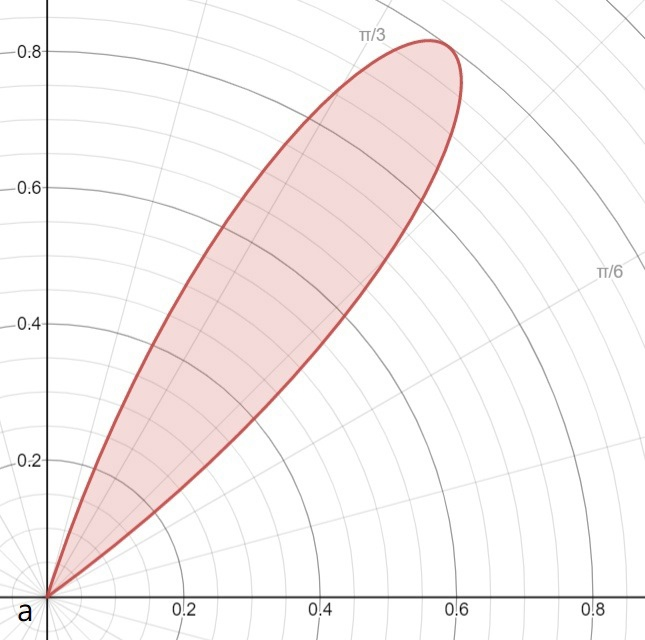
\includegraphics[scale=0.44]{Primer_1.jpg}
		\label{fig:universe}
		\caption{Пример того, как частную производную следует искать как предел по множеству в точке $a$.}
	\end{figure}
	\[\frac{\partial f}{\partial x}(a) = \lim\limits_{\substack{(x, y)\to (a_1, a_2)\\(x, y) \in X}} \frac{\partial f} {\partial x}(x, y)\]
	\[\frac{\partial f}{\partial y}(a) = \lim\limits_{\substack{(x, y)\to (a_1, a_2)\\(x, y) \in X}} \frac{\partial f} {\partial y}(x, y)\]
	
	\subsection{Дифференцируемость функции в точке}
	
	Некоторые замечания, которые нужны для определения дифференцируемости функции в точке:\\
	
	Рассмотрим $w = f(x)$, она определена в $\mathscr{U}(a), a = (a_1, \ldots,a_m), \Delta x = (\Delta x_1, \ldots, \Delta x_m): a + \Delta x = (a_1 + \Delta x_1, \ldots , a_m + \Delta x_m) \in \mathscr{U}(a)$\\
	
	Рассмотрим $\rho = \sqrt{(\Delta x_1)^2 + \ldots + (\Delta x_m)^2}$,  $\rho \to 0 \Leftrightarrow \Delta x \to \bar0$, где $\bar0 = \overbrace{(0, 0\ldots, 0)}^{m}$.\\
	
	$\Delta f(a, \Delta x) = f(a + \Delta x) - f(a)$ -- Полное приращение функции в точке а, соответствующее приращению аргументов $\Delta x = (\Delta x_1, \ldots, \Delta x_m)$.\\
	
	\underline{\textbf{Определение:}} Функция $f$ называется дифференцируемой в точке а, если 
	
	\textbf{Условие 1:}
	\[\Delta f(a, \Delta x) = A_1 \Delta x_1 + \ldots + A_m \Delta x_m + \alpha_1(\Delta x) \Delta x_1 + \ldots + \alpha_m (\Delta x)\Delta x_m\] 
	где $A_j$ -- постоянные, $j = 1,\ldots,m$, не зависят от $\Delta x$, $\alpha_j = \alpha_j(\Delta x)$ -- б.м. функции при $\Delta x \to 0$; $\alpha_j = 0$ при $\bar{\Delta x} = \bar0$.\\
	
	\textbf{Условие 2:}
	\[\Delta f(a, \Delta x) = A_1 \Delta x_1 + \ldots + A_m \Delta x_m + o(\rho), \rho\to 0\]  
	\begin{center}
		(По сути $\rho$ -- расстояние от точки $\Delta x$ до $\bar0$).
	\end{center}
	
	\textbf{Предложение.} Условия 1 и 2 определения дифференцируемости функции в точке эквиваленты.\\
	
	\textbf{Доказательство.}
	
	1 $\Rightarrow$ 2
	
	Покажем, что $\alpha_1(\Delta x)\Delta x_1 + \ldots + \alpha_m(\Delta x)\Delta x_m = o(\rho), \; \rho \rightarrow 0, \; \rho \not= 0$.
	
	Заметим, что \[\left|\frac{\Delta x_j}{\rho}\right| \leq 1, \; \rho = \sqrt{(\Delta x_1)^2 + \ldots + (\Delta x_m)^2}\]
	\[|\alpha_1\Delta x_1 + \ldots \alpha_m\Delta x_m| \leq \rho \cdot (|\alpha_1|\frac{|\Delta x_1|}{\rho} + \ldots + |\alpha_m|\frac{|\Delta x_m|}{\rho}) \leq \rho \cdot (|\alpha_1| + \ldots + |\alpha_m|)\]
	
	В силу того, что $\rho \to 0 \Leftrightarrow \Delta x \to \bar0$, $|\alpha_1| + \ldots + |\alpha_m|$ также стремиться к нулю, как конечная сумма б.м. функций.\\
	Значит, $\rho \cdot (|\alpha_1| + \ldots + |\alpha_m|) = o(\rho)$. Показали, что это выражение действительно есть б.м. функция.\\
	
	2 $\Rightarrow$ 1 
	
	\[o(\rho) = \frac{\rho^2}{\rho} \frac{o(\rho)}{\rho} = \frac{(\Delta x_1)^2 + \ldots + (\Delta x_m)^2}{\rho} \frac{o(\rho)}{\rho}\]
	\[o(\rho) = (\frac{\Delta x_1}{\rho}\frac{o(\rho)}{\rho})\Delta x_1 + \ldots + (\frac{\Delta x_m}{\rho}\frac{o(\rho)}{\rho})\Delta x_m \]
	
	Понятно, что $\alpha_j = \frac{\Delta x_j}{\rho}\frac{o(\rho)}{\rho}$, но $\frac {\Delta x_j}{\rho}$ величина ограниченная, а $\frac {o(\rho)}{\rho} \to 0, \; \rho \to 0 \Rightarrow $ при $\Delta x \to \bar 0$.
	$\alpha_j = 0, \; j = 1, \ldots, m$, только при $\Delta x = \bar0$.
	
	\textit{Доказано.}
	
	
	\subsection{Достаточные условия дифференцируемости функции в точке}
	
	\underline{\textbf{Теорема 2.}} Пусть $w = f(x)$ определена в $\mathscr{U}(a) \subset \mathds{E}^m$
	и в этой окрестности существуют $\frac{\partial f}{\partial x_j}, \; j = 1, \ldots, m$. 
	Если  $\frac{\partial f}{\partial x_j}, \; j = 1, \ldots, m$ непрерывны в точке $a$, то функция $f$ дифференцируема в точке $a$.\\
	
	\textbf{Докательство.} Проведем доказательство для $m = 2, \; w = f(x, y), \; a = (a_1, a_2)$.
	
	Рассмотрим точку $(a_1 + \Delta x, a_2 + \Delta y) \in \mathscr{U}(a)$.\\
	
	Рассмотрим 
	\[\Delta f(a, (\Delta x, \Delta y)) = f(a_1 + \Delta x, a_2 + \Delta y) - f(a_1, a_2)\]
	\begin{multline*}
		\Delta f(a, (\Delta x, \Delta y)) = f(a_1 + \Delta x, a_2 + \Delta y)
		- f(a_1, a_2 + \Delta y) + f(a_1, a_2 + \Delta y) - f(a_1, a_2)
	\end{multline*}
	
	Введем функцию $\varphi(x) = f(x, a_2 + \Delta y)$ и $\psi(y) = f(a_1, y)$
	\begin{multline*}
		\Delta f(a, (\Delta x, \Delta y)) = \Delta\varphi(a_1, \Delta x) + \Delta\psi(a_2, \Delta y) = \\
		= \varphi(a_1 + \Delta x) - \varphi(a_1) + \psi(a_2 + \Delta y) - \psi(a_2)
	\end{multline*}
	
	По теореме Лагранжа для функции одной переменной: $\exists \theta_1: ~0 < \theta_1 < 1$ и $\exists \theta_2: ~ 0 < \theta_2 < 1:$
	\[f(a_1 + \Delta x, a_2 + \Delta y) - f(a_1, a_2 + \Delta y) = f'_x(a_1 + \theta_1 \Delta x, a_2 + \Delta y)\Delta x\]
	\[f(a_1, a_2 + \Delta y) - f(a_1, a_2) = f'_y(a_1, a_2 + \theta_2 \Delta y)\Delta y\]
	\[f'_x(a_1 + \theta_1\Delta x, a_2 + \Delta y) = f'_x(a_1, a_2) + \alpha_1(\Delta x, \Delta y); \; \alpha_1 \to 0, \; (\Delta x, \Delta y) \to (0, 0)\]
	\[f'_y(a_1, a_2 + \theta_2 \Delta y) = f'_y(a_1, a_2) + \alpha_2(\Delta x, \Delta y); \; \alpha_2 \to 0, \; (\Delta x, \Delta y) \to (0, 0)\]
	\[\Delta f(a, (\Delta x, \Delta y)) = f'_x(a)\Delta x +f'_y(a)\Delta y + \alpha_1\Delta x + \alpha_2 \Delta y\]
	
	Получили в точности определение дифференцируемости функции $f$ в точке $a$.
	
	\textit{Доказано.}\\
	
	\textbf{Примеры.} (Доказательство дифференцируемости ф-ции в точке)\\
	$w = f(x, y), \; \bar0 = (0,0), \; \rho = \sqrt{x^2 + y^2 }$\\ 
	$f(x, y) - f(0, 0)= \frac{\partial f}{\partial x}(0, 0)\Delta x + \frac{\partial f}{\partial y}(0, 0)\Delta y + o(\rho), \; \rho \to 0$.\\
	
	\textbf{Пример 1.} $f(x, y) = y^2 \sin x$\\
	
	Заметим, что $f(x, 0) = f(0, y) = f(0, 0) = 0$\\
	
	Из определения частной производной: $\frac{\partial f}{\partial x}(0,0) = \lim\limits_{x\to0} \frac {f(x, 0) - f(0, 0)} {x} = 0$.\\
	$\frac{\partial f}{\partial y}(0,0) = \lim\limits_{y\to0} \frac {f(0, y) - f(0, 0)} {y} = 0$.\\
	
	Частные производные равны нулю, значит, надо показать, что $f(x, y) = o(\rho), \; \rho \to 0$.
	Надо показать, что $F(x, y) = \frac{f(x, y)}{\sqrt{x^2 + y^2}} \to 0$, при $(x, y) \to (0, 0)$.\\
	$|F(x, y)| = |\frac{y^2 \sin x}{\sqrt{x^2 + y^2}}| \leq \frac{y^2}{\sqrt{x^2 + y^2}} \leq [\;\; |y| \leq \sqrt{x^2 + y^2}\;\;] \leq \frac{\sqrt{x^2 + y^2}^2}{\sqrt{x^2 + y^2}} = \sqrt{x^2 + y^2} \leq \delta = \varepsilon$\\
	$[\forall\varepsilon > 0  ~\exists\delta = \delta(\varepsilon) = \varepsilon: \forall(x, y): 0 < \rho = \sqrt{x^2 + y^2} < \delta \mapsto |F(x, y)| < \varepsilon] \stackrel{def}{=} [\lim\limits_{(x, y) \to (0, 0)} F(x, y) = 0] \Leftrightarrow [f(x, y) = o(\rho), \rho \to 0]$.\\
	
	\textbf{Пример 2.} $f(x, y) = \sqrt{|xy|}, \; \bar0 = (0, 0)$\\
	$f(x, 0) = f(0, y) = f(0, 0) = 0 \Rightarrow \frac{\partial f}{\partial x}(0, 0) = \frac{\partial f}{\partial y}(0, 0) = 0$\\
	$F(x, y) = \frac{\sqrt{|xy|}}{\sqrt{x^2 + y^2}}$.
	
	Перейдем к полярным координатам: $x = \rho \cos \varphi, \; y = \rho \sin \varphi$, $F(x, y) = \sqrt{|\cos \varphi\sin \varphi|}$\\
	$\varphi = \frac{\pi}{2} \Rightarrow F(\rho, \varphi) = 0$\\
	$\varphi = \frac{\pi}{4} \Rightarrow F(\rho, \varphi) = \frac{1}{\sqrt{2}} \not= 0$\\
	Значит, $f$ не является дифференцируемой в точке (0, 0).\\
	
	\textbf{Пример 3.(Очень важный для понимания теории)} 
	\begin{equation*}
		f(x, y) = 
		\begin{cases}
			(x^2 + y^2)\sin{\frac{1}{\sqrt{x^2 + y^2}}}, & x^2 + y^2 \not=0,\\
			0, & x^2 + y^2 = 0
		\end{cases}
	\end{equation*}
	
	$f(x, 0) = x^2\sin{\frac{1}{|x|}}, x \not =0$
	
	$f(0, y) = y^2\sin{\frac{1}{|y|}}, y \not =0$
	
	$f(0,0) = 0$
	
	$\frac{\partial f}{\partial x}(0, 0) = \lim\limits_{x \to 0} = \frac{f(x, 0) - f(0, 0))}{x} = \lim\limits_{x \to 0} x\sin{\frac{1}{|x|}} = 0$ 
	
	$\frac{\partial f}{\partial y}(0, 0) = \lim\limits_{y \to 0} = \frac{f(0, y) - f(0, 0))}{y} = \lim\limits_{y \to 0} y\sin{\frac{1}{|y|}} = 0$\\
	
	Теперь докажем, что эта функция дифференцируема в (0, 0)
	
	Введем функцию \[F(x, y) = \frac{f(x, y)}{\sqrt{x^2 + y^2}} = \sqrt{x^2 + y^2}\sin{\frac{1}{\sqrt{x^2 + y^2}}}\]
	
	\[|F(x, y)| \leq \sqrt{x^2 + y^2} < \delta = \varepsilon\]
	
	\[\forall\varepsilon > 0  ~\exists\delta = \delta(\varepsilon) = \varepsilon: \forall(x, y): 0 < \rho = \sqrt{x^2 + y^2} < \delta \mapsto |F(x, y)| < \varepsilon] \stackrel{def}{=}\]
	
	\[ [ \lim\limits_{(x, y) \to (0, 0)} F(x, y) = 0] \Leftrightarrow [f(x, y) = o(\rho), \rho \to 0] \Rightarrow\]
	
	\[\Rightarrow f \text{дифференцируема в (0, 0)}\]
	
	Посмотрим на частные производные этой функции по x и y вне точки (0, 0):\\
	
	\[\frac{\partial f}{\partial x}(x, y) = 2x\sin{\frac{1}{\sqrt{x^2+y^2}}} -\frac{x^2+y^2}{(\sqrt{x^2+y^2})^3} \cos{\frac{1}{\sqrt{x^2+y^2}}}\]
	
	$\lim\limits_{(x, y) \to (0, 0)} \frac{\partial f}{\partial x}(x, y)$ не существует $\Rightarrow f'_x$ не является непрерывной в (0, 0).\\
	Пример показывает, что непрерывность частных производных в точке не является необходимым условием дифференцируемости функции.\\
	
	\textbf{Замечание.} Непрерывность частных производных функции $f$ в точке не является необходимым условием дифференцируемости функции в точке. Это условие достаточно (Теорема 2).\\
	
	\subsection{Дифференцируемость сложной функции}
	
	Рассматриваем функции $x_j = \varphi_j(t)$ в окрестности точки $t^0 = (t_1^0, \ldots, t_k^0)\in \mathds{E}^k, \; j = 1, \ldots, m$. Рассматриваем функцию $w = f(x),$ которая определена в окрестности точки $a = (a_1, \ldots, a_m)$, причем $a_j = \varphi_j(t^0), \; j = 1, \ldots, m$. $F(t) = f(\varphi_1(t), \ldots, \varphi_m(t))$ -- суперпозиция функций $f$ и функций $\varphi_1(t) \ldots$ (сложная функция)\\
	
	\underline{\textbf{Теорема 3 [О дифференцируемости сложной функции]:}}
	
	Пусть функции $\varphi_j, \; j = 1, \ldots, m$ дифференцируемы в точке $t^0$, функция $f$ дифференцируема в точке $а$, причем $a_j = \varphi_j(t^0), \; j = 1, \ldots,m$. Тогда $F(t) = f(\varphi_1(t), \ldots, \varphi_m(t))$ дифференцируема в точке $t^0$ и 
	\[\frac{\partial F}{\partial t_j}(t^0) = \frac{\partial f}{\partial x_1}(a) \frac{\partial \varphi_1}{\partial t_j}(t^0	) + \frac{\partial f}{\partial x_2}(a) \frac{\partial \varphi_2}{\partial t_j}(t^0	) + \ldots + \frac{\partial f}{\partial x_m}(a) \frac{\partial \varphi_m}{\partial t_j}(t^0), j = 1, \ldots, k\].
	
	\textbf{Доказательство.} $t^0 + \Delta t \in \mathscr{U}(t^0), a + \Delta x \in \mathscr{U}(a), \rho = \sqrt{(\Delta t_1)^2 + \ldots + (\Delta t_k)^2}$.\\
	
	Условия дифференцируемости функции $\varphi_j$ в точке $t^0$:
	
	\[\Delta \varphi_j(t^0, \Delta t) = \frac{\partial \varphi_j}{\partial t_1}(t^0)\Delta t_1 + \ldots + \frac{\partial \varphi_j}{\partial t_k}(t^0)\Delta t_k + o(\rho), \; \rho \to 0; \; \rho \to 0 \Leftrightarrow \Delta t \to \bar0.\]
	
	Условия дифференцируемости функции $f$ в точке a:
	\[\Delta f(a, \Delta x) = \frac {\partial f}{\partial x_1}(a)\Delta x_1 + \ldots + \frac {\partial f}{\partial x_m}(a)\Delta x_m + \alpha_1 \Delta x_1 + \ldots + \alpha_m \Delta x_m.\]
	
	Подставим вместо $\Delta x_1 \ldots \Delta x_m$ приращения функции $\varphi$:\\
	\begin{multline*}
		\Delta f(a, \Delta x) = \frac {\partial f}{\partial x_1}(a)\left[\frac{\partial \varphi_1}{\partial t_1}(t^0)\Delta t_1 + \ldots + \frac{\partial \varphi_1}{\partial t_k}(t^0)\Delta t_k + o(\rho)\right] + \ldots\\
		\ldots + \frac {\partial f}{\partial x_m}(a) \left[\frac{\partial \varphi_m}{\partial t_1}(t^0)\Delta t_1 + \ldots + \frac{\partial \varphi_m}{\partial t_k}(t^0)\Delta t_k + o(\rho)\right] +\\ +\alpha_1\left[\frac{\partial \varphi_1}{\partial t_1}(t^0)\Delta t_1 + \ldots + \frac{\partial \varphi_1}{\partial t_k}(t^0)\Delta t_k + o(\rho)\right] + \ldots \\
		\ldots + \alpha_m \left[\frac{\partial \varphi_m}{\partial t_1}(t^0)\Delta t_1 + \ldots + \frac{\partial \varphi_m}{\partial t_k}(t^0)\Delta t_k + o(\rho)\right].
	\end{multline*}
	
	Перегруппируем слагаемые:
	\begin{multline*}
		\left[\frac{\partial f}{\partial x_1}(a)\frac{\partial\varphi_1}{\partial t_1}(t_0) + \ldots + \frac{\partial f}{\partial x_m}(a)\frac{\varphi_m}{\partial t_1}(t_0)\right]\Delta t_1 + \ldots\\
		\ldots + \left[\frac{\partial f}{\partial x_1}(a)\frac{\partial\varphi_1}{\partial t_k}(t_0) + \ldots + \frac{\partial f}{\partial x_m}(a)\frac{\varphi_m}{\partial t_k}(t_0)\right]\Delta t_k + \\
		+o(\rho)\left[\frac{\partial f}{\partial x_1}(a) + \ldots + \frac{\partial f}{\partial x_m}(a) + \alpha_1 + \ldots + \alpha_m\right] + \\
		+\rho\left[\alpha_1\frac{\partial \varphi_1}{\partial t_1}(t^0) + \ldots + \alpha_m \frac{\partial \varphi_m}{\partial t_1}(t^0)\right]\frac{\Delta t_1}{\rho} + \ldots \\
		\ldots + \rho\left[\alpha_1\frac{\partial \varphi_1}{\partial t_k}(t^0) + \ldots + \alpha_m \frac{\partial \varphi_m}{\partial t_k}(t^0)\right]\frac{\Delta t_k}{\rho}. 
	\end{multline*}
	
	\[ \Delta F(t^0, \Delta t) = \frac{\partial F}{\partial t_1}(t^0)\Delta t_1 + \ldots + \frac{\partial F}{\partial t_k}(t^0)\Delta t_k + o(\rho)\gamma + \rho\Lambda_1 + \ldots + \rho \Lambda_k\]
	
	$\gamma$ - ограниченна, $\Delta x_j = \Delta \varphi_j \xrightarrow[\Delta t \to \bar 0 ]{} 0,\;
	\rho \to 0 \Leftrightarrow \Delta t \to \bar0 = (0, \ldots, 0). \; \Rightarrow \alpha_j \to 0$, при $\rho \to 0$
	
	\[\Lambda_j = [\alpha_1\frac{\partial \varphi_1}{\partial t_1}(t^0) + \ldots + \alpha_m \frac{\partial \varphi_m}{\partial t_1}(t^0)]\frac{\Delta t_j}{\rho} \to 0, \; \rho \to 0\]
	
	Перепишем:
	\[\Delta F(t^0, \Delta t) = \frac{\partial F}{\partial t_1}(t^0)\Delta t_1 + \ldots + \frac{\partial F}{\partial t_k}(t^0)\Delta t_k + o(\rho), \; \rho \to 0\]
	
	\textit{Доказано.}
	
	\subsection{Дифференциал. Инвариантность формы дифференциала отностительно замены переменных.}
	
	Рассматриваем функцию $w = f(x)$ определенную в $\mathscr{U}(a) \subset \mathds{E}^m$. Мы предполагаем, что $f$ дифференцируема в точке а. Поскольку функция дифференцируема в точке а, то \[\Delta f(a, \Delta x) = \frac{\partial f}{\partial x_1}(a)\Delta x_1 + \ldots + \frac{\partial f}{\partial x_m}(a) \Delta x_m + o(\rho), \rho \to 0\]
	
	\underline{\textbf{Определение:}} Дифференциалом функции $f$ в точке а называется главная линейная часть (относительно $\Delta x_j$) приращения функции $f$ в точке а, соответствующая приращению аргументов $\Delta x = (\Delta x_1, \ldots, \Delta x_n)$.
	\[df(a) = \frac{\partial f}{\partial x_1}(a)\Delta x_1 + \ldots + \frac{\partial f}{\partial x_m}(a)\Delta x_m\]
	Поскольку дифференциал независимой переменной $x_j$ есть произвольное число, то $dx_j = \Delta x_j$.
	\[df(a) = \frac{\partial f}{\partial x_1}(a)dx_1 + \ldots + \frac{\partial f}{\partial x_m}(a)dx_m ~~~~~~~(*)\]
	
	\textbf{Предложение.[Инвариантность формы 1-го дифференциала]} 
	
	Выражение (*) универсально, оно справедливо и в случае, когда $x_j = \varphi_j(t), \; t \in \mathscr{U}(t^0) \subset \mathds{E}^k, \; a_j = \varphi_j(t^0), \; j = 1, \ldots, \; m$ ($\varphi_j$ дифференцируема в точке $t^0$).
	
	\textit{Доказательство.}
	\[d\varphi_j(t^0) = \frac {\partial \varphi_j}{\partial t_1}(t^0)dt_1 + \ldots + \frac {\partial \varphi_j}{\partial t_k}(t^0)dt_k, \; j = 1, \ldots, m\]
	
	Введем функцию $F(t) = f(\varphi_1(t), \ldots, \varphi_m(t))$
	\[dF(t^0) = \frac{\partial F}{\partial t_1}(t^0)dt_1 + \ldots +\frac{\partial F}{\partial t_k}(t^0)dt_k \]
	\[dF(t^0) = \left[\frac{\partial f}{\partial x_1}(a) \frac{\partial \varphi_1}{\partial t_1}(t^0) + \ldots + \frac{\partial f}{\partial x_m}(a) \frac{\partial \varphi_m}{\partial t_1}(t^0) \right]dt_1 + \ldots\]
	\[+ \left[\frac{\partial f}{\partial x_1}(a) \frac{\partial \varphi_1}{\partial t_k}(t^0) + \ldots + \frac{\partial f}{\partial x_m}(a) \frac{\partial \varphi_m}{\partial t_k}(t^0) \right] dt_k\]
	
	Перегруппируем:
	\[dF(t^0) = \frac{\partial f}{\partial x_1}(a) \left[\frac{\partial \varphi_1}{\partial t_1}(t^0) dt_1 + \ldots + \frac{\partial \varphi_1}{\partial t_k}(t^0) dt_k \right] + \ldots\] \[+\frac{\partial f}{\partial x_m}(a) \left[ \frac{\partial \varphi_m}{\partial t_1}(t^0) dt_1 + \ldots + \frac{\partial \varphi_m}{\partial t_k}(t^0) dt_k \right]\]
	
	Получаем:
	\[dF(t^0) = \frac{\partial f}{\partial x_1}(a)dx_1 + \ldots + \frac{\partial f}{\partial x_m}(a)dx_m\]
	\textit{Доказано.}
	
	\subsection{Производная по направлению и градиент, их связь и  геомертический смысл.}
	Рассматриваем функцию $w = f(x)$ определенную в $\mathscr{U}(a) \subset \mathds{E}^m$. Мы предполагаем, что $f$ дифференцируема в точке а. Возьмём единичный вектор $\vec{n} = (\cos \alpha_1, \ldots, \cos \alpha_m), |\vec{n}| = 1$.
	
	\begin{equation*}
		l: 
		\begin{cases}
			x_1 = a_1 + t\cos \alpha_1;\\
			\ldots\\
			\ldots\\
			\ldots\\
			x_m = a_m + t\cos \alpha_m;
		\end{cases}
	\end{equation*}
	
	Рассмотрим суперпозицию:
	\[F(t) = f(a_1 + t\cos\alpha_1, \ldots, a_m + t\cos\alpha_m)\]
	$F$ дифференцируема в точке $t = 0$.\\
	
	\underline{\textbf{Определение:}} Производной функции $f$ по направлению $l$ в точке $x = a$ называется производная функции $F$ в точке $t = 0$.\\
	
	\underline{\textbf{Обозначения.}}
	\[\frac{\partial f}{\partial l}(a) = \lim\limits_{t \to 0} \frac{f(a_1 + t\cos\alpha_1, \ldots, a_m + t\cos\alpha_m) - f(a)}{t}\]
	
	\[\frac{\partial f}{\partial l}(a) = \frac{\partial f}{\partial x_1}(a)\cos\alpha_1 + \ldots + \frac{\partial f}{\partial x_m}(a)\cos\alpha_m\]\\
	
	\underline{\textbf{Определение:}} Градиентом функции $f$ называется вектор \[\mathrm{grad}{f(a)} = (\frac{\partial f}{\partial x_1}(a), \ldots, \frac{\partial f}{\partial x_m}(a))\]
	
	Из этого определения и выражения для производной по направлению $l$ в точке $a$ функции $f$ мы получаем:
	\[\frac{\partial f}{\partial l}(a) = (\mathrm{grad}{f(a), \vec{n}})\]
	
	\underline{\textbf{Предложение.}}
	Градиент функции $f$ в точке $a$ характеризует направление и величину максимального роста производной по направлению функции $f$ в точке $a$.
	
	\textit{Доказательство.}
	
	По определению производной по направлению в точке $a$:
	\[\frac{\partial f}{\partial l}(a) = |\mathrm{grad}{f(a)}| |\vec{n}|\cos\varphi = |\mathrm{grad}{f(a)}|\cos\varphi\]
	
	$\cos\varphi$ имеет наибольшее значение равное 1 $\Rightarrow$
	$cos\varphi = 1 \Rightarrow \vec{n}$ и $\mathrm{grad}$ -- направление совпадают, т.к. в этом случае $\varphi = 0$.
	
	\textit{Доказано.}
	\subsection{Необходимые условия дифференцируемости}
	
	\textbf{Необходимое условие 1.}
	
	$[f$ дифференцируема в точке а$] \Rightarrow [\exists \frac{\partial f}{\partial x_j}(a), \; j = 1, \ldots, m]$\\
	
	\textbf{Доказательство.}
	
	Возьмем $j = k$, рассматриваем $\Delta x = (0, \ldots, 0, \Delta x_k, 0, \ldots, 0)$. Тогда $\Delta f(a, \Delta x) = \Delta_k f(a, \Delta x_k)$. Тогда используя $1$-ое условие определения получим:
	
	\[\Delta f(a, \Delta x) = A_1 \Delta x_1 + \ldots + A_m \Delta x_m + \alpha_1(\Delta x) \Delta x_1 + \ldots + \alpha_m (\Delta x)\Delta x_m\] 
	
	Получаем следующее: 
	\[\Delta_k f(a, \Delta x_k) = A_k\Delta x_k + \alpha_k\Delta x_k\]
	\[\frac{\Delta_k f(a, \Delta x_k)}{\Delta x_k} = A_k + \alpha_k \to A_k, \; \Delta x_k \to 0 \Rightarrow A_k = \frac{\partial f}{\partial x_k} (a)\]
	
	В силу произвольности мы доказано для всех переменных.
	
	\textit{Доказано.}\\
	
	Таким образом мы уточнили определение, например, перепишем определение $1$:
	\[\Delta f(a, \Delta x) = \frac{\partial f}{\partial x_1}(a) \Delta x_1 + \ldots + \frac{\partial f}{\partial x_m}(a) \Delta x_m + \alpha_1(\Delta x) \Delta x_1 + \ldots + \alpha_m (\Delta x)\Delta x_m\]
	
	\textbf{Необходимое условие 2.} Если $w = f(x), x \in \mathds{E}^m$ дифференцируема в точке а, то $f$ непрерывна в точке $a$.\\
	
	\textbf{Доказательство.}\\
	$\Delta f(a, \Delta x) = f(a + \Delta x) - f(a) = \frac{\partial f}{\partial x_1}(a) \Delta x_1 + \ldots + \frac{\partial f}{\partial x_m}(a) \Delta x_m + \alpha_1(\Delta x) \Delta x_1 + \ldots + \alpha_m (\Delta x)\Delta x_m$.\\
	Если $\Delta x \to \bar0$, то $f(a + \Delta x) - f(a) \to 0 \Rightarrow $ f непрерывна в точке а.
	
	\textit{Доказано.}\\
	
	\textbf{Необходимое условие 3.}(Не было в лекции Знаменской)\\
	Пусть функция $f$ 	дифференцируема в  точке $(x_0, y_0, z_0)$. Тогда в этой точке функция $f$ имеет производную по любому направлению и эта производная находится по формуле 
	\[\frac{\partial f}{\partial l}(x_0, y_0, z_0) = \frac{\partial f}{\partial x}\cos \alpha + \frac{\partial f}{\partial y}\cos\beta + \frac{\partial f}{\partial z}\cos \gamma\]
	\begin{center}
		[Взято из Кудрявцева, Том 2, стр. 267]
	\end{center}
	
	%=======================================================================================
	
	%БИЛЕТ 4
	%=======================================================================================
	\newpage
	\section{Билет 4}
	
	\subsection{Частные производные высших порядков.}
	
	\underline{\textbf{Определение:}} Пусть $\omega = f(x)$ - дифференцируема в $D \subset \mathbb{E}^m$, $D$ - область.
	И $\forall x \in D \text{ }\exists \frac{\partial{f}}{\partial{x_j}}(x), \; j = \overline{1, m}$.
	
	Пусть $g_j = \frac{\partial{f}}{\partial{x_j}}$, и в точке $x$:  $\exists\frac{\partial{g_j}}{\partial{x_k}}(x)$. Тогда
	\[
	\frac{\partial{g_j}}{\partial{x_k}}(x) = \frac{\partial{ }}{\partial{x_k}}\left(\frac{\partial{f}}{\partial{x_j}}\right)(x)
	\]
	называется частной производной 2-го порядка функции $f$ в точке $x$. Частные производные высших порядков определяются так же.\\
	
	\textbf{Обозначения:} 
	\[		
	\frac{\partial^2f}{\partial{x_k}\partial{x_j}}(x), \text{   } f^{''}_{x_jx_k}(x), \text{   } f^{(2)}_{x_jx_k}(x)
	\]
	\[
	j = k: \text{ }\frac{\partial^2f}{\partial{x_j}^2}(x)
	\]
	
	\textbf{Примечание:} если $k\neq j$, производная $\frac{\partial^2f}{\partial x_k\partial x_j}$ называется смешанной.
	
	\subsection{Независимость смешанной частной производной от порядка дифференцирования.}
	
	\textbf{Примеры:}
	
	\begin{enumerate}
		
		\item 
		\begin{align*}
			f(x, y) &= \text{arctg}\left(\frac{x}{y}\right)\\
			\frac{\partial{f}}{\partial{x}} &= \frac{1}{1+\frac{x^2}{y^2}}\cdot\frac{1}{y} = \frac{y}{y^2+x^2}\\
			\frac{\partial{f}}{\partial{y}} &= \frac{1}{1+\frac{x^2}{y^2}}\cdot\left(-\frac{x}{y^2}\right) = -\frac{x}{y^2+x^2}\\
			\frac{\partial^2f}{\partial{y}\partial{x}} &= \frac{y^2+x^2-2y^2}{(x^2+y^2)^2} = \frac{x^2-y^2}{(x^2+y^2)^2}\\
			\frac{\partial^2f}{\partial{x}\partial{y}} &= -\frac{y^2+x^2-2x^2}{(x^2+y^2)^2} = \frac{x^2-y^2}{(x^2+y^2)^2}
		\end{align*}
		\[
		\frac{\partial^2f}{\partial{x}\partial{y}} = \frac{\partial^2f}{\partial{y}\partial{x}}
		\]
		
		\item 
		\vspace{10mm}
		$$ f(x, y) = 
		\begin{cases*} 
			xy\cdot\frac{x^2-y^2}{x^2+y^2},& \text{$x^2+y^2\neq 0$}\\
			0,& \text{$x^2+y^2= 0$}
		\end{cases*}$$
		\begin{align*}
			f(x, 0) &= f(0, y) = f(0, 0) = 0 \Rightarrow \frac{\partial f}{\partial x}(0, 0) = \frac{\partial f}{\partial y}(0, 0) = 0\\&\\
			f^{'}_{x} &= y\frac{x^2-y^2}{x^2+y^2}+xy\frac{2x(x^2+y^2) - 2x(x^2-y^2)}{(x^2+y^2)^2} = \frac{y(x^4-y^4)+4x^2y^3}{(x^2+y^2)^2}\\
			f^{'}_{y} &= x\frac{x^2-y^2}{x^2+y^2}+xy\frac{-2y(x^2+y^2) - 2y(x^2-y^2)}{(x^2+y^2)^2} = \frac{x(x^4-y^4)+4x^3y^2}{(x^2+y^2)^2}\\&\\
			\frac{\partial f}{\partial x}&(x, y) =
			\begin{cases*}
				\frac{yx^4-y^5+4x^2y^3}{(x^2+y^2)^2}, &\text{$x^2+y^2\neq 0$}\\
				0, &\text{$x^2+y^2=0$}
			\end{cases*}\\
			\frac{\partial f}{\partial y}&(x, y) =
			\begin{cases*}
				\frac{x^5-xy^4-4x^3y^2}{(x^2+y^2)^2}, &\text{$x^2+y^2\neq 0$}\\
				0, &\text{$x^2+y^2=0$}
			\end{cases*}\\&\\
			\frac{\partial^2f}{\partial y\partial x}&(0, 0) = \lim\limits_{y\to 0}\frac{f^{'}_x(0, y) - f^{'}_x(0, 0)}{y} = \lim\limits_{y\to 0}\frac{-y^5}{y^5} = -1\\
			\frac{\partial^2f}{\partial x\partial y}&(0, 0) = \lim\limits_{x\to 0}\frac{f^{'}_y(x, 0) - f^{'}_y(0, 0)}{x} = \lim\limits_{x\to 0}\frac{x^5}{x^5} = 1
		\end{align*}
		\[
		\frac{\partial^2f}{\partial{x}\partial{y}} \neq \frac{\partial^2f}{\partial{y}\partial{x}}
		\]
		\vspace{5mm}
		
	\end{enumerate}
	
	Из этих примеров видно, что в общем случае смешанные производные зависят от порядка дифференцирования.
	\vspace{5mm} 
	
	\underline{\textbf{Теорема:}} Пусть в $\mathscr{U}(a) \subset \mathbb{E}^2$ определены $\frac{\partial^2f}{\partial x\partial y}$ и $\frac{\partial^2f}{\partial y\partial x}$, и эти производные непрерывны в точке $a = (a_1, a_2)$, тогда
	\[
	\frac{\partial^2f}{\partial{x}\partial{y}}(a) = \frac{\partial^2f}{\partial{y}\partial{x}}(a)
	\]
	
	\textbf{Доказательство:} Рассмотрим функцию
	\[
	U(x, y) = f(x, y) - f(x, a_2) - f(a_1, y) + f(a_1, a_2)
	\]
	
	Пусть $\Pi = \{(x, y) : |x - a_1|\leqslant r_1, |y-a_2| \leqslant r_2\}$, $\Pi \subset \mathscr{U}(a)$, где определены смешанные производные. Фиксируем $y\in (a_2-r_2, a_2+r_2)$ и на интервале $(a_1-r_1, a_1+r_1)$ рассмотрим функцию 
	\[
	\varphi(x) = f(x, y) - f(x, a_2)
	\]
	$\varphi$ дифференцируема на интервале $(a_1-r_1, a_1+r_1)$ и $U(x, y) = \varphi(x) - \varphi(a_1)$.
	Тогда, по теореме Лагранжа $\exists \theta_1: 0<\theta_1<1$:
	\[
	U(x, y) = \varphi^{'}(a_1 + \theta_1\Delta x)\Delta x
	\]
	где $\Delta x = x-a_1$
	\[
	U(x, y) = [f^{'}_x(a_1+\theta_1\Delta x, y)-f^{'}_x(a_1+\theta_1\Delta x, a_2) ]\Delta x
	\]
	
	К выражению, стоящему в [...] применим теорему Лагранжа.
	
	$\exists\theta_2: 0<\theta_2<1$:
	\[
	U(x, y) = f^{''}_{xy}(a_1+\theta_1\Delta x, a_2+\theta_2\Delta y)\Delta y\Delta x
	\]
	где $\Delta y = y-a_2$.
	\vspace{5mm}
	
	Аналогично фиксируем $x\in(a_1-r_1, a_1+r_1)$ и на интервале $(a_2-r_2, a_2+r_2)$ получаем
	\[
	U(x, y) = f^{''}_{yx}(a_1+\theta_3\Delta x, a_2+\theta_4\Delta y)\Delta y\Delta x
	\]
	
	\[
	f^{''}_{yx}(a_1+\theta_3\Delta x, a_2+\theta_4\Delta y) = f^{''}_{xy}(a_1+\theta_1\Delta x, a_2+\theta_2\Delta y)
	\]
	Учитывая непрерывность в точке $a$ при $\Delta x\to0, \Delta y\to0$, получаем $f^{''}_{xy}(a) = f^{''}_{yx}(a)$.\\
	
	
	\underline{\textbf{Определение:}} Функция $\omega = f(x, y)$ называется $n$ раз дифференцируемой в точке $x = a\in \mathbb{E}^m$, если все ее частные производные порядка $n-1$ есть дифференцируемые функции
	\vspace{5mm}
	
	\underline{\textbf{Теорема:}} (без доказательства) Пусть $\omega = f(x, y)$ дважды дифференцируема в точке $a$, тогда
	\[
	\frac{\partial^2f}{\partial{x}\partial{y}}(a) = \frac{\partial^2f}{\partial{y}\partial{x}}(a)
	\]
	
	\subsection{Дифференциалы высших порядков. Отсутствие инвариантности их формы.}
	
	\underline{\textbf{Определение:}} Пусть $\omega = f(x)$ дважды дифференцируема в $D \subset \mathbb{E}^m$. $\forall x\in D $ $df(x) = \sum\limits_{j=1}^m\frac{\partial f}{\partial x_j}(x)dx_j$. Тогда дифференциалом 2 порядка будем называть
	\[
	d^2f(x) =d(df)(x) = \sum\limits_{j=1}^md\left(\frac{\partial f}{\partial x_j}\right)(x)dx_j= \sum\limits_{j=1}^m\left(\sum\limits_{k=1}^m
	\frac{\partial^2f}{\partial x_k\partial x_j}(x)dx_k\right)dx_j
	\]
	
	Дифференциалы высших порядков определяются таким же образом.
	\vspace{5mm}
	
	\textbf{Замечание:} Если рассмотреть дифференциал, как оператор
	\[
	d = \left(dx_1\frac{\partial}{\partial x_1}+\cdots+dx_m\frac{\partial}{\partial x_m}\right)
	\]
	
	То дифференциал $n$-ого порядка можно записать в виде
	\[
	d^n = \left(dx_1\frac{\partial}{\partial x_1}+\cdots+dx_m\frac{\partial}{\partial x_m}\right)^n
	\]
	
	\underline{\textbf{Предложение:}} Дифференциалы высших порядков не обладают свойством инвариантности формы.\\
	
	\textbf{Доказательство:} Пусть $\omega = f(x), $ $x_j=\varphi_j(t), $  $j=\overline{1, m}, $ $f, \varphi_j$ - дважды дифференцируемы.
	\[
	df(x) = \sum\limits_{j=1}^m\frac{\partial f}{\partial x_j}(x)dx_j, \text{ }dx_j = \sum\limits_{i=1}^k\frac{\partial \varphi_j}{\partial t_i}(i)dt_i
	\]
	
	\[
	d^2f(x) = \sum\limits_{i=1}^m\sum\limits_{j=1}^m
	\frac{\partial^2f}{\partial x_i\partial x_j}(x)dx_idx_j+\sum\limits_{j=1}^m\frac{\partial f}{\partial x_j}(x)d^2x_j
	\]
	причем
	\[
	\sum\limits_{j=1}^m\frac{\partial f}{\partial x_j}(x)d^2x_j \neq 0
	\]
	
	\subsection{Формула Тейлора для функций нескольких переменных.}
	
	\underline{\textbf{Теорема [Разложение с остаточным членом в форме Лагранжа]:}} Пусть функция $\omega = f(x)$ обладает непрерывными частными производными порядка $n+1$ в шаре $B_\delta(a)$, $\Delta x$ таково, что $a+\Delta x\in B_\delta(a)$. Тогда найдется $0<\theta<1$ такое, что 
	\[
	f(a+\Delta x) = f(a) + \sum\limits_{k=1}^n\frac{d^k f(a)}{k!}+r_{n+1}(\theta)
	\]
	где
	\[
	r_{n+1}(\theta) = \frac{d^{n+1}f(a+\theta \Delta x)}{(n+1)!}
	\]
	
	\textbf{Примечание:} $dx_j$ трактуется как $\Delta x_j$
	\vspace{5mm}
	
	\textbf{Доказательство:} $a+\Delta x\in B_\delta(a) \Rightarrow a-\Delta x\in B_\delta(a), $ $\forall t\in[-1, 1], a+t\Delta x\in B_\delta(a)$.
	
	\[
	f(a + t\Delta x) = f(a_1 + t\Delta x_1, \dots, a_m + t\Delta x_m) = \varphi(t)
	\]
	\[
	\varphi(0) = f(a)
	\]
	\[
	\varphi^{'}(t) = \sum\limits_{j=1}^m \frac{\partial f}{\partial x_j}(a+t\Delta x_j)\Delta x_j = df(a+t\Delta x)
	\]
	\[
	\varphi^{(k)}(t) = \sum\limits_{j_k=1}^m\cdots\sum\limits_{j_1=1}^m\frac{\partial^kf}{\partial x_{j_k}\dots\partial x_{j_1}}\Delta x_{j_1}\dots \Delta x_{j_k} = d^kf(a+t\Delta x)
	\]
	
	По формуле Тейлора
	\[
	\varphi(t) = \varphi(0) +\sum\limits_{k=1}^n\frac{\varphi^k(0)}{k!}t^k + r_{n+1}(\theta)
	\]
	где
	\[
	r_{n+1}(\theta) = \frac{\varphi^{(n+1)}(\theta t)}{(n+1)!}t^{(n+1)}
	\]
	
	Подставив $t=1$ получим требуемое равенство.
	\vspace{5mm}
	
	\underline{\textbf{Теорема [Разложение с остаточным членом в форме Пеано]:}}(без доказательства) Пусть $f$ n-раз дифференцируема в точке $x =a$, тогда
	\[
	f(a+\Delta x) = f(a) + \sum\limits_{k=1}^n\frac{d^kf(a)}{k!}+o(\rho),  \; \rho\to 0, \; \rho =  \rho(\Delta x, 0)
	\]
	
	%=======================================================================================
	
	%БИЛЕТ 5
	%=======================================================================================
	\newpage
	\section{Билет 5}
	
	\subsection{Необходимые определения и предложения билета.}
	
	\underline{\textbf{Определение:}} множество $Q = [a_1, b_1) \times [a_2, b_2) \times \dots \times [a_m, b_m)$ будем называть клеткой в $\mathbb{E}^m$.
	
	\vspace{3mm}
	
	\underline{\textbf{Определение:}} множество $G \subset \mathbb{E}^m$ будем называть клеточным, если оно является объединением \textbf{конечного} числа попарно непересекающихся клеток:
	\begin{equation*}
		G = \bigcup_{j = 1}^k Q_j, \hspace{10mm} Q_i \cap Q_j = \varnothing, \text{ }i \neq j.
	\end{equation*}
	
	
	\begin{figure}[h!]
		\begin{minipage}[h]{0.5\linewidth}
			\center{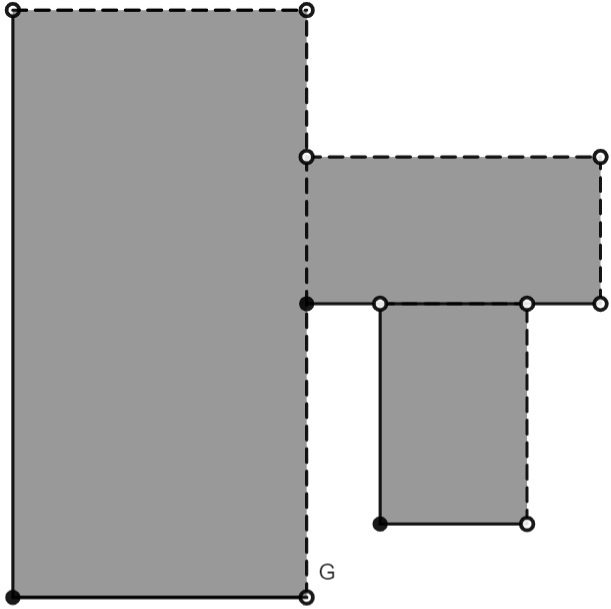
\includegraphics[scale = 0.3]{G(клет).jpg} \\ G - клеточное множество}
		\end{minipage}
		\hfill
		\begin{minipage}[h]{0.5\linewidth}
			\center{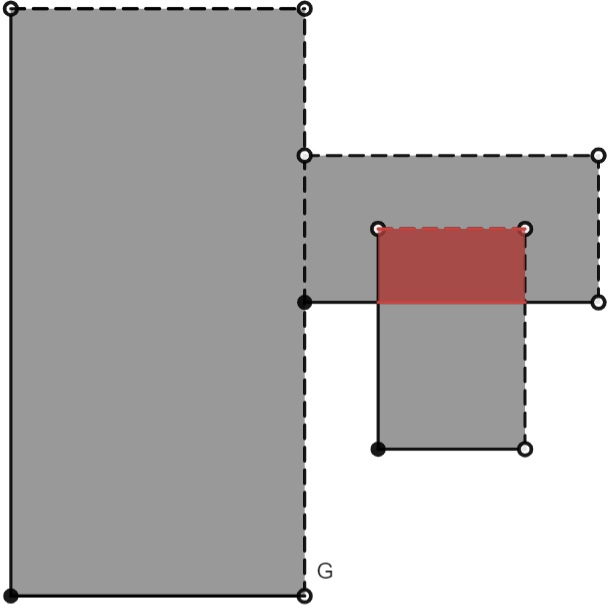
\includegraphics[scale = 0.3]{G(неклет).jpg} \\ G - не клеточное множество}
		\end{minipage}
	\end{figure}
	
	\textbf{Свойства клеточных множеств:}
	
	$\textbf{1}^\circ$ Объединение \textbf{конечного} числа попарно непересекающихся клеточных множеств есть клеточное множество.
	
	\textbf{Доказательство:}
	
	$G$ и $H$ - клеточные множества. Тогда:
	\begin{equation*}
		G = \bigcup_{j = 1}^k Q_j, \hspace{20mm} H = \bigcup_{j = k + 1}^n Q_j.
	\end{equation*}
	
	Значит:
	\begin{equation*}
		G \cup H = \bigcup_{j = 1}^n Q_j - \text{клеточное множество}.
	\end{equation*}
	
	$\textbf{2}^\circ$ Пересечение двух клеток есть клетка.
	
	\textbf{Доказательство:} 
	
	Пусть $Q_1 = [a_1, b_1) \times [a_2, b_2) \times \dots \times [a_m, b_m)$, а $Q_2 = [c_1, d_1) \times [c_2, d_2) \times \dots \times [c_m, d_m)$. Тогда возможны два случая:
	
	а) $\exists j$: $[a_j, b_j) \cap [c_j, d_j) = \varnothing \Rightarrow Q_1 \cap Q_2 = \varnothing $ - клетка;
	
	б) $\forall j \longmapsto [a_j, b_j) \cap [c_j, d_j) = [e_j, f_j) \Rightarrow Q_1 \cap Q_2 = [e_1, f_1) \times [e_2, f_2) \times \ldots \times [e_m, f_m)$ - клетка.
	
	\vspace{5mm}
	
	$\textbf{3}^\circ$ Пересечение двух клеточных множеств есть клеточное множество.
	
	\textbf{Доказательство:}
	
	Пусть $G_1$ и $G_2$ - клеточные множества.
	
	$G_1 = Q_1^1 \cup Q_2^1 \cup \ldots \cup Q_k^1$
	
	$G_2 = Q_1^2 \cup Q_2^2 \cup \ldots \cup Q_n^2$
	
	Обозначим $Q_{ij} = Q_i^1 \cap Q_j^2, \text{ } i = \overline{1, k}, \text{ } j = \overline{1, n}.$
	
	$Q_{ij}$ - клетка (свойство $\textbf{2}^\circ$).
	
	$G_1 \cap G_2 = \bigcup\limits_{i, j} Q_{ij} = \bigcup\limits_{i = 1}^k \bigcup\limits_{j = 1}^n Q_{ij}$ - объединение попарно непересекающихся клеток есть клеточное множество.
	
	\vspace{5mm}
	
	$\textbf{4}^\circ$ Разность двух клеток есть клеточное множество.
	
	\textbf{Доказательство:}
	
	$Q_1$ и $Q_2$ - клетки. $Q = Q_1 \cap Q_2$ - клетка (свойство $\textbf{2}^\circ$). Тогда
	
	$Q_1 \backslash Q_2 = Q_1 \backslash Q$.
	
	Существует такое разбиение клетки $Q_1$ на более мелкие клетки, что $Q$ является одной из них
	$\Rightarrow Q_1 \backslash Q_2$ - клеточное множество.
	
	\begin{figure}[h!]
		\centering
		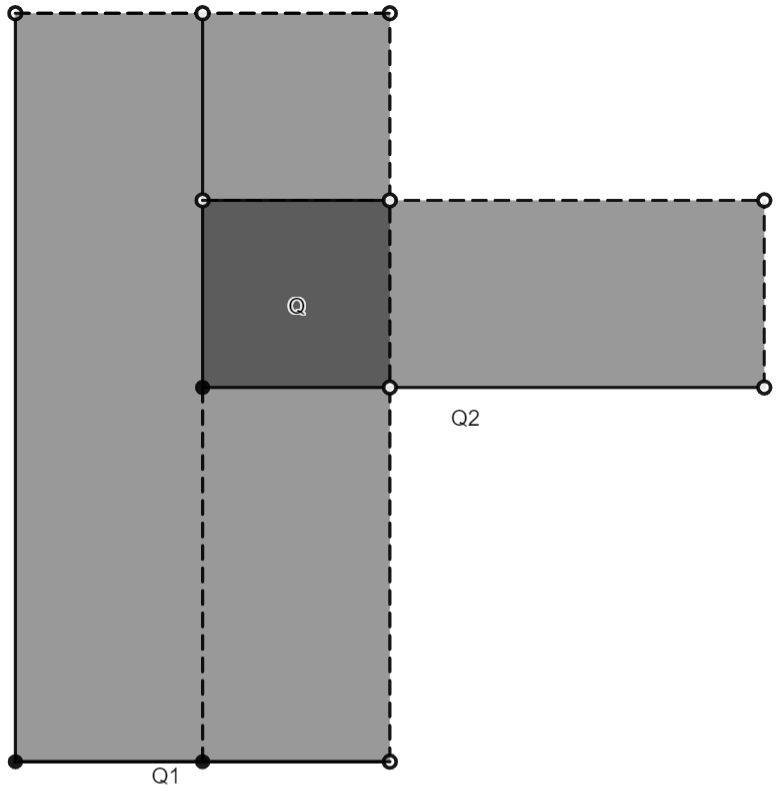
\includegraphics[scale=0.1]{Q.jpg}
	\end{figure} 
	
	
	
	$\textbf{5}^\circ$ Разность двух клеточных множеств есть клеточное множество.
	
	\textbf{Доказательство:}
	
	\begin{equation*}
		G_1 = \bigcup_{j = 1}^k Q_j^1, \hspace{20mm} G_2 = \bigcup_{j = 1}^n Q_j^2.
	\end{equation*}
	
	
	\begin{equation*}
		G_1 \backslash Q_1^2 = \bigcup_{i = 1}^k \left(Q_i^1 \backslash Q_1^2\right) = \bigcup_{i = 1}^k G_{i1} 
	\end{equation*}
	
	
	$G_{i1}$ - клеточное множество (свойство $\textbf{4}^\circ$).
	
	$G_{i1} \cap G_{j1} = \varnothing$, если $i \neq j \Rightarrow G_1 \backslash Q_1^2$ - клеточное множество (свойство $\textbf{1}^\circ$). 
	
	Аналогично для других клеток $G_2$
	
	\begin{equation*}
		G_1 \backslash G_2 = G_1 \backslash \left( \bigcup_{j = 1}^n Q_j^2\right) = \bigcap_{j = 1}^n\left(G_1 \backslash Q_j^2\right)
	\end{equation*}
	
	Последнее является клеточным множеством по свойству $\textbf{3}^\circ$. Откуда получаем, что $G_1\backslash G_2$ - клеточное множество.
	
	\vspace{5mm}
	
	$\textbf{6}^\circ$ Объединение \textbf{конечного} числа клеточных множеств есть клеточное множество.
	
	\textbf{Доказательство:}
	
	1) $G_1$ и $G_2$.
	
	$G_1 \cup G_2 = \left(G_1 \backslash G_2\right) \cup \left(G_2 \backslash G_1\right) \cup \left(G_1 \cap G_2\right)$;
	
	Последние три скобки являются попарно непересекающимися клеточными множествами $\stackrel{\textbf{1}^\circ}{\Rightarrow}$ $G_1 \cup G_2$ - клеточное множество.
	
	2) Далее для $G_3, G_4, \ldots, G_n$ по индукции.
	
	\vspace{7mm}
	
	\textbf{Таким образом, объединение, пересечение и разность конечного числа клеточных множеств есть клеточное множество.}
	
	\vspace{7mm}
	
	\underline{\textbf{Определение:}} мерой клетки $Q$ назовем число:
	
	$m(Q) = (b_1 - a_1)\cdot (b_2 - a_2)\cdot\ldots\cdot (b_m - a_m)$;
	
	$m(\varnothing) = 0$.\\
	
	\underline{\textbf{Определение:}} мерой клеточного множества $G$ назовем число:
	\begin{equation*}
		m(G) = \sum\limits_{j = 1}^{k} m(Q_j); \hspace{20mm} m(\varnothing) = 0.
	\end{equation*}
	
	\underline{\textbf{Лемма:}} мера клеточного множества $G$ не зависит от способа разбиения этого множества на клетки.\\
	
	\textbf{Доказательство:}
	
	Пусть $G = Q_1 \cup Q_2 \cup \ldots \cup Q_k$ и также $G = Q'_1 \cup Q'_2 \cup \ldots \cup Q'_n$. Тогда обозначим $Q_{ij} = Q_i \cap Q'_j, \text{ } i = \overline{1, k}, \text{ } j = \overline{1, n}.$
	
	Понятно, что 
	\begin{equation*}
		Q_i = \bigcup_{j = 1}^n Q_{ij}, \hspace{20mm} Q'_j = \bigcup_{i = 1}^k Q_{ij}.
	\end{equation*}
	
	Тогда:
	
	\begin{equation*}
		m(G) =  \sum\limits_{i = 1}^{k} m(Q_i) = \sum\limits_{i = 1}^{k} \sum\limits_{j = 1}^{n} m(Q_{ij}) = \sum\limits_{j = 1}^{n} \sum\limits_{i = 1}^{k} m(Q_{ij}) = \sum\limits_{j = 1}^{n} m(Q'_j) = m(G).
	\end{equation*}
	
	\underline{\textbf{Предложение 1:}} если клеточные множества $G_1, G_2, \ldots, G_n$ попарно не пересекаются, то для $G = \bigcup\limits_{j = 1}^n G_j$ выполняется $m(G) = \sum\limits_{j = 1}^n m(G_j)$.\\
	
	\textbf{Доказательство:}
	
	$G_j = \bigcup\limits_{i = 1}^{k_j} Q_i^j, \text{ } j = \overline{1, n}.$
	
	Тогда
	
	$G = \bigcup\limits_{j = 1}^n G_j = \bigcup\limits_{j = 1}^n \bigcup\limits_{i = 1}^{k_j} Q_i^j = \bigcup\limits_{\substack{1 \leqslant j \leqslant n,\\ 1\leqslant i \leqslant k_j}} Q_i^j$
	
	Все клетки из последнего объединения попарно не пересекаются, поэтому:
	
	$m(G) = \sum\limits_{\substack{1 \leqslant j \leqslant n,\\ 1\leqslant i \leqslant k_j}} m(Q_i^j) = \sum\limits_{j = 1}^n m(G_j)$.
	
	\vspace{5mm}
	
	\underline{\textbf{Предложение 2:}} если $G_1$ и $G_2$ - клеточные множества и $G_1 \subset G_2$, то $m(G_2) = m(G_1) + m(G_2 \backslash G_1)$,  $m(G_1) \leqslant m(G_2)$.\\
	
	\textbf{Доказательство:}
	
	$G_2 = G_1 \cup (G_2 \backslash G_1) = G_1 \cup G$.
	
	$G_1 \cap G = \varnothing \stackrel{\text{пр.1}}{\Longrightarrow} m(G_2) = m(G_1) + m(G_2 \backslash G_1) \Rightarrow m(G_1) \leqslant m(G_2)$.
	
	\underline{\textbf{Предложение 3:}} если $G_1, G_2, \ldots, G_k$ - клеточные множества, $G = \bigcup\limits_{j = 1}^k G_j$, то $m(G) \leqslant \sum\limits_{j = 1}^k m(G_j)$.
	
	\textbf{Доказательство:}
	
	Для $G_1$ и $G_2$ по предложению 2, а далее по индукции.
	
	\vspace{3mm}
	
	\underline{\textbf{Предложение 4:}} для любого клеточного множества $G$ и $\forall \varepsilon > 0$ $\exists G_{\varepsilon}, G^{\varepsilon}$ - клеточные множества такие, что:
	
	1) $G_{\varepsilon} \subset \overline{G_{\varepsilon}} \subset \text{int } G \subset G$;\hspace{8mm} $m(G) - m(G_{\varepsilon}) < \varepsilon$;
	
	2) $G \subset \overline{G} \subset \text{int } G^{\varepsilon} \subset G^{\varepsilon}$; \hspace{7mm} $m(G^{\varepsilon}) - m(G) < \varepsilon$.\\
	
	\textbf{Доказательство:}
	
	1) $G = Q_1 \cup Q_2 \cup \ldots \cup Q_k$.
	
	Рассмотрим отдельную клетку $Q = [a_1, b_1) \times [a_2, b_2) \times \ldots \times [a_m, b_m)$
	
	\begin{figure}[h!]
		\centering
		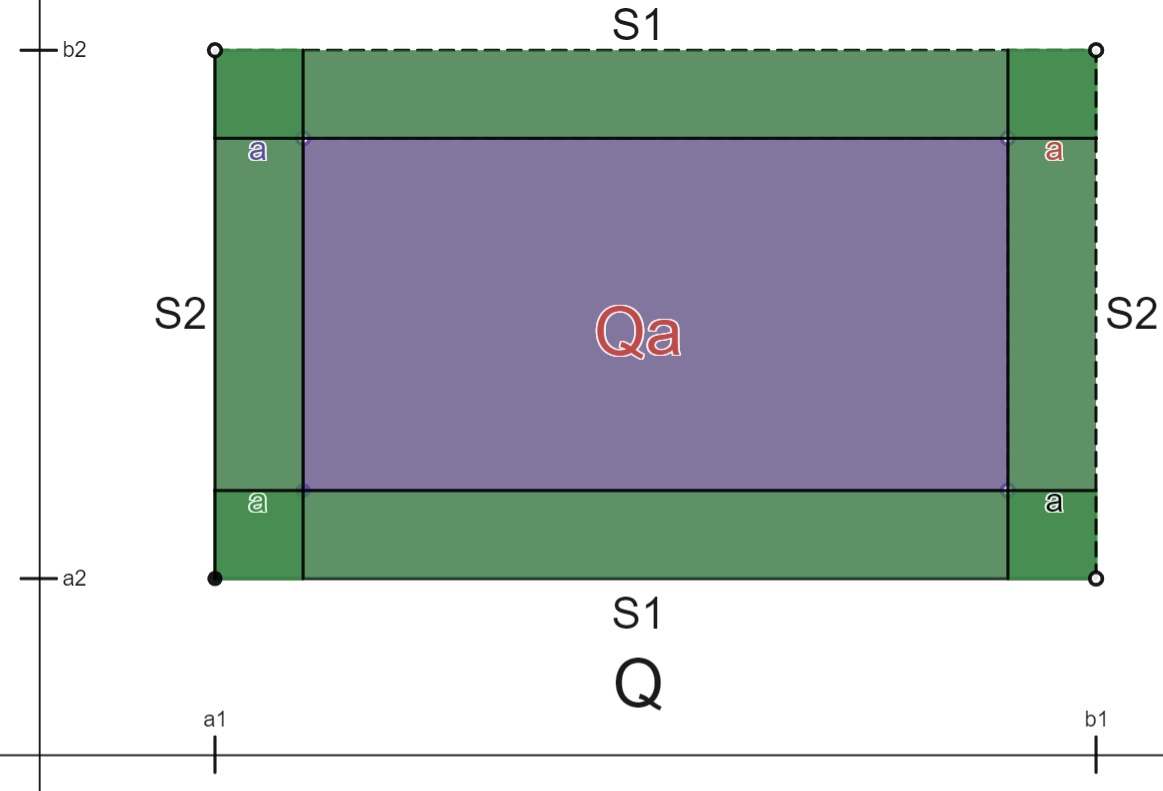
\includegraphics[scale=0.3]{Пред4.jpg}
		\caption{Случай при $m$ = 2}
	\end{figure}
	
	\[m(Q_a) = \prod\limits_{j = 1}^m (b_j - a_j - 2a) \text{, }  Q_a \subset Q \]
	\[S_j = \prod\limits_{\substack{i = 1,\\ i \neq j}}^m (b_i - a_i);\]
	
	Тогда
	\[m(Q) \leqslant m(Q_a) + 2a\cdot\sum\limits_{j = 1}^m S_j = m(Q_a) + 2aS \Rightarrow m(Q) - m(Q_a) \leqslant 2aS = \frac{\varepsilon}{2} < \varepsilon \]
	
	Тогда для одной клетки $a = \frac{\varepsilon}{4S}$.
	
	Так как $G = Q_1 \cup Q_2 \cup \ldots \cup Q_k$, то $a = \frac{\varepsilon}{4Sk}$.
	
	Получаем $G_{\varepsilon} = \bigcup\limits_{i = 1}^k (Q_a)_i$.
	
	Таким образом, $G_{\varepsilon} \subset \overline{G_{\varepsilon}} \subset \text{int } G \subset G$.
	
	\vspace{3mm}
	2) Доказывается аналогично 1).\\
	
	
	\subsection{Определение измеримости по Жордану множества в $m$-мерном евклидовом пространстве.}
	
	\underline{\textbf{Определение:}} множество $X \subset \mathbb{E}^m$ называется измеримым по Жордану, если $\forall \varepsilon > 0 \text{ }\exists G_{\varepsilon}$ и $G^{\varepsilon}$ - клеточные множества такие, что $G_{\varepsilon} \subset X \subset G^{\varepsilon}$ и $m(G^{\varepsilon}) - m(G_{\varepsilon}) < \varepsilon$. 
	
	\vspace{3mm}
	
	\underline{\textbf{Определение:}} мерой измеримого по Жордану множества $X \subset \mathbb{E}^m$ называется такое число $m(X)$, что $\forall G_{\varepsilon},\text{ } G^{\varepsilon}$ таких, что $G_{\varepsilon} \subset X \subset G^{\varepsilon} \longmapsto m(G_{\varepsilon}) \leqslant m(X) \leqslant m(G^{\varepsilon})$.
	
	\vspace{3mm}
	
	\underline{\textbf{Лемма:}} для любого измеримого по Жордану множества $X$ его мера $m(X)$ существует и единственна, причем
	
	\begin{equation*}
		m(X) = \overline{m}(X) = \underline{m}(X),
	\end{equation*}
	
	\noindent где $\overline{m}(X) = \inf\limits_{X \subset G^{\varepsilon}} m(G^{\varepsilon})$ - верхняя (внешняя) мера $X$;
	
	\noindent $\underline{m}(X) = \sup\limits_{G_{\varepsilon} \subset X} m(G_{\varepsilon})$ - нижняя (внутренняя) мера $X$.\\
	
	\textbf{Доказательство:} 
	
	Так как $G_{\varepsilon} \subset X \subset G^{\varepsilon}$, то $m(G_{\varepsilon}) \leqslant m(G^{\varepsilon}) \Rightarrow$ $\{m(G_{\varepsilon})\}$ ограничена сверху $\Rightarrow$
	
	$\Rightarrow$ $\exists \alpha = \sup\limits_{G_{\varepsilon}} m(G_{\varepsilon}) = \underline{m}(X)$.
	
	Аналогично: $\{m(G^{\varepsilon})\}$ ограничена снизу $\Rightarrow$ $\exists \beta = \inf\limits_{G^{\varepsilon}} m(G^{\varepsilon}) = \overline{m}(X)$.
	
	\vspace{3mm}
	
	По теореме об отделимости множеств: $m(G_{\varepsilon}) \leqslant \alpha \leqslant \beta \leqslant m(G^{\varepsilon})$.
	
	\vspace{3mm}
	Пусть $m(X) = \alpha$.
	
	$\forall \varepsilon > 0$ $\longmapsto$ $0 \leqslant \beta - \alpha \leqslant m(G^{\varepsilon}) - m(G_{\varepsilon}) < \varepsilon$.
	
	Откуда $\beta = \alpha$ $\Rightarrow m(X)$ единственна. 
	
	
	\vspace{3mm}
	
	\underline{\textbf{Предложение 5:}} пусть множество $X$ измеримо по Жордану и $\forall \varepsilon > 0$ $\exists G^{\varepsilon}$: $X \subset G^{\varepsilon}$, $m(G^{\varepsilon}) < \varepsilon$. Тогда $m(X) = 0$.\\
	
	\textbf{Доказательство:} 
	
	Возьмем $G_{\varepsilon} = \varnothing$. Тогда:
	
	$\forall \varepsilon > 0 \longmapsto G_{\varepsilon} \subset X \subset G^{\varepsilon} \text{ } \& \text{ } m(G^{\varepsilon}) - m(G_{\varepsilon}) = m(G^{\varepsilon}) < \varepsilon \text{ } \Rightarrow$ 
	
	$\Rightarrow 0 \leqslant m(X) < \varepsilon \text{ } \Rightarrow m(X) = 0$.
	
	\vspace{3mm}
	
	\textbf{Замечание:} измеримое по Жордану множество, обладающее свойством из предыдущего предложения, будем называть множеством меры нуль.
	
	\vspace{3mm}
	
	\underline{\textbf{Предложение 6:}} подмножество множества меры нуль есть множество меры нуль.\\
	
	\textbf{Доказательство:}
	
	Пусть $m(X) = 0$ и $Y \subset X$. Тогда $\forall \varepsilon > 0 \text{ }\exists G^{\varepsilon}: X \subset G^{\varepsilon}, m(G^{\varepsilon}) < \varepsilon$.
	
	Как следствие:
	
	$\forall \varepsilon > 0 \text{ }\exists G^{\varepsilon}: Y\subset X \subset G^{\varepsilon}, m(G^{\varepsilon}) < \varepsilon$ $\Rightarrow m(Y) = 0$.
	
	\vspace{3mm}
	
	\underline{\textbf{Предложение 7:}} объединение конечного числа множеств меры нуль есть множество меры нуль.\\
	
	\textbf{Доказательство:}
	
	$m(X_1) = m(X_2) = 0$.
	
	$\forall \varepsilon > 0 \text{ }\exists G_1^{\varepsilon}: X_1 \subset G_1^{\varepsilon}, m(G_1^{\varepsilon}) < \frac{\varepsilon}{2}$;
	
	$\hspace{16mm}\exists G_2^{\varepsilon}: X_2 \subset G_2^{\varepsilon}, m(G_2^{\varepsilon}) < \frac{\varepsilon}{2}$.
	
	Тогда $X_1 \cup X_2 \subset G_1^{\varepsilon} \cup G_2^{\varepsilon} = G^{\varepsilon}$.
	
	$m(G^{\varepsilon}) \stackrel{\text{пр.3}}{\leqslant} m(G_1^{\varepsilon}) + m(G_2^{\varepsilon}) < \frac{\varepsilon}{2} + \frac{\varepsilon}{2} = \varepsilon \Rightarrow$ $m(X_1 \cup X_2) = 0$.
	
	Далее по индукции.\\
	
	\subsection{Критерий измеримости.}
	
	\underline{\textbf{Теорема [Критерий измеримости]:}}
	
	\begin{equation*}
		\left[X - \text{измеримо по Жордану}\right] \Longleftrightarrow \left[ X \text{ ограничено и } m(\partial X) = 0\right].
	\end{equation*}	
	
	\textbf{Доказательство:}
	
	$\Longrightarrow$:
	
	$X$ - измеримо по Жордану: $\forall \varepsilon > 0$ $\exists G_{\varepsilon}, G^{\varepsilon}$: $G_{\varepsilon} \subset X \subset G^{\varepsilon}$, \\$m(G^{\varepsilon}) - m(G_{\varepsilon}) < \frac{\varepsilon}{3}$;
	
	\vspace{2mm}
	
	Из предложения 4 $\Rightarrow$ $\exists \widetilde{G}^{\varepsilon}$: $\overline{G^{\varepsilon}} \subset \text{int } \widetilde{G^{\varepsilon}} \subset \widetilde{G^{\varepsilon}}$, $m(\widetilde{G^{\varepsilon}}) - m(G^{\varepsilon}) < \frac{\varepsilon}{3}$;
	
	$\exists \widetilde{G_{\varepsilon}}$: $\overline{\widetilde{G_{\varepsilon}}} \subset \text{int } G_{\varepsilon} \subset G_{\varepsilon}$, $m(G_{\varepsilon}) - m(\widetilde{G_{\varepsilon}}) < \frac{\varepsilon}{3}$.
	
	\vspace{2mm}
	
	Тогда: 
	
	$m(\widetilde{G^{\varepsilon}}) - m(\widetilde{G_{\varepsilon}}) = m(\widetilde{G^{\varepsilon}}) - m(G^{\varepsilon}) + m(G^{\varepsilon}) - m(G_{\varepsilon}) + m(G_{\varepsilon}) - m(\widetilde{G_{\varepsilon}}) < \frac{\varepsilon}{3} + \frac{\varepsilon}{3} + \frac{\varepsilon}{3}  = \varepsilon$.
	
	\vspace{2mm}
	
	$\widetilde{G_{\varepsilon}}$ не содержит точки $\partial X$, а $\widetilde{G^{\varepsilon}}$ содержит их все, откуда:
	
	$\widetilde{G^{\varepsilon}} \backslash \widetilde{G_{\varepsilon}}$ - клеточное множество и $\partial X \subset \widetilde{G^{\varepsilon}} \backslash \widetilde{G_{\varepsilon}}$
	
	$m(\widetilde{G^{\varepsilon}} \backslash \widetilde{G_{\varepsilon}}) = m(\widetilde{G^{\varepsilon}}) - m(\widetilde{G_{\varepsilon}}) < \varepsilon$ $\Rightarrow$ $m(\partial X) = 0$.\\
	
	
	$\Longleftarrow$:
	
	$X$ - ограничено $\Rightarrow$ $\exists Q$ - клетка: $X \subset Q$;
	
	\vspace{2mm}
	
	$\left[m(\partial X) = 0\right] \stackrel{\text{def}}{=} \left[\forall \varepsilon > 0 \text{ } \exists G^{\varepsilon}: \partial X \subset G^{\varepsilon}, m(G^{\varepsilon}) < \varepsilon\right]$ 
	
	\vspace{2mm}
	
	$Q \backslash G^{\varepsilon}$ - клеточное множество $\Rightarrow$ $ Q \backslash G^{\varepsilon} = \bigcup\limits_{j = 1}^k Q_j$, \hspace{7mm} где $Q_j$ не содержат точек $\partial X$.
	
	\begin{wrapfigure}{R}{0.4\textwidth}
		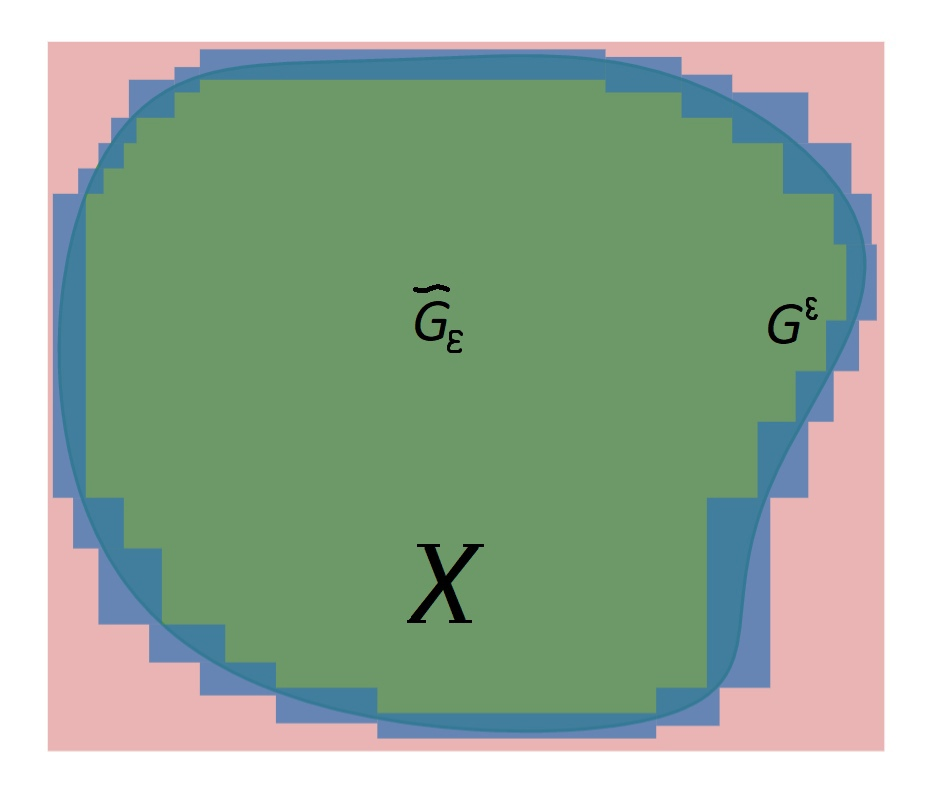
\includegraphics[scale=0.25]{Q(Клет).jpg}
	\end{wrapfigure}
	
	Тогда есть два варианта:
	
	$\left[Q_j \subset X\right]$ либо $\left[Q_j \cap X = \varnothing\right]$
	
	\vspace{2mm}
	
	Пусть без потери общности $Q_1, Q_2, \ldots, Q_l$: $\text{} Q_j \subset X$, $j = \overline{1,l}$;
	
	$Q_{l+1}, Q_{l+2}, \ldots, Q_k:\text{ } Q_j \cap X = \varnothing$, $j = \overline{l+1,k}$;
	
	
	\begin{equation*}
		\widetilde{G_{\varepsilon}} = \bigcup\limits_{j = 1}^l Q_j, \hspace{5mm} \widetilde{G^{\varepsilon}} = \widetilde{G_{\varepsilon}} \cup G^{\varepsilon} = Q \backslash \left(\bigcup\limits_{j = l + 1}^k Q_j\right)
	\end{equation*}
	
	
	$\widetilde{G_{\varepsilon}} \subset X \subset \widetilde{G^{\varepsilon}}$
	
	$m(G^{\varepsilon}) = m(\widetilde{G^{\varepsilon}}) - m(\widetilde{G_{\varepsilon}}) < \varepsilon \Rightarrow$ $X$ измеримо по Жордану.\\
	
	\subsection{Примеры неизмеримых по Жордану множеств.}
	
	\boxed{1} $X = \{x \in [0, 1]: x \in \mathbb{Q}\}, \text{ }X \subset \mathbb{E}^1$.
	
	$\partial X = [0,1] \Rightarrow m(\partial X) = 1 \neq 0$ $\Rightarrow X$ неизмеримо.
	
	\vspace{5mm}
	\boxed{2} $Y = X\times X$, где $X$ из \boxed{1}.
	
	$\partial Y = [0,1]\times [0,1] \Rightarrow$ $m(\partial Y) = 1 \neq 0$ $\Rightarrow Y$ неизмеримо.
	
	\vspace{5mm}
	\boxed{3} $X$ из \boxed{1}. $X = \{a_1, a_2, \ldots, a_n, \ldots\}$, $0 \leqslant a_j \leqslant 1$
	
	Пусть $B = \bigcup\limits_{j = 1}^{\infty} \left(a_j - \frac{\varepsilon}{2^j}; a_j + \frac{\varepsilon}{2^j}\right)$, $0 < \varepsilon < \frac{1}{2}$.
	
	$B$ открыто как объединение открытых множеств.
	
	Обозначим $B_k = \bigcup\limits_{j = 1}^k \left(a_j - \frac{\varepsilon}{2^j}; a_j + \frac{\varepsilon}{2^j}\right)$
	
	
	$m(B_k) \leqslant \sum\limits_{j = 1}^k \frac{\varepsilon}{2^{j-1}} = \varepsilon \left(\frac{1}{2} + \frac{1}{4} + \ldots + \frac{1}{2^{k-1}}\right) = \varepsilon \frac{1 - \frac{1}{2^k}}{\frac{1}{2}} = 2\varepsilon \left(1 - \frac{1}{2^k}\right) < 2\varepsilon$
	
	Тогда $\underline{m}(B) \leqslant 2\varepsilon < 1$. Но $[0, 1]\subset B \Rightarrow \overline{m}(B) > 1$.
	
	То есть $\underline{m}(B) \neq \overline{m}(B) \Rightarrow$  $B$ неизмеримо.\\
	
	\subsection{Измеримость объединения, пересечения и разности измеримых множеств.}
	
	$\textbf{1}^\circ$ Если $X_1$ и $X_2$ измеримы по Жордану, то $X_1 \cup X_2$, $X_1 \cap X_2$, $X_1 \backslash X_2$ - измеримые по Жордану множества.\\
	
	\textbf{Доказательство:}
	
	$X_1$ и $X_2$ измеримы по Жордану $\Rightarrow$ $X_1$ и $X_2$ ограничены и $m(\partial X_1) = m(\partial X_2) = 0$. Тогда и $m(\partial X_1 \cup \partial X_2) = 0$.
	\vspace{3mm}
	
	\noindent $\underbrace{\partial (X_1 \cup X_2) \subset \partial X_1 \cup \partial X_2;\text{ } \partial (X_1 \cap X_2) \subset \partial X_1 \cup \partial X_2;\text{ } \partial (X_1 \backslash X_2) \subset \partial X_1 \cup \partial X_2}_{\Downarrow}$	
	
	$m(\partial (X_1 \cup X_2)) = m(\partial (X_1 \cap X_2)) = m(\partial (X_1 \backslash X_2)) = 0 \Rightarrow$
	
	\vspace{2mm}
	\noindent $\Rightarrow X_1 \cup X_2, X_1 \cap X_2$ и $ X_1 \backslash X_2$ измеримы.\\
	
	
	\subsection{Конечная аддитивность меры Жордана.}
	
	$\textbf{2}^\circ$ Пусть $X_1, X_2, \ldots, X_k$ - измеримые по Жордану множества, тогда множество $X = \bigcup\limits_{j = 1}^k X_j$ измеримо и:
	
	1) $m(X) \leqslant \sum\limits_{j = 1}^k m(X_j)$;
	
	2) Если $X_j \cap X_i = \varnothing$ при $i \neq j$, то $m(X) = \sum\limits_{j = 1}^k m(X_j)$.
	
	\textbf{Доказательство:} (для $k = 2$, а дальше по индукции)
	
	\vspace{2mm}
	
	1) $X_1$ и $X_2$ измеримы по Жордану $\Rightarrow X = X_1 \cup X_2$ измеримо.
	
	$\forall \varepsilon > 0$ $\exists G_1^{\varepsilon}, G_2^{\varepsilon}$: $X_1 \subset G_1^{\varepsilon}$, $X_2 \subset G_2^{\varepsilon}$ и: 
	
	$m(X_1) > m(G_1^{\varepsilon}) - \frac{\varepsilon}{2}$
	
	$m(X_2) > m(G_2^{\varepsilon}) - \frac{\varepsilon}{2}$
	
	\vspace{2mm}
	
	Тогда $G^{\varepsilon} = G_1^{\varepsilon} \cup G_2^{\varepsilon}$ - клеточное множество и $X \subset G^{\varepsilon}$.
	
	Получаем:
	
	$m(X) \leqslant m(G^{\varepsilon}) \leqslant m(G_1^{\varepsilon}) + m(G_2^{\varepsilon}) < m(X_1) + m(X_2) + \varepsilon$.
	
	\vspace{2mm}
	
	В силу произвольности $\varepsilon \Rightarrow$ $m(X) \leqslant m(X_1) + m(X_2) \hspace{42mm} \boxed{*}$
	
	\vspace{5mm}
	2) $X_1 \cap X_2 = \varnothing$, $X = X_1 \cup X_2$
	
	$\forall \varepsilon > 0$ $\exists G_{\varepsilon}^1, G_{\varepsilon}^2$: $G_{\varepsilon}^1 \subset X_1$, $G_{\varepsilon}^2 \subset X_2$ и:
	
	$m(G_{\varepsilon}^1) > m(X_1) - \frac{\varepsilon}{2}$
	
	$m(G_{\varepsilon}^2) > m(X_2) - \frac{\varepsilon}{2}$
	
	\vspace{2mm}
	
	$G_{\varepsilon} = G_{\varepsilon}^1 \cup G_{\varepsilon}^2$ и $G_{\varepsilon}^1 \cap G_{\varepsilon}^2 = \varnothing$, а также $G_{\varepsilon}^1 \cup G_{\varepsilon}^2 \subset X$.
	
	\vspace{2mm}
	
	Тогда $m(X) \geqslant m(G_{\varepsilon}) = m(G_{\varepsilon}^1) + m(G_{\varepsilon}^2) > m(X_1) + m(X_2) - \varepsilon$.
	
	\vspace{2mm}
	
	В силу произвольности $\varepsilon > 0$ получаем $m(X) \geqslant m(X_1) + m(X_2) \hspace{16mm} \boxed{**}$ 
	
	\vspace{2mm}
	
	Из $\boxed{*}$ и $\boxed{**}$ $\Rightarrow$ $m(X) = m(X_1) + m(X_2)$.\\
	
	\subsection{Измеримость и мера цилиндра в $(m+1)$-мерном пространстве.}
	
	\underline{\textbf{Предложение:}} пусть $X \subset \mathbb{E}^m$, $m \geqslant 1$, - измеримо, тогда множество $Y = X\times [a, b) \subset \mathbb{E}^{m + 1}$ - измеримо. $m(Y) = m(X)(b - a)$.\\
	
	\textbf{Доказательство:}
	
	$\left[X \text{ измеримо}\right] \stackrel{\text{def}}{=} \left[\forall \varepsilon > 0\text{ }\exists G_{\varepsilon}, G^{\varepsilon}: G_{\varepsilon}\subset X\subset G^{\varepsilon}, \text{ } m(G^{\varepsilon}) - m(G_{\varepsilon}) < \frac{\varepsilon}{b - a}\right]$.
	
	\vspace{2mm}
	
	Рассмотрим клеточные множества: $\widetilde{G_{\varepsilon}} = G_{\varepsilon}\times [a, b)$ и $\widetilde{G^{\varepsilon}} = G^{\varepsilon}\times [a, b)$;
	
	\vspace{2mm}
	
	Тогда $\widetilde{G_{\varepsilon}} \subset Y \subset \widetilde{G^{\varepsilon}}$, а $m(\widetilde{G_{\varepsilon}}) = m(G_{\varepsilon})(b-a)$ и $m(\widetilde{G^{\varepsilon}}) = m(G^{\varepsilon})(b-a)$;
	
	Получаем: $m(\widetilde{G^{\varepsilon}}) - m(\widetilde{G_{\varepsilon}}) = (m(G^{\varepsilon}) - m(G_{\varepsilon}))(b-a) < \frac{\varepsilon}{b-a}(b-a) = \varepsilon$ $\Rightarrow Y$ измеримо.
	
	%=======================================================================================
	
	%БИЛЕТ 6
	%=======================================================================================
	
	\newpage
	\section{Билет 6}
	
	\subsection{Определенный интеграл Римана.}
	\underline{\textbf{Обозначения}}:
	
	$y = f(x)$ некоторая функция, $x \in [a,b]\\T$ -- разбиение отрезка $[a,b]: T = \{a = x_0 < x_1 < {\dots} < x_n = b \}\\\Delta x_j = x_j - x_{j-1},~\Delta_T = \max\limits_{1\leq j\leq n}\Delta x_j$ -- мелкость разбиения\\ $\xi_j \in [x_{j-1},x_j],~j = \overline{1,n}$\\
	
	\underline{\textbf{Определение:}} Число $I\{T,\xi\} =  \sum\limits_{j = 1}^{n} {f(\xi_j)\Delta x_j}$ называется интегральной суммой.\\
	
	\underline{\textbf{Определение:}} Число $I$ называется пределом интегральных сумм $I\{T,\xi\}$ при $\Delta_T \longrightarrow 0$, Если $\forall\varepsilon>0~\exists\delta = \delta(\varepsilon)>0: \forall T:\Delta_{T}<\delta~\&~ \forall\{\xi\} \longmapsto|I\{T, \xi\}-I|<\varepsilon$.\\
	
	\underline{\textbf{Определение:}} Функция $y = f(x)$ называется интегрируемой на $[a,b]$, если существует конечный предел $I$ интегральных сумм $I\{T,\xi\}$\\ при $\Delta_T \longrightarrow 0$.\\
	Указанный предел $I$ называется определенным интегралом функции $f$ на $[a,b]$.\\
	
	\underline{\textbf{Обозначение}}: $I = \int\limits_{a}^{b} {f(x)dx}$\\
	
	\textbf{Пример}: $y(x)\equiv C,~x\in[a,b]\\
	I\{T,\xi\} = C(b-a) \Rightarrow I = \int\limits_{a}^{b} {Cdx} = C(b-a)$\\
	
	\underline{\textbf{Предложение:}}[Необходимое условие интегрируемости функции]:
	
	\[ [f \text{ -- интегрируема на }[a,b]~] \, \Rightarrow[ f \text{ -- ограничена на }[a,b] ] \]
	
	\textbf{Доказательство}: от противного:
	\\
	Пусть $f$ не является ограниченной на $[a,b]$ это означает, что $\exists k:$ на $[x_{k-1},x_k]$
	функция не является ограниченной, то есть, $|f(\xi_k)|\Delta x_k$ может быть как угодно большим за счет выборки точки $\xi_k~\Rightarrow I\{T,\xi\}$ неограчена и предел $I\{T,\xi\}~\Delta_T\rightarrow 0$ не существует -- противоречие.\\
	
	\textbf{Замечание}: Не всякая ограниченная функция является интегрируемой на отрезке.\\
	
	\textbf{Пример}: функция Дирихле на любом отрезке $[a,b]$ ограничена
	$$y=D(x)=\left\{\begin{array}{ll}
		1, & x \in \mathbb{Q} \\
		0, & x \in \mathbb{J}
	\end{array}\right.$$
	
	Однако:
	
	$$\xi_j^{\prime} \in \mathbb{Q},~j = \overline{1,n}$$
	
	$$\xi_j^{\prime \prime} \in \mathbb{J},~j = \overline{1,n}$$
	
	$$I\{T,\xi^{\prime}\} = b-a\neq 0$$
	
	$$I\{T,\xi^{\prime \prime}\} = 0 \text{, отсюда } D(x) \text{ не является интегрируемой}$$
	
	\subsection{Верхние и нижние суммы Дарбу, их свойства.}
	
	\underline{\textbf{Определение:}} Пусть $y = f(x),~x\in [a,b]$, ограничена на данном отрезке; T--разбиение отрезка $[a,b]$.
	
	$ T = \{a = x_0 < x_1 < {\dots} < x_n = b\},~\Delta x_j = x_j - x_{j-1} $
	
	$m_j = \inf\limits_{[x_{j-1},x_j]}f(x),~M_j = \sup\limits_{[x_{j-1},x_j]}f(x),~j = \overline{1,n}$, тогда:\\
	
	$\underline{S}_T = \sum\limits_{j = 1}^{n}{m_j \Delta x_j}$--нижняя сумма Дарбу по разбиению T\\
	
	$\overline{S}_T = \sum\limits_{j = 1}^{n}{M_j \Delta x_j}$--верхняя сумма Дарбу по разбиению T\\
	
	Очевидно, что при фиксированном T выполняется $\underline{S}_T \leq  I\{T,\xi\} \leq \overline{S}_T$\\
	
	\textbf{Свойство 1}: Для фиксированного T выполняется:\\
	$\forall\varepsilon>0~\exists \xi^{\prime}, \xi^{\prime \prime}: \overline{S}_T - I\{T,\xi^{\prime}\}<\varepsilon,~I\{T,\xi^{\prime\prime}\}-\underline{S}_T<\varepsilon$\\
	
	\textbf{Доказательство}: из определения $M_j = \sup\limits_{[x_{j-1},x_j]}f(x)$\\
	$\forall\varepsilon>0~\exists \xi^{\prime}_j \in [x_{j-1},x_j]:~f(\xi^{\prime}_j)>M_j-\frac{\varepsilon}{b-a}~\Rightarrow~M_j-f(\xi^{\prime}_j)<\frac{\varepsilon}{b-a}$\\
	
	$\sum\limits_{j = 1}^{n} {(M_j-f(\xi^{\prime}_j))\Delta x_j}<\sum\limits_{j = 1}^{n} {\frac{\varepsilon}{b-a}\Delta x_j} = \varepsilon~\Rightarrow~\sum\limits_{j = 1}^{n} {(M_j-f(\xi^{\prime}_j))\Delta x_j}=\\$
	
	$\overline{S}_T - I\{T,\xi^{\prime}\}<\varepsilon$ \\
	Второе неравество доказывается аналогично.\\
	
	\underline{\textbf{Определение:}} $T^{\prime}$--измельчение разбиения $T$, если $T^{\prime}=T\cup \{b_1{\dots}b_k\}$, то есть, мы добавляем еще $k$ точек, таким образом $\Delta_{T^{\prime}}\leq \Delta_T$.\\
	
	\textbf{Свойство 2}: При измельчении разбиения $T$ нижние суммы Дарбу не уменьшаются, а верхние не увеличиваются.\\
	$T^{\prime}$--измельчение разбиения $T,~\underline{S}_T\leq \underline{S}_{T^{\prime}}\leq \overline{S}_{T^{\prime}}\leq \overline{S}_T$\\
	
	\textbf{Доказательство}: Добавим одну точку на $[x_{j-1},x_j]:~b\in (x_{j-1},x_j), \Delta x_j = \Delta x^{\prime}_j +\Delta x^{\prime\prime}_j,~M^{\prime}_j\leq M_j;~M^{\prime\prime}_j\leq M_j$, тогда:\\
	$$\overline{S}_T-\overline{S}_{T^{\prime}}=M_j\Delta x_j-(M^{\prime}_j\Delta x^{\prime}_j+M^{\prime\prime}_j\Delta x^{\prime\prime}_j)=(M_j-M^{\prime}_j)\Delta x^{\prime}+(M_j-M^{\prime\prime}_j)\Delta x^{\prime\prime}\geq0$$
	$\Rightarrow~\overline{S}_{T^{\prime}}\leq \overline{S}_T$\\
	Аналогично доказывается для нижних сумм.\\
	
	\textbf{Свойство 3}: Пусть $T^{\prime}$ и $T^{\prime\prime}$ произвольные разбиения отрезка $[a,b]$, тогда:
	$\underline{S}_{T^{\prime}}\leq \overline{S}_{T^{\prime\prime}},~\underline{S}_{T^{\prime\prime}}\leq \overline{S}_{T^{\prime}}$\\
	
	\textbf{Доказательство}: $T = T^{\prime}\cup T^{\prime\prime}$--измельчение разбиений $T^{\prime},~ T^{\prime\prime}$\\
	Тогда из свойства 2 следует, что $\underline{S}_{T^{\prime}}\leq \underline{S}_T\leq \overline{S}_T\leq \overline{S}_{T^{\prime\prime}}$ и\\
	$\underline{S}_{T^{\prime\prime}}\leq \underline{S}_T\leq \overline{S}_T\leq \overline{S}_{T^{\prime}}$\\
	
	
	\textbf{Свойство 4}: существуют числа $\underline{I},~\overline{I}$:\\
	$\underline{I}=\sup\limits_{T}{\underline{S}_T,~\overline{I}=\inf\limits_{T}{\overline{S}_T}}$ такие, что для произвольных разбиений $T^{\prime},~T^{\prime\prime}$ выполняется: 
	$\underline{S}_{T^{\prime}}\leq \underline{I}\leq \overline{I}\leq \overline{S}_{T^{\prime\prime}}$
	
	$\overline{I}$--верхний интеграл Дарбу
	
	$\underline{I}$--нижний интеграл Дарбу.\\
	
	\textbf{Доказательство}: следует из свойства 3 и теоремы об отделимости множеств.\\
	
	\underline{\textbf{Свойство 5 [Лемма Дарбу]}}:\\
	1)[$\underline{I}=\lim\limits_{\Delta_T\rightarrow 0}{\underline{S}_T}$] $\stackrel{\text { def }}{=}$ [$\forall\varepsilon>0~\exists\delta = \delta(\varepsilon)>0: \forall T:\Delta_{T}<\delta \longmapsto \underline{I}-\underline{S}_T<\varepsilon$]\\
	2)[$\overline{I}=\lim\limits_{\Delta_T\rightarrow 0}{\overline{S}_T}$] $\stackrel{\text { def }}{=}$ [$\forall\varepsilon>0~\exists\delta = \delta(\varepsilon)>0: \forall T:\Delta_{T}<\delta \longmapsto \overline{S}_T-\overline{I}<\varepsilon$]\\
	
	\textbf{Доказательство}: 2)\\
	$M=\sup\limits_{[a,b]}{f(x)},~m=\inf\limits_{[a,b]}{f(x)}$\\
	a)$M=m$ -- тривиальный случай;\\
	b)$M>m;~\overline{I}=\inf\limits_{T}{\overline{S}_T}$ из определения $inf$\\
	$\forall \varepsilon>0~\exists T^{*}:~\overline{S}_{T^{*}}<\overline{I}+\frac{\varepsilon}{2}~\Rightarrow~\overline{S}_{T^{*}}-\overline{I}<\frac{\varepsilon}{2}$\\
	$T$--произвольное разбиение: $\Delta_T=\max\limits_{j}{\Delta x_j}<\frac{\varepsilon}{2(M-m)k}$\\
	$k$--количество точек разбиения $T^{*}$, лежащих на $(a,b)$\\
	рассмотрим $T^{\prime}=T\cup T^{*}$\\
	$0\leq \overline{S}_T-\overline{S}_{T^{\prime}}\leq (M-m)k\Delta_T<\frac{\varepsilon}{2}$ (оценили сверху) отсюда:\\
	$0\leq \overline{S}_T-\overline{S}_{T^{\prime}}\leq \frac{\varepsilon}{2}$ (1)\\
	Из свойств 3 и 4: $\overline{I}\leq \overline{S}_{T^{\prime}}\leq  \overline{S}_{T^{*}}$\\
	$0\leq  \overline{S}_{T^{\prime}}-\overline{I}\leq \overline{S}_{T^{*}}-\overline{I}<\frac{\varepsilon}{2}~\Rightarrow$\\
	$\overline{S}_{T^{\prime}}-\overline{I}<\frac{\varepsilon}{2}$ (2)\\
	Складываем (1) и (2), получаем $ \overline{S}_T-\overline{I}<\varepsilon$\\
	Итак:$\forall \varepsilon>0 \quad \exists \delta=\delta(\varepsilon)=\frac{\varepsilon}{2(M-m) k}>0$
	$\forall T: \Delta_{T}<\delta \longmapsto\overline{S}_T-\overline{I}<\varepsilon$\\
	
	\subsection{Критерий интегрируемости функции.}
	
	
	\underline{\textbf{Теорема 1:}} Пусть функция $f$ ограничена на $[a,b]$\\
	$[\,f$ интегрируема на $[a,b]~]\, \Leftrightarrow [\,\forall\varepsilon>0~\exists T:~\overline{S}_T-\underline{S}_T<\varepsilon]\,$\\
	
	\textbf{Доказательство [Необходимость]}: $\Rightarrow$\\
	$[\,f$ интегрируема на $[a,b]~] \stackrel{\text{def}}{=}[\,\forall\varepsilon>0~\exists\delta=\delta(\varepsilon)>0: \forall T:\\\Delta_{T}<\delta~\&~ \forall\{\xi\} \longmapsto|I-I\{T, \xi\}|<\frac{\varepsilon}{4}]\,$\\
	из свойства 1: $\exists \xi^{\prime},~\xi^{\prime\prime}$:\\
	$ \overline{S}_T - I\{T,\xi^{\prime}\}<\frac{\varepsilon}{4},~I\{T,\xi^{\prime\prime}\}-\underline{S}_T<\frac{\varepsilon}{4}$, тогда\\
	$\overline{S}_T-\underline{S}_T=|\overline{S}_T-I\{T,\xi^{\prime}\}+I\{T,\xi^{\prime}\}-I+I-I\{T,\xi^{\prime\prime}\}+I\{T,\xi^{\prime\prime}\}-\underline{S}_T|\leq \overline{S}_T-I\{T,\xi^{\prime}\}+|I\{T,\xi^{\prime}\}-I|+|I-I\{T,\xi^{\prime\prime}\}|+I\{T,\xi^{\prime\prime}\}-\underline{S}_T<4\cdot \frac{\varepsilon}{4}=\varepsilon~\Rightarrow$\\
	$\forall\varepsilon>0~\exists T:~\overline{S}_T-\underline{S}_T<\varepsilon$\\
	
	\textbf{Доказательство [Достаточность]}: $\Leftarrow$\\
	$\forall\varepsilon>0~\exists T^{*}_{\varepsilon}:~\overline{S}_{T^{*}}-\underline{S}_{T^{*}}<\varepsilon$\\
	Из свойства 4: существуют числа $\underline{I},~\overline{I}:~\forall T\longmapsto \underline{S}_{T}\leq \underline{I}\leq \overline{I}\leq \overline{S}_{T}~\Rightarrow$\\
	$0\leq \overline{I}-\underline{I}\leq \overline{S}_{T^{*}}-\underline{S}_{T^{*}}<\varepsilon$ так как это выполняется для любых $\varepsilon>0~\Rightarrow$ это возможно лишь при $\overline{I}-\underline{I}=0$, $\overline{I}=\underline{I}=I$\\
	По Лемме Дарбу:\\
	$\forall\varepsilon>0~\exists\delta_1 = \delta_{1}(\varepsilon)>0: \forall T:\Delta_{T}<\delta_1 \longmapsto \overline{S}_T-\overline{I}<\varepsilon$\\
	для этого же $\varepsilon~\exists\delta_2 = \delta_{2}(\varepsilon)>0: \forall T:\Delta_{T}<\delta_2 \longmapsto \underline{I}-\underline{S}_T<\varepsilon$\\
	$\delta=min\{\delta_1,\delta_2\}\Rightarrow$
	$\forall T~\Delta_T<\delta \longmapsto$\\
	$\overline{S}_T-I<\frac{\varepsilon}{2},~I-\underline{S}_T<\frac{\varepsilon}{2}$\\
	$\forall T~\Delta_T<\delta~\&~\forall \xi=\{\xi_j\}\longmapsto$\\
	$\underline{S}_T\leq I\leq \overline{S}_T$ (1)\\
	также используем то, что $\underline{S}_T\leq I\{T,\xi\}\leq \overline{S}_T\Rightarrow$\\
	$-\overline{S}_T\leq -I\{T,\xi\}\leq -\underline{S}_T$ (2)\\
	Сложим (1) и (2) $\Rightarrow |I-I\{T,\xi\}|\leq \overline{S}_T-\underline{S}_T<\varepsilon$\\
	\subsection{Классы интегрируемых функций.}
	
	
	\underline{\textbf{Теорема 2:}} Если $y=f(x)$ непрерывна на отрезке $[a,b]$, то $f$ интегрирума на $[a,b]$.\\
	
	\textbf{Доказательство}: $f$ ограничена на $[a,b]$ по первой теореме Вейерштрасса, $f$ равномерно непрерывна на $[a,b]$ по теореме Кантора $\Rightarrow$\\
	$\forall\varepsilon>0~\exists\delta=\delta(\varepsilon)>0: \forall x^{\prime},~x^{\prime\prime} \in [a,b]:~|x^{\prime}-x^{\prime\prime}|<\delta \longmapsto\\|f(x^{\prime})-f(x^{\prime\prime})|<\frac{\varepsilon}{b-a}$\\
	Для этого же $\varepsilon~\exists T:~\Delta_T<\delta,~T=\{a=x_0<x_1<{\dots}<x_n=b\}$\\
	По 2 теореме Вейерштрасса $\forall j~\exists x^{\prime}_j,~x^{\prime\prime}_j\in [x_{j-1},x_j]:~\\
	M_j=\max\limits_{[x_{j-1},x_j]}{f(x)}=f(x^{\prime}_j),~m_j=\min\limits_{[x_{j-1},x_j]}{f(x)}=f(x^{\prime\prime}_j)$\\
	тогда из р.н. получаем, что $\forall j~M_j-m_j<\frac{\varepsilon}{b-a}\Rightarrow$\\
	$\overline{S}_T-\underline{S}_T=\sum\limits^{n}_{j=1}{(M_j-m_j)\Delta x_j}<\frac{\varepsilon}{b-a}\sum\limits^{n}_{j=1}{\Delta x_j}=\frac{\varepsilon(b-a)}{b-a}=\varepsilon\Rightarrow$\\
	$\forall\varepsilon>0~\exists T:~\overline{S}_T-\underline{S}_T<\varepsilon$.\\
	
	
	\underline{\textbf{Теорема 3:}} Если функция $y=f(x)$ определена на отрезке $[a,b]$ и монотонна на отрезке, то $f$ интегрируема на $[a,b]$.\\
	
	\textbf{Доказательство}: для неубывающей функции: $\forall x\in[a,b]\longmapsto\\
	f(a)\leq f(x) \leq f(b)\Rightarrow$ ограничена\\
	$\forall\varepsilon>0~\exists T:~\Delta_T<\frac{\varepsilon}{f(b)-f(a)},~T=\{a=x_0<x_1<{\dots}<x_n=b\}$\\
	$j=\overline{1,n}~[x_{j-1},x_j]\longmapsto
	M_j=f(x_j),~m_j=f(x_{j-1})$\\
	$\overline{S}_T-\underline{S}_T=\sum\limits^{n}_{j=1}{(M_j-m_j)\Delta x_j}<\frac{\varepsilon}{f(b)-f(a)}(f(x_1)-f(x_0)+f(x_2)-\\
	-f(x_1)+{\dots}+f(x_n)-f(x_{n-1}))=\frac{\varepsilon(f(b)-f(a))}{f(b)-f(a)}=\varepsilon\Rightarrow$\\
	$\forall\varepsilon>0~\exists T:~\overline{S}_T-\underline{S}_T<\varepsilon$\\
	
	\underline{\textbf{Теорема 4:}} Если функция $y=f(x)$ ограничена на $[a,b]$ и $\forall\varepsilon>0$ существует конечное число интервалов, покрывающих точки разрыва функции $f$, сумма длин которых не превосходит $\varepsilon\Rightarrow~f$ интегрируема на $[a,b]$\\
	
	\textbf{Доказательство}: Пусть $M=\sup\limits_{[a,b]}{f(x)},~m=\inf\limits_{[a,b]}{f(x)}$\\
	$\forall \varepsilon>0~\exists X_1=\bigcup\limits^{n}_{j=1}{\delta^{1}_j}$ -- интервал, покрывающий точки разрыва и $|\delta^{1}_j|$ -- его длина $\Rightarrow~\sum\limits^{n}_{j=1}{|\delta^{1}_j|}<\frac{\varepsilon}{2(M-m)}$\\
	$X_2=(a,b)\setminus\overline{X_1}$ \\
	$(a,b)$ -- открытое, $\overline{X_1}$ -- замкнутое $\Rightarrow~X_2$ -- открытое, то есть, мы отбросили интервалы с точками разрыва.\\
	$X_2=\bigcup \limits^{k}_{j=1}{\delta^{2}_j}$ на каждом $\delta^{2}_j$ -- $f$ непрерывна $\Rightarrow~f$ равномерно непрерывна на $\overline{X_2}$ (Замыкание, то есть $\overline{X_2}$ компакт -- ограниченное и замкнутое)\\
	
	Тогда из опр. р.н. $\exists\delta=\delta(\varepsilon)>0: \forall x^{\prime},~x^{\prime\prime} \in \overline{X_2}~ \longmapsto\\|f(x^{\prime})-f(x^{\prime\prime})|<\frac{\varepsilon}{2(b-a)}$, $T=\{\delta^{1}_j,~\delta^{2}_i\}^{n~~~~k}_{j=1,~i=1}$, то есть концы интервалов образует разбиение отрезка $[a, b]$.\\
	$\overline{S}_T-\underline{S}_T=\sum\limits^{n}_{j=1}{(M_j-m_j)|\delta^{1}_j|}+\sum\limits^{k}_{i=1}{(M_i-m_i)|\delta^{2}_i|}\leq(M-m)\sum\limits^{n}_{j=1}{|\delta^{1}_j|} 
	+\frac{\varepsilon}{2(b-a)}\sum\limits^{k}_{i=1}{|\delta^{2}_i|}<\frac{\varepsilon}{2}+\frac{\varepsilon(b-a)}{2(b-a)}=\varepsilon\Rightarrow \forall\varepsilon>0~\exists T:~\overline{S}_T-\underline{S}_T<\varepsilon\Rightarrow~f$ интегрируема на $[a,b]$.\\
	
	\textbf{Следствие}: Если функция $y=f(x)$ ограничена на $[a,b]$ и имеет на нем конечное число точек разрыва, то $f$ интегрируема на $[a,b]$\\
	
	Рассмотрим пример функции, имеющей на отрезке бесконечное число точек разрыва:\\
	
	\textbf{Пример}: $f(x)=\left\{\begin{array}{ll}~~1,~x \in\left(\frac{1}{2 n}, \frac{1}{2 n-1}\right], n \in \mathbb{N} \\ -1,~x \in\left(\frac{1}{2 n+1}, \frac{1}{2 n}\right], n \in \mathbb{N}\end{array}\right.$\\
	$$x\in[0,1]$$\\ 
	\begin{center}
		\begin{tikzpicture}
			\draw [white!90!black] (0.1, 0.1) grid (15.9, 9.9);
			\draw [->,>=stealth] (1, 5) -- (15, 5) node[below] {$x$};
			\draw [->,>=stealth] (2, 1) -- (2, 9) node[left] {$y$};
			\draw [dashed, white!60!black] (12, 5) -- (12, 8);
			\draw [dashed, white!60!black] (7, 2) -- (7, 8);
			\draw [dashed, white!60!black] (5.33, 2) -- (5.33, 8);
			\draw [dashed, white!60!black] (4.5, 2) -- (4.5, 8);
			\draw [dashed, white!60!black] (4, 2) -- (4, 8);
			\draw [dashed, white!60!black] (3.66, 2) -- (3.66, 8);
			\draw [dashed, white!60!black] (3.428, 2) -- (3.428, 5);
			\draw [dashed, white!60!black] (3.428, 2) -- (2, 2);
			\draw [dashed, white!60!black] (3.66, 8) -- (2, 8);
			\draw [fill=black] (2, 8) circle (2pt) node[left]{$1$};
			\draw [fill=black] (2, 2) circle (2pt) node[left]{$-1$};
			\draw [fill=black] (12, 5) circle (2pt) node[below]{$1$};
			\draw [fill=black] (7, 5) circle (2pt) node[below]{$\frac{1}{2}$};
			\draw [fill=black] (5.33, 5) circle (2pt) node[below]{$\frac{1}{3}$};
			\draw [fill=black] (4.5, 5) circle (2pt) node[below]{$\frac{1}{4}$};
			\draw [fill=black] (4, 5) circle (2pt) node[below]{$\frac{1}{5}$};
			\draw [fill=black] (3.66, 5) circle (2pt) node[below]{$\frac{1}{6}$};
			\draw [fill=black] (3.428, 5) circle (2pt) node[below]{$\frac{1}{7}$};
			\draw [->,>=stealth, line width=1.5] (12, 8) -- (7, 8);
			\draw [->,>=stealth, line width=1.5] (7, 2) -- (5.33, 2);
			\draw [->,>=stealth, line width=1.5] (5.33, 8) -- (4.5, 8);
			\draw [->,>=stealth, line width=1.5] (4.5, 2) -- (4, 2);
			\draw [->,>=stealth, line width=1.5] (4, 8) -- (3.66, 8);
			\draw [->,>=stealth, line width=1.5] (3.66, 2) -- (3.428, 2);
			\draw [fill=red] (2.7, 5) circle (2pt) node[below]{$\frac{\varepsilon}{4}$};
			\draw [fill=blue] (2.57, 5) circle (1pt);
			\draw [fill=blue] (2.47, 5) circle (1pt);
			\draw [fill=blue] (2.37, 5) circle (1pt);
			\draw [fill=blue] (2.27, 5) circle (1pt);
			\draw [fill=blue] (2.17, 5) circle (1pt);
			\draw [fill=blue] (2.07, 5) circle (1pt);
		\end{tikzpicture}\\    
	\end{center}
	
	Точки разрыва $\frac{1}{n},~n>1$ на $[0,1]$.
	
	$\forall\varepsilon>0~\exists N=N(\varepsilon):~\forall n\geq N\longmapsto 0<\frac{1}{n}<\frac{\varepsilon}{4}$
	
	Оставшиеся $N$ точек вне данного интервала покрываем интервалами длины $\frac{\varepsilon}{4N}$, тогда сумма длин итервалов покрытия равна $\frac{\varepsilon}{4}+N\frac{\varepsilon}{4N}=\frac{\varepsilon}{2}<\varepsilon\Rightarrow$ интегрируема по теореме 4.
	
	%=======================================================================================
	
	%БИЛЕТ 7
	%=======================================================================================
	
	\section{Билет 7}
	
	\subsection{Некоторые свойства определенного интеграла.}
	
	\textbf{Свойство 1:}
	$$\int \limits_a^a f(x)dx = 0$$
	
	\textbf{Свойство 2:}
	$$\int \limits_a^b f(x)dx = -\int \limits_b^a f(x)dx$$
	
	\textbf{Свойство 3:}
	
	Если $ f $, $ g $ интегрируемы на $ [a, b] $, то $\forall{\alpha, \beta} \in \mathbb{R} $ функция $ h = \alpha f + \beta g $ интегрируема на $ [a, b] $.\\
	
	\textbf{Доказательство:} \\[5 mm]
	$ I_h \{ \tau, \xi \} = \sum\limits_{j = 1}^n   [\alpha f(\xi_j) + \beta g(\xi_j)] \Delta x_j  =  \alpha \cdot \sum\limits_{j = 1}^n f(\xi_j)\Delta x_j + \beta \cdot \sum\limits_{j = 1}^n g(\xi_j)\Delta x_j = \alpha I_f \{\tau, \xi \} + \beta I_g \{\tau, \xi \} $.\\
	
	\textbf{Свойство 4:}
	
	Если $ f $ и $ g $ интегрируемы на $ [a, b] $, то $ h = f \cdot g $ интегрируема на $ [a, b] $.\\
	
	\textbf{Доказательство:}
	
	$ \exists A > 0 \wedge  \exists B > 0: |f(x)| \leq A, \hspace*{1mm} |g(x)| \leq B \hspace*{2mm} \forall x \in [a, b]$ $\Rightarrow$ $ h $ ограничена на $ [a, b]$ \\ [2 mm]
	$| h(x') - h(x'') | = | f(x')g(x') - f(x'')g(x'')| = |f(x')g(x') - f(x'')g(x') + $ \\ [2 mm] $+ f(x'')g(x') - f(x'')g(x'') | \leq |g(x')| \cdot |f(x') - f(x'')| + |f(x'')| \cdot | g(x') - $ \\ [2 mm] $ - g(x'') | \leq B|f(x') - f(x'')| + A|g(x') - g(x'')| $ $\Rightarrow$  $[ M_j(h) - m_j(h)] \leq $ \\ [2mm] $  B[M_j(f) - m_j(f)] + A[M_j(g) - m_j(g)] $ \\ [3 mm]
	$ f, g $ интегрируемы на $ [a, b] $ $ \Rightarrow $ $ \forall \varepsilon > 0 \hspace*{2mm} \exists T' : \overline{S}_{T'}(f) - \underline{S}_{T'} (f) < \frac {\varepsilon}{2B} \\ [2 mm] \hspace*{70mm} \exists T'' : \overline{S}_{T''}(g) - \underline{S}_{T''} (g) < \frac {\varepsilon}{2A} $ \\ [3 mm]
	$ T = T' \cup T''$ \\ [2 mm]
	$ \underline{S}_{T'}(f) \leq \underline{S}_{T}(f) \leq \overline{S}_{T}(f) \leq \overline{S}_{T'}(f) $ $ \Rightarrow $ $\overline{S}_{T}(f) - \underline{S}_{T} (f)  \leq \overline{S}_{T'}(f) - \underline{S}_{T'} (f) < \frac {\varepsilon}{2B} $ \\ [2 mm]
	$ \underline{S}_{T''}(g) \leq \underline{S}_{T}(g) \leq \overline{S}_{T}(g) \leq \overline{S}_{T''}(f) $ $ \Rightarrow $ $\overline{S}_{T}(g) - \underline{S}_{T} (g)  \leq \overline{S}_{T''}(g) - \underline{S}_{T''} (g) < \frac {\varepsilon}{2A} $ \\
	
	$\Rightarrow  \overline{S}_{T}(h) - \underline{S}_{T} (h) < A \cdot \frac {\varepsilon}{2A} + B \cdot \frac{\varepsilon}{2B} = \varepsilon$ $\Rightarrow$ $ h $ интегрируемая на $ [a, b] $.\\
	
	\textbf{Свойство 5:}
	
	$f$ интегрируема на $[a,b] \And [c,d] \in [a,b]\Rightarrow f$ интегрируема на $[c,d]$.\\
	
	\textbf{Доказательство:}
	
	$\forall \varepsilon > 0 \; \exists T: \overline{S_T}- \underline{S_T}< \varepsilon$
	
	$T' = T \cup \{c,d\}$
	
	$\overline{S_{T'}}-\underline{S_{T'}}\leq \overline{S_T}-\underline{S_T} < \varepsilon$
	
	Рассмотрим разбиение $T^*$ отрезка $[c, d]$, порождаемое разбиением $T'$, то есть в $T^*$ включены все точки разбиения $T'$, лежащие на отрезке $[c, d]$.  $\Rightarrow \overline{S_{T^*}}- \underline{S_{T^*}}\leq  \overline{S_T}-\underline{S_T} < \varepsilon$\\
	\textbf{Свойство 6:}
	Если $ f $ интегрируема на отрезке $ [a, c]  $ и $ [c, b]  $, то $ f $ интегрируема на $ [a, b]  $ и \vspace*{1mm} \hspace*{50mm} $$\int\limits_a^b f(x)dx = \int\limits_a^c f(x)dx + \int\limits_c^b f(x)dx $$
	\textbf{Доказательство:}
	Пусть $ a < c < b$: $ \forall ~ \varepsilon > 0$ \hspace*{1mm}  $\exists T', T'' $ отрезков $ [a, c] $ и $ [c, b]  $ \hspace*{1mm}  $\overline{S_{T'}}$ $ - {\underline{S_{T'}}}  < \frac{\varepsilon}{2} $, \hspace*{2mm}  
	\vspace*{1mm}
	$\overline {S}_{T^{''}}$ $ - {\underline{S}_{T^{''}}}  <  {\frac{\varepsilon}{2}} $
	$T = T' \cup T{''}$ -- разбиение отрезка $ [a,b] $.
	$ \underline{S}_{T'} =  \underline{S}_{T}^1 \leq \overline{S}_{T}^1 = \overline{S}_{T'} $
	$ \underline{S}_{T''} =  \underline{S}_{T}^2 \leq \overline{S}_{T}^2 = \overline{S}_{T''} $
	$ \overline{S}_{T} -  \underline{S}_{T} = \overline{S}_{T}^1 + \overline{S}_{T}^2 - \underline{S}_{T}^1 - \underline{S}_{T}^2 < \varepsilon $ $ \Rightarrow f $ интегируема на $ [a, b]$ $ \Rightarrow $ интегральная сумма на $ [a, b] $ есть сумма интегральных сумм на $ [a,c] $ и $ [c, b] $.\\
	Пусть $ c < a < b $ или $ a < b < c $: \\[2 mm]
	$ [a, b] $ есть часть отрезка $ [c, b] $ или $ [a, c] $ $ \Rightarrow $ ввиду того, что интегрируемая на отрезке интегрируема на любом его участке, то $ f $ интегрируема на $ [a, b] $. \\
	Пусть $ a < b < c $ : \\[2 mm]
	$$\int\limits_a^b f(x)dx + \int\limits_b^c f(x)dx = \int\limits_a^c f(x)dx$$
	$$\int\limits_a^b f(x)dx = \int\limits_a^c f(x)dx - \int\limits_b^c f(x)dx  \Rightarrow \int\limits_a^b f(x)dx = \int\limits_a^c f(x)dx + \int\limits_c^b f(x)dx $$
	Аналогично доказывается для $ c < a < b$. \\ [2mm]
	\textbf{Свойство 7:}
	Пусть $f$ ограничена на $(a,b], \forall \alpha > 0: 0<\alpha<b-a, f $ интегрируема на $[\alpha+a, b]$, тогда при любом доопределении $f$ в точке $a$, получится функция, интегрируемая на $[a,b]$ и $\int\limits_a^b f(x) dx = \lim \limits_{\alpha \rightarrow 0} \int\limits_{a+\alpha}^b f(x)dx$.\\
	\textbf{Доказательство:}
	$$\exists A>0: \forall x \in (a,b] \longmapsto |f(x)|\leq A, f(a) = B$$
	$$M = max\{A, |B|\} \Rightarrow \forall x \in [a,b], |f(x)|\leq M$$
	$$\forall\varepsilon > 0 ~\exists \alpha = \alpha(\varepsilon)>0:~2M\alpha< \varepsilon/2$$
	Для $[a+\alpha, b]$ найдется такое  $\exists T: \overline{S_T}- \underline{S_T}< \varepsilon/2$
	$$\exists T' = T \cup \{a\}, \overline{S_{T'}}- \underline{S_{T'}}= \overline{S_T}- \underline{S_T}+(M_0-m_0)\alpha<\varepsilon/2+2M\alpha<\varepsilon/2+\varepsilon/2=\varepsilon $$
	\subsection{Оценки определенного интеграла.}
	\textbf{Оценка 1:}
	$f$  интегрируема на $[a,b] \And f(x)\geq 0 \; \forall x \in [a,b]\Rightarrow \int\limits_a^b f(x)dx \geq 0$.\\
	
	\textbf{Доказательство:}
	$f(x)\geq 0 ~ \forall x \in [a,b]\Rightarrow \forall T \And \forall \{\upxi\}\mapsto I\{T,\upxi \}\geq 0, I ~-~$ предел интегральных сумм.
	
	Теперь надо доказать, что при $\Delta_T \rightarrow 0 \mapsto I\geq 0$
	
	От противного:
	
	$I<0 \Rightarrow \varepsilon = \frac{|I|}{2} ~\exists\delta(\varepsilon)>0: \forall T, \Delta_T< \delta \mapsto |I\{T,\upxi\}-I|< \frac{|I|}{2}\Rightarrow I-\frac{|I|}{2}<I\{T,\upxi\}<I+\frac{|I|}{2}<0\Rightarrow I\{T,\upxi\}<0 ~-~ $ противоречие.\\
	
	\textbf{Оценка 2:}
	
	$f$ непрерывна на $[a,b] ~ \& ~ f(x) \geqslant 0, ~\forall x \in [a,b] ~ \& ~ f(x) \not \equiv 0 \Rightarrow \int \limits_a^b f(x) dx \geqslant \gamma >0$.\\
	
	\textbf{Доказательство:}
	
	$\exists x_0 \in (a,b): f(x_0) = 2\alpha>0 \Rightarrow$ [по теореме о сохранении знака непрерывной функции] $\Rightarrow \exists [c,d] \subset [a,b], x  \in [c,d]: f(x)\geq \alpha > 0 $ на $[c,d]\Rightarrow f(x)-\alpha \geq 0$ на $[c,d]\stackrel{\text{св-во 5 и оц-ка 1}}{\Rightarrow}\int \limits_c^d (f(x)-\alpha) dx\geq 0 \Rightarrow \int \limits_c^d f(x)dx\geq \int\limits_c^d\alpha dx = \alpha(d-c) = \gamma > 0$\\[2mm]
	$\int \limits_c^d f(x) dx \geq \gamma > 0 \Rightarrow \int \limits_a^c  f(x) dx  + \int \limits_c^d  f(x) dx+ \int \limits_d^b  f(x) dx \geq 0+\gamma+0>0$
	
	\textbf{Оценка 3:}
	
	$f,~g$ интегрируемы на $[a,b] \And \forall x \in [a,b]\mapsto f(x)\geq g(x) \Rightarrow\int \limits_a^b f(x) dx \geq \int \limits_a^b g(x) dx$.\\
	
	\textbf{Доказательство:}
	
	$f(x)-g(x) \geq 0 ~\forall x \in [a,b] \stackrel{\text{оц-ка 1}}{\Rightarrow} \int \limits_a^b [f(x)-g(x)]dx\geq 0 \stackrel{\text{св-во 3}}{\Rightarrow}\int \limits_a^b f(x)dx - \int \limits_a^b g(x) \geq 0 $\\[2mm]
	
	\textbf{Оценка 4:}
	Если $ y = f (x) $ интегрируема на $ [a,b] $, то $ y = |f(x)| $ интегрируема на $ [a, b]$ и \vspace*{1mm} \hspace*{50mm} $$\bigg|\int\limits_a^b f(x)dx\bigg| \leq \int\limits_a^b |f(x)|dx $$
	
	\textbf{Доказательство:}
	
	Пусть $f$ --- интегрируема.
	$$ T = \{ a = x_0 < x_1 < \dots < x_n = b \}$$
	
	$$ M_j = \sup\limits_{[x_{j - 1}, x_j]} f(x) \text{, }m_j =  \inf\limits_{[x_{j - 1}, x_j]} f(x) $$
	
	$$ \overline{M}_j = \sup\limits_{[x_{j - 1}, x_j]} |f(x)| \text{, }\overline{m}_j =  \inf\limits_{[x_{j - 1}, x_j]} |f(x)| $$
	
	$$ \overline{M}_j - \overline{m}_j \leq M_j - m_j \hspace*{5mm} ( \textasteriskcentered )$$ 
	
	\begin{enumerate}
		\item [1)] $M_j > 0, \; m_j > 0 \Rightarrow$ очевидное равенство в $ (\textasteriskcentered) $
		\item [2)] $M_j < 0, \; m_j < 0  \Rightarrow$ очевидное равенство в $ (\textasteriskcentered) $
		\item [3)] $ M_j > 0, m_j < 0 $ $\Rightarrow$ $ \overline{M}_j - \overline{m}_j < M_j - m_j $
	\end{enumerate}
	
	Из $ (\textasteriskcentered) $ следует:
	
	$$ \overline{S}_T(|f|) -\underline{S}_T(|f|) \leq \overline{S}_T(f) -\underline{S}_T(f) < \varepsilon$$
	
	$$ \forall \varepsilon > 0 \hspace{2 mm} \exists T: \hspace{2 mm} \overline{S}_T(|f|) -\underline{S}_T(|f|) < \varepsilon \Rightarrow $$
	
	$$\Rightarrow |f| \text{ интегрируема и } - |f(x)| \leq f (x) \leq |f (x)| $$
	
	Вспомним, что если $ y = f(x) $ и $ y = g(x) $ интегрируемы на $ [a,b] $ и $ f(x) \geq g(x) \hspace{1 mm} \forall x \in [a, b]$, то $ \int\limits_a^b f(x)dx \geq \int\limits_a^b g(x)dx $, тогда \\ [1 mm]
	$$ - \int\limits_a^b |f(x)| dx \leq \int\limits_a^b f(x) dx \leq \int\limits_a^b |f(x)| dx \Rightarrow $$
	
	$$\Rightarrow \bigg|\int\limits_a^b f(x)dx\bigg| \leq \int\limits_a^b |f(x)|dx $$
	
	\textbf{Замечание:}
	$ |f| $ -- интегрируема $\not\Rightarrow$ $ f $  -- интегрируема.\\
	
	\textbf{Пример:} \\
	\begin{equation*}
		y = \tilde D(x) = \begin{cases}
			\hspace{4 mm}1, \hspace{3 mm} x \in \mathbb{Q};\\
			-1,  \hspace{3 mm} x \in \hspace{1 mm} \mathbb{I};
		\end{cases}
	\end{equation*} \\ [2 mm]
	
	\textbf{Оценка 5:}
	
	Пусть $ y = f(x) $, $ y = g(x) $ интегрируемы на $ [a, b] $ и $ g(x) \geq 0 $ $\forall x \in [a, b] $.
	
	Если $ M = \sup\limits_{[a, b]} f (x), m = \inf\limits_{[a, b]} f(x) $, то
	
	$$ m\int\limits_a^b g(x)dx \leq \int\limits_a^b f(x) \cdot g(x)dx \leq M \int\limits_a^b g(x)dx $$
	
	\textbf{Доказательство:}
	
	$ m \leq f (x) \leq M \hspace{2 mm} \forall x \in [a, b]  \hspace{2 mm} g (x) \geq 0 $ $ \Rightarrow $
	$ m \cdot g(x) \leq f(x) \cdot g(x) \leq M \cdot g (x) $ \\ [2 mm] $ \Rightarrow $ исходное условие доказано исходя из оценки 3 и свойства 3.\\
	
	\underline{\textbf{Предложение [Формула среднего значения]: }}
	Пусть $ f $ интегрируема на $ [a, b] $, $ M = \sup\limits_{[a, b]} f(x), m = \inf\limits_{[a, b]} f(x) $. Тогда $ \exists \mu: \hspace{2 mm} m \leq \mu \leq M $ такое, что
	$$ \int\limits_a^b f(x)dx = \mu (b - a)$$
	\textbf{Доказательство:}
	Из оценки интегрирования неравенств (результата предыдущего пункта) при $ g \equiv 1 $ $\Rightarrow$ $ m (b - a) \leq \int\limits_a^b f (x)dx \leq M(b - a) $ $ \Rightarrow $ $\displaystyle \mu = \frac {\int\limits_a^b f(x)dx}{b -a }$.\\
	\underline{\textbf{Теорема [Интегральная теорема о среднем]:}}
	Пусть $ f $ и $ g $ интегрируемы на $ [a, b] $. $ M = \sup\limits_{[a,b]} f(x), m = \inf\limits_{[a,b]} f(x) $ и $ g(x) \geq 0 \hspace{2mm} \forall x \in [a, b] $ (либо  $g (x) \leq 0 $). Тогда $\exists \mu: m \leq \mu \leq M $ такая, что
	$$ \int\limits_a^b f(x) \cdot g(x)dx = \mu \int\limits_a^b g(x)dx$$
	В частности, если $ f $ непрерывна на $ [a, b] $, то $\exists \hspace{1 mm} \xi \in [a,b]: $ \\ 
	$$ \int\limits_a^b f(x) \cdot g(x)dx = f(\xi) \cdot \int\limits_a^b g(x)dx$$
	\textbf{Доказательство:}
	\begin{enumerate}
		\item 1) $\int\limits_a^b g(x)dx = 0 $ \\
		$\Rightarrow$ оценка интегрирования неравенства $\Rightarrow$ $\int\limits_a^b f(x)g(x) = 0 $ и $\mu $ --- любое число\\  
		
		\item 2) $\int\limits_a^b g(x)dx > 0 $ \\
		$\Rightarrow$ Оценка интегрирования неравенства \\ [2mm]
		$\displaystyle m \leq \frac{\int\limits_a^b f(x)g(x)dx}{\int\limits_a^b g(x)dx} \leq M$ и $\displaystyle \mu = \frac{\int\limits_a^b f(x)g(x)dx}{\int\limits_a^b g(x)dx} $ \\
		Если $ f $ непрерывна на $ [a,b] $ $\Rightarrow$ $\exists \hspace{1 mm} \xi: \mu = f(\xi) $
	\end{enumerate}
	
	\underline{\textbf{Предложение:}}
	
	Пусть $f$ интегрируема на $[a,b], m = \inf\limits_{[a,b]}f, M = \sup \limits_{[a,b]}f \Rightarrow \exists \mu : m\leq \mu \leq M: \int \limits_a^b f(x)dx = \mu(b-a),$ если $f$ непрерывна на $[a,b]$, то $\exists \upxi \in [a,b]: \int \limits_a^b f(x)dx = f(\upxi)(b-a)$  $[g\equiv 1]$.
	\subsection{Интегралы с переменным верхним пределом. Вычисление определеннных интегралов.}
	\underline{\textbf{Определение:}}
	Пусть $ y = f(x) $ интегрируема на $ [a,b] $ $\Rightarrow$ $\hspace{2mm}$ $ \forall x \in [a,b] $ существует
	$$ \int\limits_a^x f(t)dt = F(x) $$
	Этот интеграл называется интегралом с переменным верхним пределом. \\
	\underline{\textbf{Теорема:}}
	Любая непрерывная на $ [a,b] $ функция $ y = f(x) $ имеет на этом отрезке первообразную. Одной из первообразных является функция \\
	$$ F(x) = \int\limits_a^x f(t)dt, x \in [a,b] $$
	\textbf{Доказательство:}
	$ \forall x \in [a, b], \hspace{1mm} x + \Delta x \in [a, b] $. Докажем, что $$ \lim\limits_{\Delta x  \rightarrow 0} \frac{F(x + \Delta x) - F(x) }{\Delta x} = f (x)$$
	$$\displaystyle F(x + \Delta x) - F(x) = \int\limits_x^{x + \Delta x} f(t)dt$$
	По теореме о среднем $\exists \xi$, лежащая между $ x $ и $ x + \Delta x:$ $ F(x + \Delta x ) - F(x) = f(\xi) \Delta x$ $\Rightarrow$ $\displaystyle \frac{F(x + \Delta x) - F(x)}{\Delta x} = f(\xi)$
	Так как $ f $ непрерывна на $ [a,b] $, то при $ \Delta x \rightarrow 0$ $\Rightarrow$ $f (\xi) \xrightarrow[\Delta x \rightarrow 0]{} f (x)$ и \\ [2mm]
	$$ \lim\limits_{\Delta x  \rightarrow 0} \frac{F(x + \Delta x) - F(x) }{\Delta x} = F' (x)$$ 
	\textbf{Замечание:}
	Из доказательства теоремы следует, что
	$$\frac{d}{dx} \int\limits_a^x f(t)dt = f(x)$$
	\underline{\textbf{Предложение:}} Если $f$ интегрируема на $[a,b]$, то $F$ непрерывна на $[a,b]$.\\
	\textbf{Доказательство:}
	$\forall x \in [a,b], x+\Delta x\in [a,b]$, $F (x+ \Delta x ) - F(x) = \Delta F(x, \Delta x)$.
	$\Delta F(x, \Delta x) = \int\limits_x^{x + \Delta x} f(t)dt = \mu \Delta x : m \leq \mu \leq M $ (Формула среднего значения)
	$\Delta x \rightarrow 0 \Rightarrow \Delta F(x, \Delta x) \rightarrow 0 \Rightarrow F$ непрерывна в $X$.\\
	\textbf{Замечание:}
	Если $f$ непрерывна на $[a,b] \Rightarrow \forall \Phi(x) =\int\limits_a^{x} f(t)dt +C $.
	$\Phi(a) = C,~ \Phi(b)= \int\limits_a^{b} f(x)dx + C ~~\Rightarrow\int\limits_a^b f(x)dx = \Phi(b)-  \Phi(a) $.\\
	\underline{\textbf{Теорема [Формула Ньютона-Лейбница]:}}
	Если $f$ непрерывна на $[a,b]$, то $\int\limits_a^{b} f(x)dx = \Phi(b)-  \Phi(a) $, где $\Phi ~-~$ любая первообразная функции $f$.\\
	\textbf{Доказательство:}
	См. предыдущее замечание..\\
	\underline{\textbf{Теорема 7:}}
	Если $f$:
	1) интегрируема на $[a,b]$;
	2) обладает на $[a,b]$ первообразной $\Phi $;
	то справедлива формула $\int\limits_a^{b} f(x)dx = \Phi(b)-  \Phi(a) $.\\
	\textbf{Замечание:}
	1) $y = sgn x, ~x \in [-1,1]$ интегрируема на $[-1,1]$, но не обладает первообразной.
	2) $F(x)= \begin {cases} x^2 \sin \frac{1}{x^2}, |x|\leq 1, x \neq 0\\ 0, ~x = 0
\end{cases}$ является первообразной для
$f(x) = \begin{cases} 2x \sin\frac{1}{x^2} - \frac{2}{x} \cos\frac{1}{x^2}, ~|x|\leq 1, ~x \neq 0\\ 0, ~x =0
\end{cases}$
$F'(0) =  \lim\limits_{x\rightarrow 0}\cfrac{x^2 sin\frac{1}{x^2}}{x} = 0$, но $f$ не является интегрируемой на $[-1,1]$  (не ограничена).\\\\
\underline{\textbf{Теорема [Замена переменных в определенном интегрировании]:}}
Пусть выполнены следующие условия:
1) $y = f(x)$ непрерывна на $[a,b]$
2) $x = g(t)$ непрерывно дифференцируема на $[\alpha,\beta]$
3) $g(\alpha) = a, g(\beta) = b$ и $\forall t \in [\alpha, \beta] \longmapsto a \leq g(t)\leq b $
тогда справедлива формула $\int\limits_a^b f(x) dx = \int \limits_\alpha^\beta f(g(t))g'(t) dt$.\\
\textbf{Доказательство:}
$\Phi ~-~$ первообразная функции $f\Rightarrow \int\limits_a^b f(x)dx = \Phi(b)- \Phi(a)$.
Т.к. $\Phi$ и $g$ дифференцируемы на $[a,b]$ и $[\alpha, \beta]$ соответственно, то
$\frac{d}{dt}\Big[\Phi(g(t))\Big]= \Phi'(g(t))\cdot g'(t),$ но $\Phi'(x) = f(x) \rightarrow \Phi'(g(t))= f(g(t))\Rightarrow$
$\frac{d}{dt}\Big[\Phi(g(t))\Big]=f(g(t))\cdot g'(t)$
По условию $f(g(t))\cdot g'(t)$ непрерывна на $[\alpha, 
\beta]$ и $\Phi(g(t))~-~$ её первообразная.
$$\int\limits_\alpha^\beta f(g(t))g'(t)dt = \Phi(g(\beta))- \Phi(g(\alpha))= \Phi(b) - \Phi(a) = \int\limits_a^b f(x)dx $$\\
\underline{\textbf{Теорема [Формула интегрирования по частям]:}}
Пусть $u = u(x), v= v(x)$ непрерывно дифференцируемые на $[a,b]$. Тогда $$\int\limits_a^b udv = [uv]|^b_a - \int\limits_a^b vdu$$
\textbf{Доказательство:}
Функция $u \cdot v$ является первообразной функции $uv'+u'v$. Каждая их этих функций непрерывная $\Rightarrow$
$$\int\limits_a^b[uv'+u'v]dx = [uv]|^b_a$$
%=======================================================================================
%БИЛЕТ 8
%=======================================================================================
\newpage
\section{Билет 8}
\subsection{Геометрические приложения определенного интеграла.}
\noindent \textbf{Площадь криволинейной трапеции}.\\
\underline{\textbf{Определение:}}
Пусть на $[a, b]$ задана непрерывная функция $f:\; \forall x \in[a, b] \rightarrow f(x) \geq 0$
Множество $G=\{(x,y): a\leq x \leq b, 0 \leq y \leq f(x)\}$ называется криволинейной трапецией.
Измеримость криволинейной трапеции по Жордану была доказана ранее. (нет $\smiley$) \\
\underline{\textbf{Предложение:}}
Площадь $m(X)$ криволинейной трапеции $X$ определяется формулой $m(X) = \int\limits_a^b f(x)dx$.\\
\textbf{Доказательство:} 
$f$ интегрируема на $[a, b] \Rightarrow \; \forall \varepsilon > 0 \; \exists T: \overline{S_T} - \underline{S_T} < \varepsilon$
НО $m(G_{\varepsilon}) = \underline{S_T} \leq I \leq \overline{S_T} = m(G^{\varepsilon}) $
$m(G_{\varepsilon}) \leq m(X) \leq m(G^{\varepsilon})$
$m(X) = I = \int\limits_a^b f(x)dx$.\\
\noindent \textbf{Площадь криволинейного сектора}.\\
\underline{\textbf{Определение:}}
$r=r(\varphi)$ непрерывна на $[\alpha, \beta]$. Криволинейный сектор $X$ измерим по Жордану.\\
\textbf{Приложение:}
Площадь $m(X)$ криволинейного сектора $X$ вычисляется по формуле $m(X) =  \frac{1}{2} \int\limits_{\alpha}^{\beta} r^2(\varphi)d\varphi$.\\
\textbf{Доказательство:}
$T = \{\alpha = \varphi_0 < \varphi_1 <\dots < \varphi_n = \beta\}$
$\Delta \varphi_i = \varphi_i - \varphi_{i-1}, ~i = \overline{1, n}$
$R_i = \max \limits_{[\varphi_{i-1}, \varphi_{i}]} r(\varphi)\; \;\;\;\;\;\;\;\;\; r_i=\min \limits_{[\varphi_{i-1}, \varphi_{i}]} r(\varphi)\;$
$\overline{S_T} = \frac{1}{2}\sum\limits_{i=1}^n R_i^2 \Delta \varphi_i,\;\;\;\;\;\;\;\;\;\;\; \underline{S_T} =\frac{1}{2}\sum\limits_{i=1}^n r_i^2 \Delta \varphi_i$.
Это верхняя и нижняя сумма Дарбу функции $\frac{1}{2}r^2(\varphi)$.
Это функция интегрируема на $[\alpha, \beta]$.
$\underline{S_T} \leq I \leq \overline{S_T}$ и $I = m(X) = \frac{1}{2}\int\limits_{\alpha}^{\beta}r^2(\varphi)d\varphi$.\\
\noindent \textbf{Объем тела вращения:}.\\
\underline{\textbf{Определение:}}
Тело, полученное путем вращения криволинейной трапеции вокруг оси $Ox$ назовём телом вращения.\\
\underline{\textbf{Предложение:}}
Объем $m(X)$ тела вращения $X$ криволинейной трапеции вокруг $Ox$ вычисляется по формуле $m(X) = \pi \int\limits_a^b[f(x)]^2dx$.\\
\textbf{Доказательство:} $T={a=x_0<x_1<\dots<x_n = b}$
$M_i = \max \limits_{[x_{i-1}, x_i]} f(x), \;\;\;\;\;\;\; m_i=\min \limits_{[x_{i-1}, x_i]} f(x)$
$\overline{S_T} = \pi \sum\limits_{i=1}^n M_i^2 \Delta x_i, \;\;\;\;\;\;\;\;\; \underline{S_T} = \pi \sum\limits_i^n m_i^2 \Delta x_i$
Это суммы Дарбу функции $y = \pi f^2(x)$, которая интегрируема на $[a, b]$
$\underline{S_T} \leq m(X) = I \leq \overline{S_T} \Rightarrow$ $m(X) = I = \pi \int\limits_a^b f^2(x)dx$.\\
\noindent \textbf{Длина дуги кривой}.\\
$\Gamma = \{\Vec{r} = \Vec{r}(t),\;\;\; \alpha \leq t \leq \beta\}$ непрерывно дифференцируема $\Rightarrow$ спрямляемая кривая.\\
\underline{\textbf{Предложение:}}
Если кривая $\Gamma$ непрерывно дифференцруема, то ее длина $L$ вычисляется по формуле $L=\int\limits_{\alpha}^{\beta} |\Vec{r}\,'(t)|dt$.\\
\textbf{Доказательство:} $S'(t)=|\Vec{r}\,'(t)|$
$L = S(\beta) - S(\alpha) = \int \limits_{\alpha}^{\beta} S'(t)dt = \int \limits_{\alpha}^{\beta} |\Vec{r}\,'(t)| dt$.
\begin{enumerate}
	\item $\Vec{r} = \Vec{r}(t) = \{ x(t), y(t), z(t) \}, t \in [\alpha, \beta]$
	$L = \int \limits_\alpha^\beta \sqrt{[x'(t)]^2+[y'(t)]^2+[z'(t)]^2}dt$
	
	\item $y=f(x)$, $\alpha \leq x \leq \beta$
	$L=\int\limits_\alpha^\beta \sqrt{1+[f'(x)]^2}dx$
	
	\item $r=r(\varphi), \varphi_1 \leq \varphi \leq \varphi_2$
	
	\begin{equation*}
		\begin{cases}
			x=r \cos(\varphi)
			\\
			y = r \sin(\varphi)
			
		\end{cases}
	\end{equation*}
	\begin{equation*}
		\begin{cases}
			x'=r' \cos(\varphi) - r\sin(\varphi)
			\\
			y' = r' \sin(\varphi) + r\cos(\varphi)
			
		\end{cases}
	\end{equation*}
	\begin{equation}
		(x')^2+(y')^2=(r')^2+(r)^2  
	\end{equation}
	\begin{equation}
		L =\int\limits_\alpha^\beta \sqrt{(r')^2+(r)^2}d\varphi 
	\end{equation}
\end{enumerate}
\subsection{Вычисление площади поверхнности вращения.}
Пусть $y = f(x), x \in [a, b]$ и $f(x)$ непрерывна на $[a, b]$.
Рассмотрим поверхность $\Pi$ вращения графика функции $f$ вокруг $Ox$. $T = \{ a = x_0 < x_1<\dots<x_n = b \}$.
$A_0 (x_0, f(x_0)), A_1 (x_1, f(x_1)) \dots A_n(x_n, f(x_n))$ .
Строим ломанную $A_0, A_1\dots A_n$. При вращении ломанной вокруг оси $Ox$, получаем поверхность $\Pi_T$, составлящую одну из боковых поверхностей усеченных конусов, обозначим эту площадь за $P_T$.
$P_T=2\pi \sum\limits_{i=1}^n \frac{f(x_{i-1})+f(x_i)}{2}l_i=\pi \sum\limits_{i=1}^n [f(x_{i-1})+f(x_i)]l_i,$ где $l_i$ - длина звена $A_{i-1}A_i$.\\
\underline{\textbf{Определение:}} Число $P$ называется пределом площади $P_T$ при мелкости разбиения, стремящимся к нулю, если $\forall \varepsilon > 0 \text{ }\exists \delta=\delta(\varepsilon) > 0 : \forall T: \Delta_T<\delta \rightarrow |P_T-P|<\varepsilon$.\\
\underline{\textbf{Определение:}}  Поверхность $\Pi$ называется квадрируемой, если существует предел площадей $P_T$ при мелкости разбиения,  стремещейся к 0. При этом $P$ называется площадью поверхности $\Pi$.\\
\underline{\textbf{Предложение:}} Если $y=f(x)$ непрерывно дифференцируема на $[a, b]$, $f(x) \geq 0\; \forall x\in[a,b]$, то поверхность вращения $\Pi$ графика $y=f(x)$ вокруг $Оx$, квадрируема и ее площадь вычисляется по форумуле $P=2\pi \int\limits_a^b f(x) \sqrt{1+[f'(x)]^2}dx$.
\textbf{Без доказательства}.\\
\subsection{Криволинейные интегралы.}
\fbox{$\mathbb{E}^2$} \hspace{2em} $\Gamma = \{ \vec{r} = \vec{r}(t), ~\alpha \leqslant t \leqslant \beta \}$ -- спрямляемая кривая, $\vec{r}(t) = \{ x = \varphi(t), ~y = \psi(t) \}$
\hspace{4em} $f, P, Q$ -- непрерывные на $\Gamma$ функции
\hspace{4em} T $= \{\alpha = t_0 < t_1 < \ldots < t_k = \beta\}$ -- разбиение
\hspace{4em} $M_j (x_j, y_j)$ -- точка, $ \ x_j = \varphi(t_j), \ y_j = \psi(t_j), ~j = 0, 1, \ldots, k$
\hspace{4em} $\Delta s_j = \int\limits_{t_{j-1}}^{t_j} \sqrt{\left[ \varphi'(t) \right]^2 + \left[ \psi'(t) \right]^2}dt, \ \Delta s_T = \max\limits_{1\leqslant j \leqslant k} \Delta s_j$
\hspace{4em} $\tau_j \in [t_{j-1}, t_j], \ N_j (\xi_j, \eta_j)$ -- точка, $ \ \xi_j = \varphi(\tau_j), \ \eta_j = \psi(\tau_j)$
\hspace{4em} $\Delta x_j = x_j - x_{j-1} = \int\limits_{t_{j-1}}^{t_j} \varphi'(t) dt = \varphi(t_j) - \varphi(t_{j-1})$
\[ \sigma_T = \sum\limits_{j=1}^{k} f(N_j) \Delta s_j \]
\[ \sigma_T^x = \sum\limits_{j=1}^{k} P(N_j) \Delta x_j \]
\[ \sigma_T^y = \sum\limits_{j=1}^{k} Q(N_j) \Delta y_j \]
\underline{\textbf{Определение:}} число $I$ является пределом $\sigma_T$ при $\Delta s_T \to 0$, если
\[ \left[ \forall \varepsilon > 0 \ \exists \delta = \delta(\varepsilon) > 0: \forall T: \Delta s_T < \delta \ \& \ \forall \{ N_j \}_{j=1}^{k} \mapsto \left|\sigma_T - I \right| < \varepsilon \right] \]
\underline{\textbf{Определение:}} число $I_{x, y}$ является пределом $\sigma_T^{x, y}$ при $\Delta s_T \to 0$, если
\[ \left[ \forall \varepsilon > 0 \ \exists \delta = \delta(\varepsilon) > 0: \forall T: \Delta s_T < \delta \ \& \ \forall \{ N_j \}_{j=1}^{k} \mapsto \left| \sigma_T^{x, y} - I_{x, y} \right| < \varepsilon \right] \]
Число $I$ называется \textit{криволинейным интегралом 1-го рода}:
\[ \int\limits_{\Gamma} f(x, y)ds = I \]
Числа $I_{x, y}$ называются \textit{криволинейными интегралами 2-го рода}:
\[ \int\limits_{\Gamma} P(x, y)dx = I_x \hspace{3em} \int\limits_{\Gamma} Q(x, y)dy = I_y \]
\[ \int\limits_{\Gamma} P(x, y)dx + Q(x, y)dy \text{ -- \textit{общий криволинейный интеграл 2-го рода}} \]
\textbf{Замечание:} криволинейные интегралы 2-го рода зависят от направления обхода кривой, и при его изменении у этих интегралов меняется знак.
\subsection{Существование криволинейных интегралов, их вычисление.}
\underline{\textbf{Теорема:}} Пусть $\Gamma = \{ x = \varphi(t), ~y = \psi(t), ~\alpha \leqslant t \leqslant \beta \}$ -- гладкая кривая, функции $f, P, Q$ непрерывны на $\Gamma$. Тогда криволинейные интегралы 1-го и 2-го рода от этих функций по кривой $\Gamma$ существуют и вычисляются по формулам
\[ \int\limits_{\Gamma} f(x, y)ds = \int\limits_{\alpha}^{\beta} f(\varphi(t), \psi(t)) \sqrt{\left[ \varphi'(t) \right]^2 + \left[ \psi'(t) \right]^2}dt = I \]
\[ \int\limits_{\Gamma} P(x, y)dx = \int\limits_{\alpha}^{\beta} P(\varphi(t), \psi(t)) \varphi'(t)dt = I_x \]
\[ \int\limits_{\Gamma} Q(x, y)dy = \int\limits_{\alpha}^{\beta} Q(\varphi(t), \psi(t)) \psi'(t)dt = I_y \]
\textbf{Доказательство:} 
\[ \sigma_T = \sum\limits_{j=1}^{k} f(N_j) \Delta s_j = \sum\limits_{j=1}^{k} f(\varphi(\tau_j), \psi(\tau_j))  \int\limits_{t_{j-1}}^{t_j} \sqrt{\left[ \varphi'(t) \right]^2 + \left[ \psi'(t) \right]^2}dt \]
\[ \sigma_T - I = \sum\limits_{j=1}^{k} \int\limits_{t_{j-1}}^{t_j} \left[ f(\varphi(\tau_j), \psi(\tau_j)) - f(\varphi(t), \psi(t)) \right] \sqrt{\left[ \varphi'(t) \right]^2 + \left[ \psi'(t) \right]^2}dt \]
\[ \Phi (t) = \sqrt{\left[ \varphi'(t) \right]^2 + \left[ \psi'(t) \right]^2} > 0 \ \forall t \in [\alpha, \beta] (\text{т.к. гладкая кривая}) \]
\[ M = \max\limits_{[\alpha, \beta]} \Phi(t), \ m = \min\limits_{[\alpha, \beta]} \Phi(t) > 0 \Rightarrow m \Delta t_j \leqslant \Delta s_j \leqslant M \Delta t_j \]
\[ \dfrac{\Delta s_j}{M} \leqslant \Delta t_j \leqslant \dfrac{\Delta s_j}{m} \Rightarrow \Delta s_T \to 0 \Leftrightarrow \Delta_T \to 0 \]
\[F(t) = f(\varphi(t), \psi(t)) \text{ непрерывна на } [\alpha, \beta] \Rightarrow F(t) \text{ РН на } [\alpha, \beta] \ \text{(т. Кантора), т.е.} \]
\[ \left[ \forall \varepsilon > 0 \ \exists \delta = \delta (\varepsilon) > 0: \forall t', t'' \in [\alpha, \beta]: |t' - t''| < \delta \mapsto |F(t') - F(t'')| < \dfrac{\varepsilon}{L} \right] \text{(L -- длина кривой)} \]
\[ \forall T: \Delta_T < \delta \Rightarrow \dfrac{\Delta s_T}{M} < \Delta_T < \delta \Rightarrow \left| \sigma_T - I \right|< \dfrac{\varepsilon}{L} \int\limits_{\alpha}^{\beta} \sqrt{\left[ \varphi'(t) \right]^2 + \left[ \psi'(t) \right]^2} dt = \dfrac{\varepsilon}{L} \cdot L = \varepsilon \]
\subsection{Несобственный интеграл.}
\underline{\textbf{Определение:}} 
Пусть $y=f(x)$ интегрируема на $[a, \xi]$ $\forall \xi:\xi>a $. Символ $\int\limits_a^{+\infty} f(x) dx   $ называется несобственным интегралом функции $y=f(x)$ по промежутку $[a; +\infty)$.
Если существует и конечен предел $\lim\limits_{\xi \rightarrow +\infty} I(\xi) = A, \; A\in R$, то несобственный интеграл $I=\int\limits_a^{+\infty} f(x) dx$ назовается сходящимся и равен числу $A$.
\textbf{Обозначение:} $\int\limits_a^{+\infty} f(x) dx < \infty \equiv$ интеграл сходится.
\textbf{Соглашение:} несобственный интеграл будет записываться как $\int\limits_a^{b} f(x) dx$, где $b = +\infty$ или $b$ - вертикальная асимптота $f(x)$.\\
\textbf{Свойства несобственных интегралов и их вычисление:}
\begin{enumerate}
	\item $\int\limits_a^{b} f(x) dx = \int\limits_a^{c} f(x) dx + \int\limits_c^{b} f(x) dx$
	$\forall c:\; a \leqslant c<b:$
	$$\left[\int\limits_a^{b} f(x) dx<\infty \right] \Leftrightarrow \left[\int\limits_c^{b} f(x) dx < \infty\right]$$
	\item $\bigl[ \bigl[ \int\limits_a^{b} f(x) dx<\infty\bigr] \And \bigl[ \int\limits_a^{b} g(x) dx<\infty \bigr]\bigr] \Rightarrow \int\limits_a^{b} \bigl[\alpha f(x) + \beta g(x)\bigr] dx = \alpha \int\limits_a^{b} f(x) dx + \beta \int\limits_a^{b} g(x) dx$
	
	\item Пусть $y=f(x)$ непрерывна на $[a, b)$ и $F'(x) = f(x)$ $\forall x\in[a, b)$ и $\lim\limits_{x\rightarrow b-0} F(x) = F(b-0) \in R$.
	
	Тогда:
	
	$$\int\limits_a^{b} f(x) dx = F(b-0) - F(a)\; ~ \text{Формула Ньютона-Лейбница}$$ 
	
	
	\item
	$[u, ~v \text{ - непрерывно дифференцируемы на }[a, b) \text{ и } \exists \lim \limits_{\xi \to b-0}u(\xi)v(\xi) = u(b - 0)v(b-0) \in \mathbb{R},
	~\int \limits_{a}^{b} u'(x)v(x) dx < \infty]
	\Rightarrow [\int \limits_a^b u(x) v'(x)dx < \infty \text{ и }\int\limits_a^b u(x)v'(x)dx = uv|^{b-0}_{a} - \int\limits_a^b u'(x)v(x)dx]$   
	
	\item Пусть $y=f(x)$ непрерывна на $[a, b)$, $x=\varphi(t)$ непрерывна дифференцируема и возрастает на $[\alpha, \beta),\; \varphi(\alpha)=a,\; 
	\lim\limits_{t\rightarrow \beta - 0}\varphi(t) = b$. Тогда:
	
	$$\int\limits_a^{b} f(x) dx = \int\limits_\alpha^{\beta} f(\varphi(t))\varphi ' (t) dt$$
	при условии сходимости хотя бы одного интегралов равенства
	
	\item $$\left[ \left[ \int\limits_a^{b} f(x) dx<\infty \right] \And \left[ \int\limits_a^{b} g(x) dx<\infty \right] \And \left[ f(x) < g(x) \right] \right] \Rightarrow \int\limits_a^{b} f(x) dx < \int\limits_a^{b} g(x) dx $$
	
\end{enumerate}
\subsection{Несобственные интегралы от неотрицательных функций:}
\underline{\textbf{Теорема 1:}} $\bigl[ \int\limits_a^{b} f(x) dx <\infty \bigr] \Leftrightarrow \bigl[ I(\xi) = \int\limits_a^{\xi} f(x) dx$ \;ограничена\; на\; $[a, b)$ $\bigr]$.\\
\textbf{Доказательство:} 
Необходимость: $\int\limits_a^{b} f(x) dx < \infty \Rightarrow\; I(\xi)$ ограничена на $[a, b)$.
$\int\limits_a^{b} f(x) dx \stackrel{\text{def}}{=} \exists \lim\limits_{\xi \rightarrow b-0}I(\xi) = A \in R \Rightarrow A = \sup\limits_{\xi \in[a,b)} I(\xi) ~ \text{(А -- это точная верхняя грань)} $ $\Rightarrow 0 \leq I(\xi) \leq A \Rightarrow$ функция ограничена.
Достаточность: $I(\xi)$  ограничена на $[a, b) \Rightarrow \int\limits_a^{b} f(x) dx < \infty$
$I(\xi)$ ограничена на $[a, b) \stackrel{\text{def}}{=} \exists C>0 : \forall \xi \in[a, b) \longmapsto 0 \leq I(\xi) \leq C \Rightarrow \exists A = \sup\limits_{\xi \in [a,b)}I(\xi)$
Из $A = \sup\limits_{\xi \in[a,b)} I(\xi)$ следует:
\begin{enumerate}
	\item $\forall \xi \in [a, b) \mapsto I(\xi) \leq A$
	
	\item $\forall \varepsilon > 0\; \exists \xi_\varepsilon \in (a, b) : I(\xi_\varepsilon)>A-\varepsilon$
	
	$\xi_\varepsilon = \delta \; \Rightarrow \; \forall \xi \in(\delta, b) \longmapsto I(\xi) \geq I(\xi_\epsilon)> A-\varepsilon$
\end{enumerate}
Тогда $\forall \varepsilon > 0 \; \exists\delta\in(a, b): \forall \xi \in(\delta, b) \longmapsto 0\leq A-I(\xi) < \varepsilon \; \stackrel{\text{def}}{=}\; \lim\limits_{\xi \rightarrow b-0} I(\xi) = A \in R \eqdef \int\limits_a^{b} f(x) dx < \infty$.\\
\underline{\textbf{Теорема 2 [Признак сравнения]:}} Пусть $\forall x \in [a, b) \longmapsto 0\leq f(x) \leq g(x)$. Тогда:
\begin{enumerate}
	\item $\int\limits_a^{b} g(x) dx < \infty \Rightarrow \int\limits_a^{b} f(x) dx < \infty$
	
	\item $\int\limits_a^{b} f(x) dx = \infty \Rightarrow \int\limits_a^{b} g(x) dx = \infty$
\end{enumerate}
\textbf{Доказательство:}
\begin{enumerate}
	\item $\int\limits_a^{b} g(x) dx < \infty \Longleftrightarrow$ (Из\; $T_1$) $G(\xi) = \int\limits_a^{\xi} g(x) dx \text{ ограничена на полуинтервале } \stackrel{\text{def}}{=} \exists C \geq 0: \forall\xi \in [a, b) \longmapsto G(\xi)\leq C$.
	
	$I(\xi) = \int\limits_a^{\xi} f(x) dx \leq \int\limits_a^{\xi} g(x) dx \leq C \; \Rightarrow$ (из \; $T_1) \int\limits_a^{b} f(x) dx < \infty$.
	
	\item $\int\limits_a^{b} f(x) dx = \infty \Rightarrow \int\limits_a^{b} g(x) dx = \infty$.
	
	В противном случае: $\int\limits_a^{b} g(x) dx < \infty \Rightarrow(\text{из П}_1) \; \int\limits_a^{b} f(x) dx < \infty$.\\\\\\\\
	
	\textbf{Следствие (Признак сравнения в предельной форме)}
	
	Если $f(x)>0\; и \; g(x)>0\; \forall x\in[a, b)\; и \; f(x) \thicksim g(x)\; при \; x\rightarrow b-0,\; то \int\limits_a^{b} f(x) dx \; и \; \int\limits_a^{b} g(x) dx$ ведут себя одинаково.\\
	
	\textbf{Доказательство:} 
	
	$\bigl[\lim\limits_{x\rightarrow b-0} \frac{f(x)}{g(x)}=1 \bigr] \Rightarrow \bigl[\varepsilon = 1/2. \;\exists \delta \in(a, b): \forall x\in (\delta,  b) \mapsto |\frac{f(x)}{g(x)}-1|<\frac{1}{2}$
	
	$\frac{1}{2}g(x)< f(x) < \frac{3}{2}g(x)$ Далее просто применяем $T_2$. \\
\end{enumerate}
\subsection{Критерий Коши сходимости несобственных интегралов.} 
Пусть функция интегрируема в собственном смысле на промежутке из $[a, b)$. Тогда:
$$\bigl[ \int \limits_a^{b} f(x) dx < \infty \bigr] \; \Leftrightarrow \;  \bigl[\forall \varepsilon > 0\; \exists \delta \in (a, b):\; \forall \xi',\; \xi'' \in (\delta, b) \longmapsto \Bigg|\int\limits_{\xi'}^{\xi''} f(x) dx\Bigg| < \varepsilon \bigr]$$
\textbf{Доказательство:}
$$\bigl[ \int\limits_a^{b} f(x) dx < \infty \bigr] \Longleftrightarrow \bigl[ \exists \lim\limits_{\xi \rightarrow b-0} \int\limits_a^{\xi} f(x) dx = \lim\limits_{\xi \rightarrow b-0} I(\xi) = A \in R \bigr] \Longleftrightarrow$$ 
$$ \Longleftrightarrow \bigl[\forall \varepsilon > 0\; \exists \delta \in (a, b):\; \forall \xi',\; \xi'' \in (\delta, b) \longmapsto |I(\xi') - I(\xi'')| < \varepsilon \bigr]$$
$$\left| I(\xi') - I(\xi'') \right| = \left|\int\limits_{\xi'}^{\xi''} f(x) dx\right| < \varepsilon$$
\subsection{Абсолютная и условная сходимость несобственных интегралов.}
\underline{\textbf{Определение 1}} Интеграл $\int\limits_{a}^{b} f(x) dx$ называется абсолютно сходящимся, если $\int\limits_{a}^{b} |f(x)| dx < \infty$.\\
\underline{\textbf{Определение 2}} Если $\int\limits_{a}^{b} |f(x)| dx = \infty$, а $\int\limits_{a}^{b} f(x) dx < \infty\;  , то$ $\int\limits_{a}^{b} f(x) dx$ называется условно сходящимся.\\
\underline{\textbf{Предложение:}} Если интеграл сходится абсолютно, то и он сам сходится.\\
\textbf{Доказательство:}
$\forall \xi' \xi'' \in (a, b)$
$ \left|\int\limits_{\xi'}^{\xi''} f(x) dx\right| \leq \int\limits_{\xi'}^{\xi''} |f(x)| dx$. Тогда по критерию Коши
$\left|\int\limits_{\xi'}^{\xi''} f(x) dx\right|$ сходится 
и из $T_2$ сходится и $\int\limits_{\xi'}^{\xi''} |f(x)| dx$.\\
\underline{\textbf{Предложение:}} Если $\int\limits_{a}^{b} g(x) dx$ сходится абсолютно, то $\int\limits_{a}^{b} f(x) dx$ и $\int\limits_{a}^{b} [f(x)+g(x)] dx$ ведут себя одинаково.\\
\textbf{Доказательство:} Абсолютная сходимость:
$|f(x) +g(x)| \leq |f(x)| + |g(x)|$ 
Если $\int\limits_{a}^{b} |f(x)| dx < \infty   \Rightarrow \int\limits_a^b |f(x) +g(x)| dx < \infty$ 
В другую сторону: $\int\limits_a^b |f(x) +g(x)| dx < \infty \Rightarrow f(x) = \bigl[f(x) + g(x) \bigr]-g(x) \Rightarrow |f(x)| \leq |f(x) + g(x)| + |g(x)| \Rightarrow $ по $T_2\; \int\limits_a^b |f(x)| dx < \infty$.\\
\subsection{Признаки Дирихле и Абеля сходимости интегралов.}
\underline{\textbf{Теорема [Признак Дирихле]:}} Если выполнены условия:
\begin{enumerate}
	\item $f(x)$ непрерывна, $g(x)$ непрерывно дифференцируема на $[a, b)$
	
	\item $F(x)$ = $\int\limits_a^b f(t) dt$ ограничена на $[a, b)$
	
	\item $g(x)$ монотонна на $[a, b)$ и $\lim\limits_{x\rightarrow b-0}g(x) = 0$
\end{enumerate}
Тогда $\int\limits_a^b f(x)\cdot g(x) dx < \infty$.\\
\textbf{Доказательство}:
$$\exists M > 0: ~|F(x)| \leqslant M, \forall x \in [a, b) $$
$$\xi^{''} > \xi' > a$$
$$\forall \xi', \xi'' \in [a,b)$$
Сделаем замену для интегрирования по частям: 
$u = g(x), du=g'(x)dx$, $dv=f(x)dx, v=F(x)$.
$$\int\limits_{\xi'}^{\xi''} f(x)g(x) dx = g(x)\cdot F(x)\bigg|_{\xi'}^{\xi''} - \int\limits_{\xi'}^{\xi''} g'(x)F(x)dx$$ 
$$\left|\int\limits_{\xi'}^{\xi''} f(x)g(x)dx\right|\leq M(|g(\xi')|+|g(\xi'')|) + \left| \int\limits_{\xi'}^{\xi''} g'(x)F(x) dx \right| \leq M(|g(\xi')|+|g(\xi'')|) +  \int\limits_{\xi'}^{\xi''} |g'(x)F(x)| dx \leq $$ \\ 
$$\leq M(|g(\xi')|+|g(\xi'')|) +  M \int\limits_{\xi'}^{\xi''} |g'(x)| dx \leq M(|g(\xi')|+|g(\xi'')|) ~\pm~ M \int\limits_{\xi'}^{\xi''} g'(x) dx \leq 2M(|g(\xi')|+|g(\xi'')|)$$
$$\bigl[ \lim\limits_{x\rightarrow b-0}g(x) = 0 \bigr] \stackrel{\text{def}}{=} \bigl[ \forall \varepsilon > 0 \; \exists \delta(\varepsilon) \in (a, b) ~\forall x\in (\delta, b) \longmapsto |g(x)| < \frac{\varepsilon}{4M}  \Rightarrow $$
$$  \Rightarrow \forall \; \xi', \xi'' \in (\delta, b) \longmapsto \left|\int\limits_{\xi'}^{\xi''} f(x)g(x)dx\right|<2M(\frac{\varepsilon}{4M}+\frac{\varepsilon}{4M}) = \varepsilon \Rightarrow $$
$$\text{ по критерию Коши } \int\limits_{a}^{b}f(x)g(x)<\infty$$\\\\
\underline{\textbf{Следствие (Признак Абеля):}} Если выполняются условия:
\begin{enumerate}
	\item $f(x)$ непрерывна, $g(x)$ непрерывно дифференцируема на $[a, b)$
	
	\item $\int\limits_{a}^{b}f(x) < \infty$
	
	\item $g(x)$ монотонна и ограничена на $[a, b)$ 
\end{enumerate}
Тогда $\int\limits_a^b f(x)\cdot g(x) dx < \infty$.\\
\textbf{Доказательство:}
Из условия $3$ следует, что $\exists\lim\limits_{x\rightarrow b-0}g(x) = g(b-0) \in R$
$g_1(x) = g(x) - g(b-0) \xrightarrow[x \to b-0]{}$ 0 $\xRightarrow{\text{по}\; \text{Дирихле}}$ $\int\limits_a^b f(x)g_1(x) dx < \infty$
$\int\limits_a^b f(x)g_1(x)dx = \int\limits_a^b f(x)g(x)dx - g(b-0)\int\limits_a^b f(x)dx$
$\int\limits_a^b f(x)g_1(x)dx$ и $\int\limits_a^b f(x)dx$ сходятся, значит сходится и $\int\limits_a^b f(x)g(x)dx$
%=======================================================================================
%БИЛЕТ 9
%=======================================================================================
\newpage
\section{Билет 9}
\subsection{Числовые ряды.}
\underline{\textbf{Определение:}}
Пусть задана числовая последовательность $\{{u_k}\}_{k=1}^{\infty}$. Выражение $u_1 + u_2 + \ldots + u_k + \ldots$ будем называть \textit{числовым рядом}.\\
\textbf{Обозначение:} $\useries$
$u_k$ -- член ряда.
$S_n = \sn$ -- $n$-ая частичная сумма ряда.\\
\underline{\textbf{Определение:}}
Ряд $\useries$ \textit{сходится}, если последовательность $\{{S_n}\}_{n=1}^{\infty}$ сходится и $S = \lim\limits_{n \to \infty} S_n$ -- \textit{сумма ряда}. Если $\{{S_n}\}_{n=1}^{\infty}$ расходится, то и ряд $\useries$ \textit{расходится}.\\
\textbf{Обозначения:}
$\useriesl$ -- ряд сходится
$\useriese$ -- ряд расходится\\
\textbf{Примеры:}
\begin{enumerate}
	\item $\sum\limits_{k=1}^{\infty} (-1)^{k-1} = 1 - 1 + 1 - 1 + \ldots + 1 - 1 + \ldots$
	
	$S_1 = 1, S_2 = 0, S_3 = 1, S_4 = 0, \ldots$
	
	$S_{2k-1} = 1, S_{2k} = 0 \Rightarrow \{{S_n}\}_{n=1}^{\infty} \text{ расходящаяся } \Rightarrow \useriese$
	\item $\sum\limits_{k=1}^{\infty} q^{k-1} = 1 + q + \ldots + q^{n-1} + \ldots$
	
	$S_n = 1 + q + \ldots + q^{n-1} = \dfrac{1 - q^n}{1 - q} = \dfrac{1}{1 - q} - \dfrac{q^n}{1 - q}$
	
	\begin{enumerate}[label=\asbuk*),ref=\asbuk*]
		\item $|q|<1 \Rightarrow \lim\limits_{n \to \infty} q^n = 0 \Rightarrow \lim\limits_{n \to \infty} S_n = \dfrac{1}{1 - q} = S$
		\item $|q|>1 \Rightarrow \lim\limits_{n \to \infty} |q|^n = \infty \Rightarrow \sum\limits_{k=1}^{\infty} q^{k-1} = \infty$
		\item $q=1 \Rightarrow S_n = n \xrightarrow[n \to \infty]{} +\infty \Rightarrow \sum\limits_{k=1}^{\infty} q^{k-1} = \infty$
		\item $q=-1 \Rightarrow \text{ пример 1) } \Rightarrow \sum\limits_{k=1}^{\infty} q^{k-1} = \infty$
	\end{enumerate}
	\item $\sum\limits_{k=1}^{\infty} \dfrac{x^{k-1}}{(k-1)!} = 1 + \dfrac{x}{1!} + \dfrac{x^2}{2!} + \ldots + \dfrac{x^k}{k!} + \ldots$
	
	$e^x = 1 + \dfrac{x}{1!} + \dfrac{x^2}{2!} + \ldots + \dfrac{x^{n-1}}{(n-1)!} + e^{\xi x} \cdot \dfrac{x^n}{n!}, \hspace{1em} 0<\xi<1$
	
	$|e^x - S_n| \leqslant e^x \cdot \dfrac{x^n}{n!} \xrightarrow[n \to \infty]{} 0$
\end{enumerate}
\subsection{Критерий Коши сходимости ряда.}
\underline{\textbf{Теорема:}}
\[ \left[\useriesl \right] \Leftrightarrow \left[\text{Выполнено условие Коши: } \forall \varepsilon > 0  \exists N = N(\varepsilon): \forall n \geqslant N \ \& \ \forall p \in \N \mapsto \left|\sum\limits_{k=n+1}^{n+p} u_k \right| < \varepsilon \right] \]
\textbf{Доказательство:}
$|S_{n+p} - S_n| = \left|\sum\limits_{k=n+1}^{n+p} u_k \right|$
Условие теоремы означает, что $\{ S_n \}$ -- фундаментальна $\Leftrightarrow$ $\{ S_n \}$ сходится\\
\textbf{Обозначение:}
$r_n = \sum\limits_{k=n+1}^{\infty} u_k$ -- $n$-й \textit{остаток числового ряда}\\
\textbf{Следствие:}
\[ \left[ \useriesl \right] \Leftrightarrow \left[ \{ r_n \}_{n=1}^{\infty} \text{ сходится} \right] \]
\textbf{Доказательство:}
\[ \left[ \{ r_n \}_{n=1}^{\infty} \text{ сходится} \right] \Leftrightarrow \left[ \{ r_n \}_{n=1}^{\infty} \text{ фундаментальна} \right] \Leftrightarrow \left[ \text{условие Коши} \right] \]
\underline{\textbf{Следствие [Необходимое условие сходимости числового ряда]:}}
\[ \left[ \useriesl \right] \Rightarrow \left[ \lim\limits_{k \to \infty} u_k = 0 \right] \]
\textbf{Доказательство:}
Следует из условия критерия Коши при $p = 1$.
\[ \left[ \forall \varepsilon > 0 \ \exists N = N(\varepsilon): \forall n \geqslant N \mapsto |u_{n+1}|<\varepsilon \right] \eqdef \left[ \lim\limits_{k \to \infty}  u_k = 0 \right] \]
\underline{\textbf{Отрицание условия Коши:}}
\[ \left[ \exists \varepsilon_0 > 0: \forall n \ \exists n_0 \geqslant n \ \& \ \exists p_0 \in \N: \left| \sum\limits_{k = n_0 + 1}^{n_0 + p_0} u_k \right| \geqslant \varepsilon_0 \right] \]
\textbf{Пример:}
$\sum\limits_{k=1}^{\infty} \dfrac{1}{k}$ -- гармонический ряд
$\lim\limits_{k \to \infty} \dfrac{1}{k} = 0$, \underline{\textbf{но}}
\begin{multline*}
	\exists \varepsilon_0 = \dfrac{1}{4}: \forall n \ \exists n_0 = n \ \& \ \exists p_0 = n: \sum\limits_{k = n+1}^{2n} \dfrac{1}{k} = \\ = \dfrac{1}{n+1}+ \dfrac{1}{n+2} + \ldots + \dfrac{1}{2n} \geqslant \dfrac{1}{2n} \cdot n = \dfrac{1}{2} > \dfrac{1}{4} = \varepsilon_0
\end{multline*}
\underline{\textbf{Предложение 1:}} Добавление (отбрасывание) \underline{конечного} числа членов ряда не влияет на его поведение.\\
\textbf{Доказательство:}
$\useries \pm \sum\limits_{k=1}^{k_0} \alpha_k = \sum\limits_{k=1}^{\infty} \tilde{u}_k$
$\forall n > n_0 \mapsto \tilde{S}_n = S_n + A, \hspace{1em} A = \sum\limits_{k=1}^{k_0} \alpha_k$
Если $\{ S_n \}$ сходится [расходится], то $\{ \tilde{S}_n \}$ сходится [расходится].\\
\underline{\textbf{Предложение 2:}}
$\tilde{u}_k = cu_k, ~c \in \R, ~c \neq 0 \Rightarrow \useries \text{ и } \sum\limits_{k=1}^{\infty} \tilde{u}_k$ ведут себя одинаково.
\subsection{Знакопостоянные ряды: признак сравнения сходимости, признаки Даламбера и Коши, интегральный признак.}
$\useries, u_k \geqslant 0 \hspace{1em} \forall k, \hspace{1em} \{ S_n \}_{n=1}^{\infty} $ -- неубывающая.\\
\underline{\textbf{Теорема 2 [Критерий сходимости числового ряда с неотр. членами]:}}
\[ \left[ \useriesl \right] \Leftrightarrow \left[ \{ S_n \}_{n=1}^{\infty} \text{ ограничена} \right] \]
\textbf{Доказательство:}
\[ \left[ \{ S_n \}_{n=1}^{\infty} \text{ сходится} \right] \Leftrightarrow \left[ \{ S_n \}_{n=1}^{\infty} \text{ ограничена} \right] \text{ (т.к. монотонная)} \]
\underline{\textbf{Теорема 3 [Признак сравнения]:}}
$\forall k \mapsto 0 \leqslant u_k \leqslant \tilde{u}_k$
\begin{enumerate}
	\item $\sum\limits_{k=1}^{\infty} \tilde{u}_k < \infty \Rightarrow \useriesl$
	\item $\useriese \Rightarrow \sum\limits_{k=1}^{\infty} \tilde{u}_k = \infty$
\end{enumerate}
\textbf{Доказательство:}
\begin{enumerate}
	\item $\sum\limits_{k=1}^{\infty} \tilde{u}_k < \infty, \text{ т.е. } \exists \lim\limits_{n \to \infty} \tilde{S}_n = \tilde{S} \in \R$
	
	$\forall n \mapsto S_n \leqslant \tilde{S}_n \leqslant \tilde{S} \Rightarrow \{ S_n \} \text{ ограничена } \xRightarrow{T.2} \useriesl$
	\item $\useriese \xRightarrow{1)} \sum\limits_{k=1}^{\infty} \tilde{u}_k = \infty$ иначе в противном случае по пункту а) $\useriesl$ (противоречие)
\end{enumerate}
\textbf{Замечание:}
\begin{enumerate}
	\item В \textbf{Теореме 3} \fbox{$\forall k$} можно заменить на \fbox{$\forall k \geqslant k_0, k_0 \in \N$}, т.к. отбрасывание конечного числа членов ряда не влияет на его поведение.
	\item Неравенство $0 \leqslant u_k \leqslant \tilde{u}_k$ можно заменить $0 \leqslant u_k \leqslant c\tilde{u}_k, c > 0$, т.к. умножение на действительное число $c$ не влияет на поведение числового ряда.
\end{enumerate}
\textbf{Следствие:}
\[
\left[\forall k \mapsto u_k > 0, \tilde{u}_k > 0 \text{ и } u_k \sim \tilde{u}_k \right] \Rightarrow \left[ \useries, \sum\limits_{k=1}^{\infty} \tilde{u}_k \text{ ведут себя одинаково} \right]
\]
\textbf{Доказательство:}
\begin{multline*}
	\left[ \lim\limits_{k \to \infty} \dfrac{u_k}{\tilde{u}_k} = 1 \right] \eqdef \left[ \forall \varepsilon > 0 \ \exists K = K(\varepsilon): \forall k \geqslant K \mapsto \left| {\dfrac{u_k}{\tilde{u}_k}} - 1 \right | < \varepsilon \right] \Rightarrow \\ \Rightarrow \forall k \geqslant K \mapsto (1 - \varepsilon)\tilde{u}_k < u_k < (1 + \varepsilon)\tilde{u}_k
\end{multline*}
$0 < \varepsilon < \dfrac{1}{2}$
Утверждение следует из \textbf{Теоремы 3} и \textbf{Замечания 2}.\\
\textbf{Примеры:}
\begin{enumerate}
	\item $\useries, u_k = \dfrac{1}{3 + b^k}$, $b > 0$
	\begin{enumerate}[label=\asbuk*),ref=\asbuk*]
		\item $b \leqslant 1 \Rightarrow \lim\limits_{k \to \infty} u_k \neq 0 \Rightarrow \text{не выполнено \textbf{НУС}} \Rightarrow \useriese$
		\item $b > 1$
		
		$u_k = \dfrac{1}{3 + b^k} \leqslant \left( \dfrac{1}{b} \right)^k = q^k, \hspace{1em} 0 < q < 1$
		
		$\sum\limits_{k=1}^{\infty} q^k < \infty \xRightarrow{Т.3} \useriesl$
	\end{enumerate}
	\item $\sum\limits_{k=1}^{\infty} \dfrac{1}{k^{\alpha}}, \hspace{1em} 0 < \alpha \leqslant 1$
	
	$\dfrac{1}{k^{\alpha}} \geqslant \dfrac{1}{k}, \hspace{1em} \series \dfrac{1}{k} = \infty \xRightarrow[]{T.3} \series \dfrac{1}{k^{\alpha}} = \infty$
	\item $\series \dfrac{1}{k^2} = \useries \hspace{2em} k > 1 \Rightarrow \dfrac{1}{k^2} \leqslant \dfrac{1}{k(k-1)} = \tilde{u}_k$
	
	$\dfrac{1}{k(k-1)} = \dfrac{1}{k-1} - \dfrac{1}{k} \Rightarrow \tilde{S}_n = 1 - \dfrac{1}{2} + \dfrac{1}{2} - \dfrac{1}{3} + \ldots + \dfrac{1}{n-1} - \dfrac{1}{n} = 1 - \dfrac{1}{n} \xrightarrow[n \to \infty]{} 1$
	
	$\series \tilde{u}_k < \infty \xRightarrow{T.3} \series \dfrac{1}{k^2} < \infty$
	
	$\forall \alpha \geqslant 2 \mapsto \dfrac{1}{k^{\alpha}} \leqslant \dfrac{1}{k^2} \Rightarrow \series \dfrac{1}{k^{\alpha}} < \infty$ при $\alpha \geqslant 2$ 
\end{enumerate}
\underline{\textbf{Теорема 4 [Признак сравнения]:}}
$$\left[ \forall k \mapsto u_k > 0, \tilde{u}_k > 0 \text{ и } \dfrac{u_{k+1}}{u_k} \leqslant \dfrac{\tilde{u}_{k+1}}{\tilde{u}_k} \right] \Rightarrow$$
\begin{enumerate}
	\item $\series \tilde{u}_k < \infty \Rightarrow \useriesl$
	\item $\useriese \Rightarrow \series \tilde{u}_k = \infty$
\end{enumerate}
\textbf{Доказательство:}
\begin{equation*}
	\times
	\begin{cases}
		\dfrac{u_2}{u_1} \leqslant \dfrac{\tilde{u}_2}{\tilde{u}_1} \\
		\dfrac{u_3}{u_2} \leqslant \dfrac{\tilde{u}_3}{\tilde{u}_2} \\
		\dots \\
		\dfrac{u_k}{u_{k-1}} \leqslant \dfrac{\tilde{u}_k}{\tilde{u}_{k-1}} \\
	\end{cases}
	\Rightarrow \dfrac{u_k}{u_1} \leqslant \dfrac{\tilde{u}_k}{\tilde{u}_1} \Rightarrow u_k \leqslant c\tilde{u}_k, ~c = \dfrac{u_1}{\tilde{u}_1} > 0
\end{equation*}
Утверждение \textbf{Теоремы 4} следует из \textbf{Теоремы 3} и \textbf{Замечания 2}.\\
\underline{\textbf{Теорема 5 [Признак Даламбера]:}}
$$\forall k \ [\forall k \geqslant k_0] \mapsto u_k > 0$$
\begin{enumerate}
	\item $ \left[ \dfrac{u_{k+1}}{u_k} \leqslant q < 1 \right] \Rightarrow \left[ \useriesl \right]$
	\item $ \left[ \dfrac{u_{k+1}}{u_k} \geqslant 1 \right] \Rightarrow \left[ \useriese \right]$
\end{enumerate}
\textbf{Доказательство:}
\begin{enumerate}
	\item $\tilde{u}_k = q^k$
	
	$\dfrac{\tilde{u}_{k+1}}{\tilde{u}_k} = q \Rightarrow \dfrac{u_{k+1}}{u_k} \leqslant \dfrac{\tilde{u}_{k+1}}{\tilde{u}_k} = q < 1$
	
	$\series \tilde{u}_k = \series q^k < \infty \xRightarrow{T.4} \useriesl$
	\item $\tilde{u}_k = 1$
	
	$\dfrac{u_{k+1}}{u_k} \geqslant \dfrac{\tilde{u}_{k+1}}{\tilde{u}_k} = 1, \hspace{1em} \series \tilde{u}_k = \infty \xRightarrow[]{T.4} \useriese$
\end{enumerate}
\underline{\textbf{Теорема 6 [Признак Даламбера в предельной форме]:}}
$$\left[ \forall k \mapsto u_k > 0 \right] \& \left[ \lim\limits_{k \to \infty} \dfrac{u_{k+1}}{u_k} = L \in \R \right] \Rightarrow$$
\begin{enumerate}
	\item $\left[ L < 1 \right] \Rightarrow \left[ \useriesl \right]$
	\item $\left[ L > 1 \right] \Rightarrow \left[ \useriese \right]$
\end{enumerate}
\textbf{Доказательство:}
\begin{enumerate}
	\item $L < 1 \Rightarrow \exists \alpha > 0: L = 1 - 2\alpha \Rightarrow L + \alpha = 1 - \alpha = q < 1$
	
	$\varepsilon = \alpha \ \exists K = K(\varepsilon): \forall k \geqslant K \mapsto 0 < \dfrac{u_{k+1}}{u_k} < L + \alpha = 1 - \alpha = q < 1 \xRightarrow[]{T.5} \useriesl$
	\item $L > 1 \Rightarrow \exists \alpha > 0: L = 1 + \alpha \Rightarrow L - \alpha = 1$
	
	$\varepsilon = \alpha \ \exists K = K(\varepsilon): \forall k \geqslant K \mapsto \dfrac{u_{k+1}}{u_k} > L - \alpha = 1 \xRightarrow[]{T.5} \useriese$
\end{enumerate}
\textbf{Замечание:}
\begin{enumerate}
	\item В \textbf{Теореме 5} неравенство $\dfrac{u_{k+1}}{u_k} \leqslant q < 1$ \underline{\textbf{нельзя}} заменить неравенством $\dfrac{u_{k+1}}{u_k} < 1$.
	
	$\series \dfrac{1}{k} \mapsto \dfrac{k}{k+1} < 1 \ \forall k$, \underline{\textbf{но}} $\series \dfrac{1}{k} = \infty$
	\item Для $L = 1$ (в \textbf{Теореме 6}) признак Даламбера в предельной форме <<не работает>>.
	
	$\series \dfrac{1}{k} = \infty, \hspace{1em} \lim\limits_{k \to \infty} \dfrac{k}{k+1} = 1$
	
	$\series \dfrac{1}{k^2} < \infty, \hspace{1em} \lim\limits_{k \to \infty} \dfrac{k^2}{(k+1)^2} = 1$
\end{enumerate}
\underline{\textbf{Теорема 7 [Признак Коши]:}}
$$\forall k \ [\forall k \geqslant k_0] \mapsto u_k \geqslant 0$$
\begin{enumerate}
	\item $ \left[ \sqrt[k]{u_k} \leqslant q < 1 \right] \Rightarrow \left[ \useriesl \right]$
	\item $ \left[ \sqrt[k]{u_k} \geqslant 1 \right] \Rightarrow \left[ \useriese \right]$
\end{enumerate}
\textbf{Доказательство:}
\begin{enumerate}
	\item $\tilde{u}_k = q^k \Rightarrow \sqrt[k]{u_k} \leqslant \sqrt[k]{\tilde{u}_k} = q < 1 \Rightarrow u_k \leqslant \tilde{u}_k$
	
	$\series \tilde{u}_k < \infty \xRightarrow[]{T.3} \useriesl$
	\item $\tilde{u}_k = 1 \Rightarrow \sqrt[k]{u_k} \geqslant \sqrt[k]{\tilde{u}_k} = 1 \Rightarrow u_k \geqslant \tilde{u}_k$
	
	$\series \tilde{u}_k = \infty \xRightarrow[]{T.3} \useriese$
\end{enumerate}
\underline{\textbf{Теорема 8 [Признак Коши в предельной форме]:}}
$$\left[ \forall k \mapsto u_k \geqslant 0 \right] \& \left[ \lim\limits_{k \to \infty} \sqrt[k]{u_k} = L \in \R \right] \Rightarrow$$
\begin{enumerate}
	\item $\left[ L < 1 \right] \Rightarrow \left[ \useriesl \right]$
	\item $\left[ L > 1 \right] \Rightarrow \left[ \useriese \right]$
\end{enumerate}
\textbf{Доказательство:}
\begin{enumerate}
	\item $L < 1 \Rightarrow \exists \alpha > 0: L = 1 - 2\alpha \Rightarrow L + \alpha = 1 - \alpha = q < 1$
	
	$\varepsilon = \alpha \ \exists K = K(\varepsilon): \forall k \geqslant K \mapsto 0 \leqslant \sqrt[k]{u_k} < L + \alpha = 1 - \alpha = q < 1 \xRightarrow[]{T.7} \useriesl$
	\item $L > 1 \Rightarrow \exists \alpha > 0: L = 1 + \alpha \Rightarrow L - \alpha = 1$
	
	$\varepsilon = \alpha \ \exists K = K(\varepsilon): \forall k \geqslant K \mapsto \sqrt[k]{u_k} > L - \alpha = 1 \xRightarrow[]{T.7} \useriese$
\end{enumerate}
\textbf{Замечание:}
\begin{enumerate}
	\item В \textbf{Теореме 7} неравенство $\sqrt[k]{u_k} \leqslant q < 1$ \underline{\textbf{нельзя}} заменить неравенством $\sqrt[k]{u_k} < 1$.
	\item Для $L = 1$ (в \textbf{Теореме 8}) признак Коши в предельной форме <<не работает>>.
	\item Предельный признак Коши более сильный, чем предельный признак Даламбера.
	
	$\useries, \ u_k = \dfrac{3 + (-1)^k}{2^{k+1}}, \ \dfrac{u_{k+1}}{u_k} = \dfrac{1}{2} \cdot \dfrac{3 + (-1)^{k+1}}{3 + (-1)^k}$
	
	\begin{equation*}
		\begin{cases}
			k = 1: \dfrac{u_2}{u_1} = \dfrac{1}{2} \cdot 2 = 1 \\
			k = 2: \dfrac{u_3}{u_2} = \dfrac{1}{2} \cdot \dfrac{1}{2} = \dfrac{1}{4} 
		\end{cases}
		\Rightarrow \lim\limits_{k \to \infty} \dfrac{u_{k+1}}{u_k} \text{ не существует}
	\end{equation*}
	
	\[\sqrt[k]{u_k} =  \cfrac{1}{2}\sqrt[k]{\cfrac{3 + (-1)^k}{2}} \xrightarrow[k \to +\infty]{} \cfrac{1}{2} < 1 \Rightarrow \text{сходится по предельному признаку Коши}\]
\end{enumerate}
\underline{\textbf{Теорема 9 [Признак Коши"--~Маклорена][интегральный признак]:}}
Пусть $f$ -- неотрицательная и невозрастающая на $[m; +\infty), \ m \in \N$. Тогда
\[ \left[ \sum\limits_{k=m}^{\infty} f(k) < \infty \right] \Leftrightarrow \left[ \exists \lim\limits_{n \to \infty} \alpha_n = \alpha \in \R, \ \alpha_n = \int\limits_{m}^{n}f(x)dx \right],  \ n \geqslant m + 1 \]
\[\left(\lim\limits_{n \to \infty} \alpha_n = \int\limits_{m}^{+\infty} f(x) dx \right)\]
\textbf{Доказательство:}
$\forall k \geqslant m + 1 \mapsto k-1 \leqslant x \leqslant k \Rightarrow f(k) \leqslant f(x) \leqslant f(k-1)$
$[k-1; k]$: $f$ -- монотонная и ограниченная $\Rightarrow$ $f$ интегрируема
\[f(k) \leqslant \int\limits_{k-1}^{k} f(x)dx \leqslant f(k-1), \ k \geqslant m+1\]
\begin{equation*}
	+
	\begin{cases}
		f(m+1) \leqslant \int\limits_{m}^{m+1} f(x)dx \leqslant f(m)\\
		f(m+2) \leqslant \int\limits_{m+1}^{m+2} f(x)dx \leqslant f(m+1)\\
		\dots\\
		f(n) \leqslant \int\limits_{n-1}^{n} f(x)dx \leqslant f(n-1)\\
	\end{cases}
\end{equation*}
$S_n = \sum\limits_{k=m}^{n} f(k)$
\[S_n - f(m) \leqslant \int\limits_{m}^{n} f(x)dx \leqslant S_{n-1} \Rightarrow \{ \alpha_n \} \text{ сходится} \Leftrightarrow \{ S_n \} \text{ ограничена} \]\\\\
\textbf{Примеры:}
\begin{enumerate}
	\item $\series \dfrac{1}{k^{\alpha}}, \ \alpha > 1$
	
	$\int\limits_{1}^{+\infty} \dfrac{1}{x^{\alpha}}dx < \infty$, если $\alpha > 1 \Rightarrow \series \dfrac{1}{k^{\alpha}} < \infty$ при $\alpha > 1$. 
	\item $\sum\limits_{k=2}^{\infty} \dfrac{1}{k \ln^{\beta}k}$
	
	$\int\limits_{2}^{+\infty} \dfrac{dx}{x \ln^{\beta}x} < \infty \text{ при } \beta > 1 \Rightarrow \sum\limits_{k=2}^{\infty}\dfrac{1}{k \ln^{\beta}k} < \infty \text{ при } \beta > 1$. \\
\end{enumerate}
\subsection{Знакопеременные ряды, абсолютная и условная сходимость, признаки Лейбница, Дирихле и Абеля.}
\underline{\textbf{Определение:}}
Если $\auseriesl \Rightarrow \useries$ -- \textit{абсолютно сходящийся} ряд.\\
\underline{\textbf{Предложение:}}
\[ \left[ \auseriesl \right] \Rightarrow \left[ \useriesl \right] \]
\textbf{Доказательство:}
По Критерию Коши сходимости числового ряда:
\[\forall \varepsilon > 0 \ \exists N = N(\varepsilon): \forall n \geqslant N \ \& \ \forall p \in \N \mapsto \sum\limits_{k=n+1}^{n+p} |u_k| < \varepsilon \]
\[\left| \sum\limits_{k=n+1}^{n+p} u_k \right| \leqslant \sum\limits_{k=n+1}^{n+p} |u_k| < \varepsilon\]
\underline{\textbf{Определение:}}
Если $\auseriese$ и $\useriesl$, то $\useries$ -- \textit{условно сходящийся} ряд.\\
\textbf{Примеры:}
\begin{enumerate}
	\item $\series \dfrac{(-1)^{k-1}}{k^{\alpha}}, \ \alpha > 1$
	
	$\left| \dfrac{(-1)^{k-1}}{k^{\alpha}} \right| = \dfrac{1}{k^{\alpha}}, \hspace{1em} \series \dfrac{1}{k^{\alpha}} < \infty \text{ при } \alpha > 1 \Rightarrow \series \dfrac{(-1)^{k-1}}{k^{\alpha}} \text{ сходится абсолютно}$.
	\item $\series \dfrac{(-1)^{k-1}}{k} = \useries$
	
	$|u_k| = \dfrac{1}{k}, \hspace{1em} \series \dfrac{1}{k} = \infty$
	
	$\useries = 1 - \dfrac{1}{2} + \dfrac{1}{3} - \dfrac{1}{4} + \ldots + \dfrac{1}{2n-1} - \dfrac{1}{2n} + \ldots$
	
	$\ln(1+x) = x - {\dfrac{x}{2}} + \dfrac{x}{3} - \ldots + \dfrac{(-1)^n x^n}{n} + R_{n+1}(x)$
	
	$R_{n+1}(x) = \left[ \ln(1+x) \right]^{(n+1)}(\theta x) \cdot \dfrac{x^{n+1}}{(n+1)!}, \ 0<\theta<1$
	
	$\left[ \ln(1+x) \right]^{(n+1)}(\theta x) = \dfrac{(-1)^n n!}{(1+\theta x)^{n+1}}$
	
	$\ln2 = 1 - \dfrac{1}{2} + \dfrac{1}{3} - \dfrac{1}{4} + \ldots + \dfrac{(-1)^n}{n} + R_{n+1}(1)$
	
	$\left| R_{n+1}(x) \right| \leqslant \dfrac{|x|^{n+1}}{n+1}$
	
	$\left| S_n - \ln2 \right| = \left| R_{n+1}(1) \right| \leqslant \dfrac{1}{n+1} \xrightarrow[n \to \infty]{} 0$
	
	$\series \dfrac{(-1)^{k-1}}{k} = \ln2 \Rightarrow \series \dfrac{(-1)^{k-1}}{k} \text{ сходится условно}$
\end{enumerate}
\textbf{Тождество Абеля:}
$\{u_k\}_{k=1}^{\infty}, \{v_k\}_{k=1}^{\infty}, \hspace{1em} S_n = u_1 + \ldots + u_n, \hspace{1em} u_k = S_k - S_{k-1}, \ k = 2, 3, \ldots $
\begin{multline*}
	\sum\limits_{k=n}^{n+p} u_k v_k = \sum\limits_{k=n}^{n+p} S_k v_k - \sum\limits_{k=n}^{n+p} S_{k-1} v_k = \sum\limits_{k=n}^{n+p} S_k v_k - \sum\limits_{k=n-1}^{n+p-1} S_ k v_{k+1} = \\ = \sum\limits_{k=n}^{n+p-1} S_k(v_k - v_{k+1}) + S_{n+p} v_{n+p} - S_{n-1} v_n
\end{multline*}
\[ \sum\limits_{k=n}^{n+p}(S_k - S_{k-1}) v_k = S_{n+p}v_{n+p} - S_{n-1}v_n - \sum\limits_{k=n}^{n+p-1}S_k(v_{k+1} - v_k) \]
\underline{\textbf{Теорема [Признак Лейбница]:}}
\[ \left[ \series (-1)^{k-1} v_k, \ 0 \leqslant v_{k+1} \leqslant v_k, \ v_k \xrightarrow[k \to \infty]{} 0 \right] \Rightarrow \left[ \series (-1)^{k-1} v_k < \infty \right] \]
\textbf{Доказательство:}
$S_{2n} = v_1 - v_2 + v_3 - v_4 + \ldots + v_{2n-1} - v_{2n} \geqslant 0$
$S_{2n} = v_1 - \underbrace{(v_2 - v_3)}_{\geqslant 0} -  \underbrace{(v_4 - v_5)}_{\geqslant 0} - \ldots - \underbrace{(v_{2n-2} - v_{2n-1})}_{\geqslant 0} - v_{2n} \Rightarrow S_{2n} \leqslant v_1 \ \forall n$
$\{S_{2n}\}$ -- неубывающая и ограниченная $\Rightarrow \lim\limits_{n \to \infty} S_{2n} = S \in \R$
$S_{2n-1} = S_{2n} + v_{2n} \Rightarrow S_{2n-1} \xrightarrow[n \to \infty]{} S$\\
\underline{\textbf{Теорема [Признак Дирихле]:}} Пусть
\begin{enumerate}
	\item $\{ \mathscr{U}_n \}$ -- послед. частичных сумм $\useries$ ограниченна, $\mathscr{U}_n = \sn$
	\item $\{v_k\}$ -- монотонна и $v_k \xrightarrow[k \to \infty]{} 0$
\end{enumerate}
Тогда $\sum\limits_{k=1}^{\infty} u_k v_k < \infty$\\
\textbf{Доказательство:}
$\exists C > 0: \forall n \in \N \mapsto \left| \mathscr{U}_n \right| \leqslant C$
$\{v_k\}$ -- невозрастающая и $v_k \xrightarrow[k \to \infty]{} 0$
$\Rightarrow$ $\forall \varepsilon > 0 \ \exists K = K(\varepsilon): \forall k \geqslant K \mapsto 0 \leqslant v_k \leqslant \dfrac{\varepsilon}{2C}$
$\forall p \in \N \mapsto \left| \sum\limits_{k=n}^{n+p} u_k v_k \right| \leqslant C v_{n+p} + C v_n + C \sum\limits_{k=n}^{n+p-1}(v_k - v_{k+1}) \leqslant 2Cv_n < \varepsilon$\\
\textbf{Следствие [Признак Абеля]:} Пусть
\begin{enumerate}
	\item $\useriesl$
	\item $\{v_k\}$ -- монотонна и ограниченна
\end{enumerate}
Тогда $\sum\limits_{k=1}^{\infty} u_k v_k < \infty$\\
\textbf{Доказательство:}
$\{v_k\}$ монотонна и ограниченна $\Rightarrow$ $\{v_k\}$ сходится $\Rightarrow$ $\lim\limits_{k \to \infty} v_k = v \in \R$
$\tilde{v}_k = v_k - v$ монотонна и $\tilde{v}_k \xrightarrow[k \to \infty]{} 0$
$\{\mathscr{U}_n\}$ сходится $\Rightarrow$ $\{\mathscr{U}_n\}$ ограниченна
$\underbrace{\series u_k \tilde{v}_k}_{< \infty \text{ по пр. Дирихле}} = \series u_k v_k - v \underbrace{\useries}_{< \infty \text{ по усл.}} \Rightarrow \series u_k v_k < \infty$\\
\textbf{Примеры:}
\begin{enumerate}
	\item $\series \dfrac{(-1)^k}{\sqrt{k}}, \hspace{1em} \dfrac{1}{\sqrt{k}} \text{ убывает и } \dfrac{1}{\sqrt{k}} \xrightarrow[k \to \infty]{} 0 \Rightarrow \series \dfrac{(-1)^k}{\sqrt{k}} < \infty$ (по признаку Лейбница) 
	\item $\series \dfrac{\cos kx}{k}, \hspace{1em} x$ -- фиксированное число, $x \neq 2 \pi m$, т.к. получится гармонический ряд
	
	$v_k = \dfrac{1}{k}, \ u_k = \cos kx, \ S_n = \sum\limits_{k=1}^{n} \cos kx$
	
	\begin{multline*}
		\sin{\frac{x}{2}} \cdot S_n = \sum\limits_{k=1}^{n} \sin{\frac{x}{2}} \cdot \cos kx = \dfrac{1}{2} \sum\limits_{k=1}^{n} \left[ \sin{\left(\frac{2k+1}{2}\right)x} - \sin{\left(\frac{2k-1}{2}\right)x} \right] = \\ = \dfrac{1}{2} \left[ \sin{\frac{3x}{2}} - \sin{\frac{x}{2}} + \ldots + \sin{\left(\frac{2n+1}{2}\right)x} - \sin{\left(\frac{2n-1}{2}\right)x} \right]
	\end{multline*}
	$\left| S_n \right| = \left| \dfrac{\sin{\left(\frac{2n+1}{2}\right)x} - \sin \frac{x}{2}}{2 \sin\frac{x}{2}} \right| \leqslant \dfrac{1}{\left| \sin \frac{x}{2} \right|} \ \forall n, \ x \neq 2 \pi m \Rightarrow \series \dfrac{\cos kx}{k} < \infty$ (по признаку Дирихле)
	\item $1 + \dfrac{1}{2} - \dfrac{2}{3} + \dfrac{1}{4} + \dfrac{1}{5} - \dfrac{2}{6} + \dfrac{1}{7} + \dfrac{1}{8} - \dfrac{2}{9} + \ldots = \series \left( \dfrac{1}{3k-2} + \dfrac{1}{3k-1} - \dfrac{2}{3k}  \right)$
	
	$v_k = \dfrac{1}{k}$
	
	$u_1 = 1, u_2 = 1, u_3 = -2, u_4 = 1, u_5 = 1, u_6 = -2, \ldots$
	
	$S_1 = 1, S_2 = 2, S_3 = 0, S_4 = 1, S_5 = 2, S_6 = 0, \ldots$
	
	$S_n \leqslant 2 \ \forall n \Rightarrow \useriesl$ (по признаку Дирихле)
\end{enumerate}
\subsection{Независимость суммы абсолютно сходящегося ряда от порядка слагаемых.}
\underline{\textbf{Теорема [Коши]:}}
Если $\useries$ сходится абсолютно и $\useries = S$, то любой $\sum\limits_{k=1}^{\infty} \tilde{u}_k$, полученный из исходного перестановкой членов, является абсолютно сходящимся и $\sum\limits_{k=1}^{\infty} \tilde{u}_k = S$.\\
\textbf{Доказательство:}
$\circledast$ $S_n = \sn, \hspace{1em} \tilde{S}_n = \sum\limits_{k=1}^{n} \tilde{u}_k$

\[\left[ \useries \text{ сх. абс.} \right] \Leftrightarrow \left[ \forall \varepsilon > 0 \ \exists N_1 = N_1(\varepsilon): \forall n \geqslant N_1 \ \& \ \forall p \in \N \mapsto \sum\limits_{k = n+1}^{n+p}|u_k| < \dfrac{\varepsilon}{2} \right] \]
\[ \left[ \useries = S \right] \eqdef \left[ \forall \varepsilon > 0 \ \exists N_2 = N_2(\varepsilon): \forall n \geqslant N_2 \mapsto \left| S_n - S \right| < \dfrac{\varepsilon}{2} \right] \]
$N_0 = \max \{ N_1; N_2 \}$
\[ \forall p \in \N \mapsto \sum\limits_{k = N_0 + 1}^{N_0 + p} |u_k| < \dfrac{\varepsilon}{2}, \hspace{1em} \left| S_{N_0} - S \right| < \dfrac{\varepsilon}{2} \]
\[\tilde{S}_n: \forall n \geqslant N: \tilde{S}_N \text{ содержит все } N_0 \text{ первых членов исходного ряда} \]
\[ |\tilde{S}_n - S| = |(\tilde{S}_n - S_{N_0}) + (S_{N_0} - S)| \leqslant \underbrace{|\tilde{S}_n - S_{N_0}|}_{n - N_0 \text{ членов}} + \dfrac{\varepsilon}{2} \]
Число $p \in \N$ выбираем таким образом, чтобы $N_0 + p$ был больше номеров членов ряда, содержащихся в $\tilde{S}_n - S_{N_0} \Rightarrow |\tilde{S}_n - S_{N_0}| \leqslant \sum\limits_{k=N_0 + 1}^{N_0 + p} |u_k| < \dfrac{\varepsilon}{2}$, тогда
\[ |\tilde{S}_n - S| < \dfrac{\varepsilon}{2} + \dfrac{\varepsilon}{2} = \varepsilon\]
Для доказательства абсолютной сходимости повторяем $\circledast$ для рядов $\auseries$ и $\sum\limits_{k=1}^{\infty}|\tilde{u}_k|$.
\subsection{Теорема Римана о перестановках членов условно сходящегося ряда.}
$\series \dfrac{(-1)^{k-1}}{k} = 1 - \dfrac{1}{2} + \dfrac{1}{3} - \dfrac{1}{4} + \dfrac{1}{5} - \dfrac{1}{6} + \ldots = \ln 2 = \useries$
$1 - \dfrac{1}{2} - \dfrac{1}{4} + \dfrac{1}{3} - \dfrac{1}{6} - \dfrac{1}{8} + \ldots + \dfrac{1}{2n-1} - \dfrac{1}{4n-2} - \dfrac{1}{4n} + \ldots = \sum\limits_{k=1}^{\infty} \tilde{u}_k$
\begin{equation*}
	\begin{cases}
		\tilde{S}_{3m} = \frac{1}{2} \sum\limits_{k=1}^{3m}\left( \frac{1}{2k-1} - \frac{1}{2k} \right) = \frac{1}{2} S_{n}, \ n=3m \xrightarrow[m \to \infty]{} \frac{1}{2} \ln 2\\
		\tilde{S}_{3m - 1} = \frac{1}{2} S_n + \frac{1}{4n} \xrightarrow[m \to \infty]{} \frac{1}{2} \ln 2 \\
		\tilde{S}_{3m - 2} = \frac{1}{2} S_n + \frac{1}{4n} + \frac{1}{4n-2} \xrightarrow[m \to \infty]{} \frac{1}{2} \ln 2 \\
	\end{cases}
	\Rightarrow \sum\limits_{k=1}^{\infty} \tilde{u}_k = \dfrac{1}{2} \ln 2
\end{equation*}
\underline{\textbf{Теорема [Римана]:}}
Если числовой ряд сходится условно, то каково бы ни было число $S$, члены ряда можно переставить так, что полученный ряд сходится к $S$.
\subsection{Произведение абсолютно сходящихся рядов.}
\underline{\textbf{Теорема [О сумме сходящихся рядов]:}} Если
$\useries = \mathscr{U} \in \R, \hspace{2em} \series v_k = \mathscr{V} \in \R$, то
\[ \series (u_k \pm v_k) = \mathscr{U} \pm \mathscr{V} \]
\textbf{Доказательство:}
\[ \mathscr{U}_n = \sn, \hspace{2em} \mathscr{V}_n = \sum\limits_{k=1}^{n}v_k \]
\[ S_n = \sum\limits_{k=1}^{n}(u_k \pm v_k) = \mathscr{U}_n \pm \mathscr{V}_n \xrightarrow[n \to \infty]{} \mathscr{U} \pm \mathscr{V} \]
\underline{\textbf{Теорема [О произведении абсолютно сходящихся рядов]:}}
\begin{multline*}
	\left[ \useries = \mathscr{U} \text{ -- абс. сход.}, \sum\limits_{k=1}^{\infty}v_k = \mathscr{V} \text{ -- абс. сход.} \right] \Rightarrow \\ \Rightarrow \left[ \sum\limits_{k, l =1}^{\infty}u_k v_l = \sum\limits_{j=1}^{\infty} w_j \text{ сход. абс. и } \sum\limits_{j=1}^{\infty} w_j = \mathscr{U} \cdot \mathscr{V} \right]
\end{multline*}
\textbf{Доказательство:}
$\bar{S}_n = \sum\limits_{j=1}^{n} |w_j|$
Пусть $m$ -- наибольший индекс из индексов $k$ и $l$, входящих в $\bar{S}_n$ $\Rightarrow$ $\bar{S}_n \leqslant (|u_1| + |u_2| + \ldots + |u_m|)(|v_1| + |v_2| + \ldots + |v_m|)$
$\useries$ и $\series v_k$ сход. абс. $\Rightarrow$ $\{ \bar{\mathscr{U}}_m \}, \{ \bar{\mathscr{V}}_m \}$ ограничены $\Rightarrow$ $\{\bar{S}_n\}$ ограничена $\Rightarrow$ $\sum\limits_{j=1}^{\infty} |w_j| < \infty$ $\Rightarrow$ $\sum\limits_{j=1}^{\infty} w_j$ сход. абс.
$\mathscr{W}_n = (u_1 + \ldots + u_n)(v_1 + \ldots + v_n) \xrightarrow[n \to \infty]{} \mathscr{U} \cdot \mathscr{V} \Rightarrow \sum\limits_{j=1}^{\infty} w_j = \mathscr{U} \cdot \mathscr{V}$
%=======================================================================================
%БИЛЕТ 10
%=======================================================================================
\newpage
\section{Билет 10}
\subsection{Понятия функциональных последовательностей и рядов.}
\underline{\textbf{Определение:}} [функциональная последовательность]:\newline
Пусть $X \subset \mathds{R}$ --- произвольное множество. \newline
\hspace*{5mm}$\forall n \in \mathds{N} \leftrightarrow y = f_n(x), x \in X$ \newline 
Множество занумерованных функций $f_1, f_2 \dots f_n \dots $ называют функциональной последовательностью, где  \newline
\hspace*{50mm}$f_n$ --- член последовательности \newline
\hspace*{50mm}   $X$ --- область определения 
\newline \newline
\underline{\textbf{Определение:}} [функциональный ряд]:\newline
сумма $${\sum\limits_{k = 1}^{\infty}}  f_k(x) = f_1(x) + \dots + f_n(x) + \dots$$ \newline членов функциональной последовательности $\{f_n(x)\}_{k=1}^\infty$ называется функциональным рядом.
\newline
\textbf{Замечание:} изучение функциональных рядов эквивалентно изучению функциональных последовательностей:\newline
\begin{enumerate}
	\item Каждому функциональному ряду $${\sum\limits_{k = 1}^{\infty}}f_k(x)$$ соответствует функциональная последовательность его частичных сумм $$\{S_n(x) = \sum\limits_{k = 1}^{n}f_k(x)\}_{n=1}^\infty$$ 
	\item Каждой функциональной последовательности $\{S_n(x)\}_{k=1}^\infty$ соответствует функциональный ряд с членами $f_1(x) = S_1(x)$, $f_2(x) = S_2(x) - S_1(x)$ \dots, $f_n(x) = S_n(x) - S_{n-1}(x)$, \dots 
	
\end{enumerate}
\noindent \textbf{Примеры:}
\begin{enumerate}
	
	\item 
	\begin{equation*}
		f_n(x) = 
		\begin{cases}
			1-nx &\text{, $0 \leq x \leq {1 \over n}$}\\
			0 &\text{, ${1\over n}< x\leq 1$}
		\end{cases}
	\end{equation*}
	\begin{figure}[h!]
		\centering
		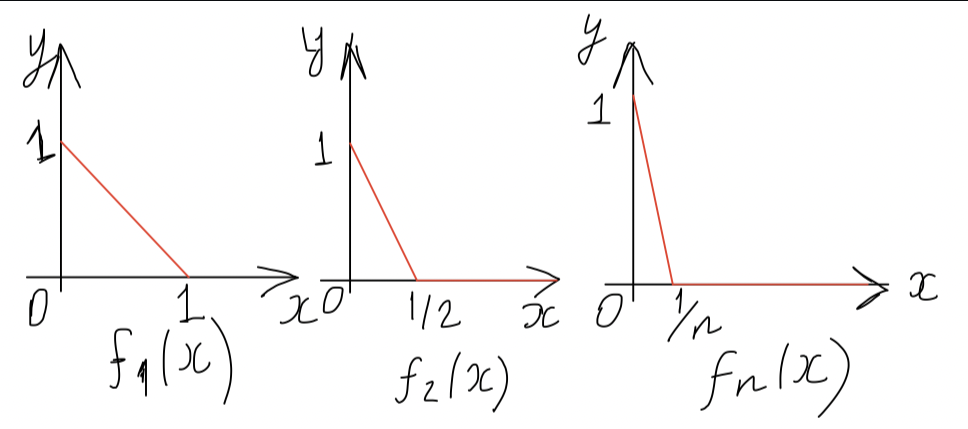
\includegraphics[scale = 0.5]{pictures/10_bilet_primer1.png}
	\end{figure}
	\item
	$1 + \sum\limits_{k=1}^\infty {x^k \over k!}  = 1 + {x\over 1!} + \cdots + {x^n \over n!} + \cdots$ \newline
	$S_{n+1}(x) = 1 + {x\over 1!} + \cdots + {x^n \over n!}$ \newline
	
	$S_{n+1}(x)$ отличается от $e^x$ по формуле Маклорена с остаточным членом в форме Лагранжа на $R_{n+1}(x)= {e^{\theta x}\over {(n+1)!}} x^{n+1}$,  $0 < \theta < 1$
\end{enumerate}
\subsection{Сходимость функциональных рядов и последовательностей в точке и на множестве.}
\underline{\textbf{Определение:}} [сходимость в точке]:\newlineЗафиксируем точку $x_0 \in X$ и рассмотрим числовую последовательность $\{f_n(x_0)\}_{k=1}^\infty$. Если указанная последовательность сходится, то функциональную последовательность $\{f_n(x)\}_{k=1}^\infty$ называют сходящейся в точке $x_0$. \newline \newline
\textbf{Замечание:} аналогичное верно и для функциональных рядов: Если числовой ряд $\sum\limits_{k = 1}^{\infty}  f_k(x_0)$ сходится, то функциональный ряд  $\sum\limits_{k = 1}^{\infty}  f_k(x)$ называют сходящимся в точке $x_0$. \newline
\underline{\textbf{Определение:}} [область сходимости]:\newline
Множество точек в которых сходится функциональная последовательность (или функциональный ряд) называют областью сходимости функциональной последовательности (функционального ряда). \newline 
\textbf{Замечание:} область сходимости функциональной последовательности(ряда) может совпадать с его областью определения $X$, составлять его части или быть $\varnothing$. \newline
\underline{\textbf{Определение:}} [предельная функция]:\newline
Пусть $\widetilde{X} \subset X$ ---  область сходимости функциональной последовательности $\{f_n(x)\}_{k=1}^\infty$, совокупность пределов, взятых в точке $x\in \widetilde{X}$ определяет на $\widetilde{X}$ функцию $y = f(x)$. Эта функция называется предельной функцией $y = f(x) $ функциональной последовательности. \newline
\noindent \underline{\textbf{Определение:}} [сумма ряда]:\newline
Пусть $\widetilde{X} \subset X$ ---  область сходимости функционального ряда  $\sum\limits_{k = 1}^{\infty}  f_k(x)$, совокупность пределов, взятых в точке $x\in \widetilde{X}$ определяет на $\widetilde{X}$ функцию $y = S(x)$. Эта функция называется суммой ряда  $y = S(x) $ функциональной последовательности.\\
\subsection{Понятие равномерной сходимости на множестве.}
\underline{\textbf{Определение:}}[равномерная сходимость функциональной последовательности]:\newline
Функциональная последовательность $\{f_n(x)\}_{n=1}^\infty$ сходится равномерно к функции $y=f(x)$ на множестве $X$ если: \newline \newline
$\forall \varepsilon > 0 $  $\exists N = N(\varepsilon)$: $\forall n \geq N$  $\&$  $\forall x \in X$ $\longmapsto$ $|f_n(x) -f(x)| < \varepsilon$
\newline \newline
\hspace*{5mm} \noindent \textbf{(-):} $\exists \varepsilon_0>0:$ $\forall n$  $\exists n_0 \geq n$  $\&$  $\exists x_n \in X:$ $|f_{n_0}(x_n)-f(x_n)| \geq \varepsilon_0$ 
\newline \newline
\noindent \textbf{Обозначение:} $f_n(x) \overset{x \in X}{\underset{n \rightarrow \infty}{\rightrightarrows}} f(x)$
\noindent \textbf{Примеры:} \newline
1.
\begin{equation*}
	f_n(x) = 
	\begin{cases}
		1-nx &\text{, $0 \leq x \leq {1 \over n}$}\\
		0 &\text{, ${1\over n}< x\leq 1$}
	\end{cases}
\end{equation*}
\begin{equation*}
	f(x) = 
	\begin{cases}
		0 &\text{, $0 < x \leqslant {1}$}\\
		1 &\text{, $x = 0$}
	\end{cases}
\end{equation*}
$\exists \varepsilon_0 = \frac{1}{4}$  $\forall n ~\exists N = n$ $\&$ $\exists x_n = {1\over 2n}: ~|f_n(x_n) - f(x_n)| = \frac{1}{2} > \frac{1}{4} = \varepsilon_0$
$f_n(x)$ сходится неравномерно к $f(x) = 0$ на $[0, 1]$.\\
\noindent 2. $X = [\delta, 1]$\\
\begin{equation*}
	f_n(x) = 
	\begin{cases}
		1-nx &\text{, $\delta \leq x \leq {1 \over n}$}\\
		0 &\text{, ${1\over n}< x\leq 1$}
	\end{cases}
\end{equation*}
Для заданного $\delta > 0$ $\exists N ~\forall n \geq N $ $\longmapsto$ \newline
\hspace*{40 mm} $f_n(x) \equiv 0$ на $[\delta, 1]$ \newline
\hspace*{40 mm} $f(x) \equiv 0$ на $[\delta, 1]$ \newline
Тогда $f_n(x) \overset{x \in [\delta;1]}{\underset{n \rightarrow \infty}{\rightrightarrows}} 0$.\\
\textbf{Замечания:}\newline
\begin{enumerate}
	\item $N$ в определении не зависит от $x$, а только от $\varepsilon$. Один номер для всех $x \in X$ одновременно.
	
	\item Из сходимости функциональной последовательности $\{f_n(x)\}_{n=1}^\infty$ в каждой точке $x \in X$ НЕ следует равномерная сходимость на $X$.
	
\end{enumerate}
\textbf{Замечание:} Если $f_n(x) \overset{x \in X}{\underset{n \rightarrow \infty}{\rightrightarrows}} f(x)$, то 
$f_n(x) \overset{x \in X^/}{\underset{n \rightarrow \infty}{\rightrightarrows}} f(x)$, где $X^/ \subset X$.
\begin{equation*}
	f_n(x) = 
	\begin{cases}
		1-nx &\text{, $\delta \leq x \leq {1 \over n}$}\\
		0 &\text{, ${1\over n}< x\leq 1$}
	\end{cases}
\end{equation*}
\underline{\textbf{Определение:}} [равномерная сходимость функционального ряда]:\newline 
Функциональный ряд $$\sum\limits_{k = 1}^{\infty}  f_k(x)$$ равномерно сходится к $S(x)$ на множестве $X$ , если $S_n(x) \overset{x \in X}{\underset{n \rightarrow \infty}{\rightrightarrows}} S(x)$
\subsection{Критерий Коши равномерной сходимости.}
\underline{\textbf{Теорема [Критерий Коши для функциональной последовательности]:}} Функциональная последовательность $f_n(x) \overset{x \in X}{\underset{n \rightarrow \infty}{\rightrightarrows}} f(x)$ сходится тогда или только тогда, когда выполнено условие Коши
равномерной сходимости функциональной последовательности: \newline
\hspace*{5mm}$\big[\forall \varepsilon > 0 $  $\exists N = N(\varepsilon)$: $\forall n \geq N$  $\&$ $\forall p \in  \mathds{N}$ $\forall x \in X$ $\longmapsto$  $|f_{n+p}(x) -f_n(x)| < \varepsilon\big]$
\noindent \textbf{Доказательство:} \newline
1. \textit{Необходимость $\Rightarrow$:} \newline
\noindent $f_n(x) \overset{x \in X}{\underset{n \rightarrow \infty}{\rightrightarrows}} f(x)$ 
\newline \newline
Тогда: \newline
\hspace*{5mm}$\forall \varepsilon > 0$ $\exists N = N(\varepsilon)$:
$\forall n \geq N$ $\&$ $\forall x \in X$ $\longmapsto$ $|f_n(x) - f(x)| < \varepsilon / 2$ \newline
Тогда и 
\newline 
\hspace*{5mm}$\forall p \in \mathds{N}$ $|f_{n+p}(x) - f(x)| < \varepsilon / 2$
\newline \newline 
Воспользуемся правилом треугольника: \newline \newline
$|f_{n+p}(x) - f_n(x)| \leq |f_{n+p}(x) - f(x)| + |f_n(x) - f(x)| < {\varepsilon \over 2} + {\varepsilon \over 2} = \varepsilon$
\noindent  \newline \newline
2. \textit{Достаточность $\Leftarrow$:} \newline
\hspace*{5mm}$\big[\forall \varepsilon > 0 $  $\exists N = N(\varepsilon)$: $\forall n \geq N$  $\&$ $\forall p \in  \mathds{N}$ $\&$ $\forall x \in X$ $\longmapsto |f_{n+p}(x) -f_n(x)| < \varepsilon\big]$
\newline \newline 
Зафиксируем $x \in X$, тогда $\exists f(x)$ --- предельное значение последовательности $\{f_n(x)\}_{n=1}^\infty$. \newline \newline 
Тогда $f_{n+p}(x) \underset{n \longrightarrow \infty}{\longrightarrow} f(x)$ \newline \newline 
В неравенстве перейдем к предельному при $p \longrightarrow \infty$:\\
$\forall n \geq N$ $\&$ $\forall x \in X$ $\Rightarrow$ $|f_n(x) - f(x)| \leq {\varepsilon \over 2} < \varepsilon$ 
\newline \newline 
Тогда получим, что $f_n(x) \overset{x \in X}{\underset{n \rightarrow \infty}{\rightrightarrows}} f(x)$ по определнию.
\newline \newline 
\noindent \underline{\textbf{Теорема [Критерий Коши для функционального ряда]:}}
Ряд $\sum\limits_{k = 1}^{\infty}  f_k(x) \overset{x \in X}{\rightrightarrows} S(x)$ тогда и только тогда, когда выполнено условие Коши: 
\newline 
\hspace*{5mm}$\big[\forall \varepsilon > 0 $  $\exists N = N(\varepsilon)$: $\forall n \geq N \& $   $\forall p \in  \mathscr{N}~ \&$ $\forall x \in X$ $\longmapsto$ $\left|\sum\limits_{k = n+1}^{n+p}f_k(x)\right| < \varepsilon\big]$
\textbf{Замечание:} критерий Коши для функциональных рядов следует из критерия Коши для функциональных последовательностей, так как: \newline 
$$\left|\sum\limits_{k = n+1}^{n+p} f_k(x)\right| = \left| S_{n+p}(x) - S_n(x)\right|$$
\textbf{Отрицание условия Коши:} 
\newline 
\textit{Для функциональной последовательности:}
\newline
$\exists \varepsilon_0 > 0$: $\forall n$ $\exists n_0 \geq n$ $\& $ $\exists  p_0 \in \mathds{N}$ $\&$ $\exists x_n \in X:$ $|f_{n_0+p_0}(x_n) - f_{n_0}(x_n)| \geq \varepsilon_0$ 
\\[5mm] 
\textit{Для функционального ряда:}
\newline
$\exists \varepsilon_0 > 0$: $\forall n$ $\exists n_0 \geq n ~\&  ~\exists  p_0 \in \mathds{N} ~\& $ $\exists x_n \in X:$ $\left|\sum\limits_{k = n+1}^{n+p}f_k(x_n)\right| \geq \varepsilon_0$ 
\subsection{Критерии равномерной сходимости функциональной последовательности и функционального ряда.}
\underline{\textbf{Теорема 1 [$\sup$-критерий для функциональной последовательности]:}}\newline 
$f_n(x) \overset{x \in X}{\underset{n \rightarrow \infty}{\rightrightarrows}} f(x)$ тогда и только тогда, когда $$\lim\limits_{n \rightarrow \infty} \sup_{x \in X}|f_n(x)-f(x)| = 0$$
\textbf{Доказательство:} 
\newline
Обозначим $M_n = \sup\limits_{x \in X}{|f_n(x)-f(x)|}$. \newline
Тогда запишем  наше равенство в виде: \newline
\hspace*{40mm}$\forall \varepsilon > 0$ $\exists N = N(\varepsilon):$ $\forall n \geq N \mapsto 0 \leq M_n < \varepsilon$ \newline
1. \textit{Необходимость $\Rightarrow$:} \newline

$[f_n(x) \overset{x \in X}{\underset{n \rightarrow \infty}{\rightrightarrows}} f(x)]$ $\stackrel{def}{=}$ $\big[\forall \varepsilon > 0 $  $\exists N = N(\varepsilon)$: $\forall n \geq N$  $\&$  $\forall x \in X$ $\longmapsto$ $|f_n(x) -f(x)| < {\varepsilon \over 2} \big]$
\\[5 mm]
Отсюда, $M_n \leq {\varepsilon \over 2 } < \varepsilon$
\\[ 5 mm]
2. \textit{Достаточность $\Leftarrow$:} \newline
\hspace*{5mm}$\forall x \in X \longmapsto |f_n(x)-f(x)|\leq M_n$ 
\\[ 5 mm]
То есть: \newline
\hspace*{20mm}$\forall \varepsilon > 0$  $\exists N = N(\varepsilon):$  $\forall n \geq N$ $\&$ $\forall x \in X$ $\longmapsto |f_n(x)-f(x)| < \varepsilon$ \newline
\underline{\textbf{Теорема 2 [$\sup$-критерий для функционального ряда]:}}\newline 
Функциональный ряд $\sum\limits_{k = 1}^{\infty}  f_k(x)$ равномерно сходится к $S(x)$ на множестве $X$ тогда и только тогда, когда $$\lim\limits_{n \rightarrow \infty} \sup_{x \in X} |r_n(x)| = 0$$
\textbf{Доказательство:} 
$$r_n(x) = \sum\limits_{k = 1}^{\infty}  f_k(x) -  \sum\limits_{k = 1}^{n}  f_k(x)= \sum\limits_{k = n+1}^{\infty}  f_k(x)$$ \newline
То есть $r_n(x)=S(x)-S_n(x)$ \newline
Но $S_n(x) \overset{x \in X}{\underset{n \rightarrow \infty}{\rightrightarrows}} S(x)$ тогда и только тогда, когда $r_n(x) \overset{x \in X}{\underset{n \rightarrow \infty}{\rightrightarrows}} 0$.\\
\textbf{Примеры:}
1. $f_n(x) = nx^2e^{-nx}$, $x \in [2, +\infty) = X$
$\lim\limits_{n \rightarrow \infty}{nx^2 \over e^{nx}} = 0$ $\Rightarrow$ $y=f(x) \equiv 0$
$f_n'(x) = nx(2-nx)e^{-nx} = 0$
\hspace*{5mm}$x_n = {\frac{2}{n}}$ -- точка максимума, при $x > {\frac{2}{n}}$, $n>1$ $\Rightarrow$ $f'_n(x) < 0$ $\Rightarrow$ $f_n$ убывает на $X$;
$$\sup_{X}f_n(x) \leq f({2\over n}) = {4\over ne^2} \underset{n \rightarrow \infty}{\longrightarrow} 0 $$
Отсюда, $f_n(x) \overset{x \in X}{\underset{n \rightarrow \infty}{\rightrightarrows}} 0$.
2. $f_n(x) = n^2x^2e^{-nx}$, $X = (0,2)$
$$\lim\limits_{n \rightarrow \infty}{n^2x^2 \over e^{nx}} = 0$$ $$\Rightarrow y=f(x) \equiv 0$$
$$f_n'(x) = n^2x(2-nx)e^{-nx} = 0$$
\hspace*{5mm}$x_n = { 2 \over n}$,  $n>1$-- точка максимума. $\Rightarrow$
$$\sup_{X}f_n(x) = {4\over e^2} \underset{n \rightarrow \infty}{\nrightarrow} 0 $$
3. $$f_n(x) = {{\ln(nx)} \over {\sqrt{nx}}} \text{, } X = (0,1)$$
$$\forall n \; \exists n_0 = n \; \& \; \exists p_0 = n \; \& \; \exists x_n = {1 \over n}$$
$$|f_{2n}(x_n) - f_n(x_n)| = \left| {\ln{2}\over{\sqrt{2}}} - {\ln{1}\over{\sqrt{1}}} \right| = {\ln{2}\over{\sqrt{2}}} > \varepsilon_0 = {\ln{2}\over{2\sqrt{2}}}$$
Отсюда, равномерной сходимости нет.
\subsection{Свойства равномерно сходящихся последовательностей и рядов.}
\underline{\textbf{Теорема 1:}} если члены функционального ряда $$\sum\limits_{k = 1}^{\infty}  f_k(x)$$   непрерывны на $[a,b]$ и ряд сходится равномерно на $[a,b]$ к функции $y = S(x)$, то сумма ряда 
$y = S(x)$ непрерывна на $[a,b]$. \\
\textbf{Доказательство:} \newline
$\big[S_n(x) \overset{x \in [a,b]}{\underset{n \rightarrow \infty}{\rightrightarrows}} S(x)\big]\stackrel{def}{=} \big[ \forall \varepsilon > 0 $  $\exists N = N(\varepsilon)$: $\forall n \geq N$  $\&$  $\forall x \in [a,b]$ $\longmapsto$ $|S_n(x) -S(x)| < {\varepsilon \over 3} \big]$
Возьмем $n_0 \geq N$ $\Rightarrow$ $|S_{n_0}(x)-S(x)| < {\varepsilon \over 3}$
При $x_0 \in [a,b]$ выполняется:
$|S_{n_0}(x_0)-S(x_0)| < {\varepsilon \over 3}$
В силу непрерывности $f_k$ на $[a,b]$, $S_{n_0}$ непрерывна на $[a,b]$, в частности в точке $x_0 \in [a,b]$, то есть:
$\forall \varepsilon > 0$ $\exists \delta = \delta(\varepsilon)$: $\forall x \in [a,b]$:  $|x-x_0|<\delta$ $\longmapsto$ $|S_{n_0}(x) - S_{n_0}(x_0)| < {\varepsilon \over 3}$
$\forall x \in [a,b]$: $|x-x_0|<\delta$ $\longmapsto$ 
\newline
$|S(x) - S(x_0)| = \big| [S(x)-S_{n_0}(x)] + [S_{n_0}(x)-S_{n_0}(x_0)] + [S_{n_0}(x_0)-S(x_0)]\big| \leq |S(x)-S_{n_0}(x)| + \big| S_{n_0}(x)-S_{n_0}(x_0)\big| + \big|S_{n_0}(x_0) - S(x_0)\big| < {\varepsilon \over 3} \cdot 3 = \varepsilon$
В силу произвольности выбора точки $x_0 \in [a,b]$ функция $y = S(x)$ непрерывна на $[a,b]$.\\
\underline{\textbf{Теорема 1':}} если члены функциональной последовательности $\{f_n(x)\}_{n=1}^\infty$ в каждой точке $x \in X$  непрерывны на $[a,b]$ и последовательность сходится равномерно на $[a,b]$ к функции $f(x)$, то $y = f(x)$ непрерывна на $[a,b]$. 
\textbf{Замечание:} пусть ряд $$\sum\limits_{k = 1}^{\infty}  f_k(x)$$ удовлетворяет условиям теоремы 1 и $S(x)=\sum\limits_{k = 1}^{\infty}  f_k(x)$.
$$\forall x_0 \in [a,b] \longmapsto \lim\limits_{x\rightarrow x_0} S(x) = S(x_0)$$
Отсюда, $$\lim\limits_{x\rightarrow x_0} \sum\limits_{k = 1}^{\infty}  f_k(x) = \sum\limits_{k = 1}^{\infty}  \lim\limits_{x\rightarrow x_0}f_k(x) $$
При выполнении условий теоремы 1 возможен почленный переход к пределу под знаком суммы для  равномерно сходяшегося функционального ряда, члены которого есть непрерывные функции.\\
\underline{\textbf{Теорема 2:}} если члены функционального ряда $\sum\limits_{k = 1}^{\infty}  f_k(x)$   непрерывны на $[a,b]$ и ряд сходится равномерно на $[a,b]$ к функции $y = S(x)$, то функциональный ряд $\sum\limits_{k = 1}^{\infty}  \int\limits_{a}^{x}f_k(t)dt$ также сходится равномерно на $[a,b]$ к функции $y = \int\limits_{a}^{x}S(t)dt $.\\
\textbf{Доказательство:}
$\sum\limits_{k = 1}^{\infty}  f_k(x)$  сходится равномерно на $[a,b]$ к $y = S(x)$:
$\forall \varepsilon > 0$  $\exists N = N(\varepsilon)$: $\forall n \geqslant N$ $\& $ $\forall x \in [a,b]$ $\longmapsto$ $|S_n(x)-S(x)| < \frac{\varepsilon}{b - a}$
По теореме 1 $S$ непрерывны на $[a,b]$, следовательно $S$ и $f_k $ --- интегрируемые функции ($\forall k$) на $[a,b]$. Обозначим:
$$I(x) = \int\limits_{a}^{x}S(t)dt$$ и $$I_{n}(x) = \sum\limits_{k = 1}^{n}  \int\limits_{a}^{x}f_k(t)dt = \int\limits_{a}^{x}[ \sum\limits_{k = 1}^{n}  f_k(t) ]dt = \int\limits_{a}^x S_n(t)dt$$
$$|I(x)-I_n(x)| = \big|\int\limits_{a}^x[S(t)-S_n(t)]dt\big| \leq \int\limits_{a}^x|S_n(t)-S(t)|dt \leq {\varepsilon \over {b-a}} (x-a) < \varepsilon$$
Итак: 
$\forall \varepsilon > 0 $ $\exists N=N(\varepsilon)$: $\forall n \geq N$  $\&$ $\forall x \in [a,b]$ $\longmapsto |I(x)-I_n(x)| < \varepsilon$, то есть функциональный ряд $$\sum\limits_{k = 1}^{\infty} \int\limits_{a}^{x}f_k(t)dt$$ сходится равномерно на $[a,b]$ к функции $$\int\limits_a^xS(t)dt = \int\limits_{a}^{x}[ \sum\limits_{k = 1}^{\infty}  f_k(t) ]dt$$ и $$\sum\limits_{k = 1}^{\infty}  \int\limits_{a}^{x}f_k(t)dt = \int\limits_{a}^{x}[ \sum\limits_{k = 1}^{\infty}  f_k(t) ]dt$$\\
\underline{\textbf{Теорема 2':}} если члены функциональной последовательности  $\{f_n(x)\}_{n=1}^\infty$ непрерывны на $[a,b]$. и $f_n(x) \overset{[a,b]}{\underset{n \rightarrow \infty}{\rightrightarrows}} f(x)$, то $\int\limits_a^x f_n(t)dt \overset{[a,b]}{\underset{n \rightarrow \infty}{\rightrightarrows}} \int\limits_a^x f(t)dt$.\\
\textbf{Замечания:}
\begin{enumerate}
\item В теоремах 2,2' отрезок $[a,x]$ можно заменить отрезком $[x_0,x] \subset [a,b].$

\item Теоремы 2 и 2' остаются справедливыми, если функции $y=f_k(x)$ интегрируемы на $[a,b]$.
\end{enumerate}
\underline{\textbf{Теорема 3:}} если члены функционального ряда $\sum\limits_{k = 1}^{\infty}  f_k(x)$   непрерывно-дифференцируемы  на $[a,b]$ и функциональный ряд $\sum\limits_{k = 1}^{\infty}  f_k'(x)$ сходится равномерно на $[a,b]$, а числовой ряд $\sum\limits_{k = 1}^{\infty}  f_k(x_0)$ ($x_0 \in [a,b])$ сходится, то функциональный ряд $\sum\limits_{k = 1}^{\infty}  f_k(x)$ сходится равномерно на $[a,b]$ к функции $y = S(x)$ и $S'(x) = \sum\limits_{k = 1}^{\infty}  f_k'(x)$
\textbf{Доказательство:}
Обозначим: $$\widetilde{S}(x)= \sum\limits_{k = 1}^{\infty}  f_k'(x)$$
Из условия теорем 3 и 1 $y = \widetilde{S}(x)$ непрерывна на $[a,b]$.
Ряд $\sum\limits_{k = 1}^{\infty}  f_k'(x)$ можно почленно интегрировать(по теореме 2), то есть:
$$\int\limits_{x_0}^x \widetilde{S}(t)dt = \sum\limits_{k = 1}^{\infty}  \big[\int\limits_{x_0}^{x}f_k'(t)dt\big]$$. \newline
Согласно теореме 2 ряд сходится равномерно на $[a,b]$. 
Но $\int\limits_{x_0}^{x}f_k'(t)dt = f_k(x)-f_k(x_0)$, следовательно: $$\sum\limits_{k = 1}^{\infty}  \big[\int\limits_{x_0}^{x}f_k'(t)dt\big] = \sum\limits_{k=1}^\infty f_k(x)-\sum\limits_{k=1}^\infty f_k(x_0)$$
Ряды слева и справа равномерно-сходящиеся, а значит, $\sum\limits_{k=1}^\infty f_k(x)$ сходится равномерно на $[a,b]$.
$$\int\limits_{x_0}^x \widetilde{S}(t)dt = S(x)-S(x_0)$$
Левая часть -- интеграл с переменным верхним пределом и его производная равна $\widetilde{S}(x)$ $\Rightarrow$ правая часть -- дифференцируемая функция и $S'(x) = \widetilde{S}(x)$, то есть 
$$\bigg(\sum\limits_{k = 1}^{\infty}  f_k(x)\bigg)' = \sum\limits_{k = 1}^{\infty}  f_k'(x)$$
\noindent \textbf{Замечания:}
\begin{enumerate}
\item По условию теоремы 3: $\widetilde{S}(x) = S'(x)$ -- непрерывная функция $\Rightarrow$ $S$ -- непрерывно-дифференцируемая на $[a,b]$.

\item Теорема 3 остается справедливой, если функции $y=f_k(x)$ являются дифференцируемыми функцими.\\
\end{enumerate}
\underline{\textbf{Теорема 3':}} если члены функциональной последовательности $\{f_n(x)\}_{n=1}^\infty$ являются непрерывно-дифференцируемыми функциями на $[a,b]$, числовая последовательность $\{f_n(x_0)\}_{n=1}^\infty$ сходится, где $x_0 \in [a,b]$; а функциональная последовательность $\{f_n'(x)\}_{n=1}^\infty$ равномерно сходится на $[a,b]$, то $\{f_n(x)\}_{n=1}^\infty$ сходится равномерно на $[a,b]$ к функции $y = f(x)$ и справедливо равенство $$f'(x)= \lim\limits_{n\rightarrow \infty} f'_n(x) \text{, }x \in [a,b]$$
\textbf{Замечение:} можно сделать важный вывод: равномерная сходимость не выводит из класса непрерывных функций, а в случае равномерной сходимости производных -- из класса непрерывно дифференцируемых функций.
\subsection{Достаточные признаки сходимости функциональных рядов.}
\underline{\textbf{Теорема 1 [Признак Вейерштрасса]:}}
Если для функционального ряда $$\sum\limits_{k = 1}^{\infty}  f_k(x)$$ можно указать такой числовой ряд с неотрицательными членами $\sum\limits_{k = 1}^{\infty}a_k < \infty$, что $\forall k \geq k_0$ и $\forall x \in X$ выполняется: $0 \leq |f_k(x)| \leq a_k$, то функциональный ряд  $$\sum\limits_{k = 1}^{\infty}  f_k(x)$$ сходится абсолютно и равномерно на $X$.\\
\textbf{Доказательство:}
$$\sum\limits_{k = 1}^{\infty}a_k < \infty \Leftrightarrow \forall \varepsilon > 0 \text{ }\exists N_1 = N_1(\varepsilon)\text{: } \forall n \geq N_1 \text{ }\&\text{ } \forall p \in \mathds{N} \longmapsto \sum\limits_{k = n+1}^{n+p}a_k < \varepsilon$$ 
$$\exists N = max\{N_1, k_0\} \text{ } \Rightarrow \forall n \geq N \text{ } \& \text{ } \forall x \in X \text{ } \& \text{ } \forall p \in \mathds{N}\longmapsto$$ $$\left|\sum\limits_{k = n+1}^{n+p}f_k(x)\right| \leq \sum\limits_{k = n+1}^{n+p}|f_k(x)| \leq \sum\limits_{k = n+1}^{n+p}a_k < \varepsilon$$
\textbf{Следствие:} если сходится числовой ряд $$\sum\limits_{k = 1}^{\infty}a_k,$$ где $a_k = \sup\limits_{x \in X}|f_k(x)|$, то функциональный ряд $\sum\limits_{k = 1}^{\infty}  f_k(x)$ сходится абсолютно и равномерно на $X$. \\
\underline{\textbf{Теорема 2 [Признак Дирихле]:}} Если:
\begin{enumerate}
\item $$\sum\limits_{k = 1}^{\infty}  u_k(x)$$ имеет равномерно ограниченную на $X$ последовательность частичных сумм $\{S_n(x)\}_{n=1}^\infty$: 
\newline

$\exists M > 0 \text{: } \forall x \in X \text{ }\& \text{ } \forall n \in \mathbb{N} \longmapsto |S_n(x)| \leq M$

\item ${\{v_k(x)\}_{k=1}^\infty}$ монотонна на $X$ и равномерно стремится к $0$:
$v_k(x) \leq v_{k+1}(x) \text{ } \forall x \in X \text{} \& \text{ } \forall k$
$[v_k(x) \geq v_{k+1}(x)]$ и $v_k(x) \overset{x \in X}{\underset{k \rightarrow \infty}{\rightrightarrows}} 0$: 

\end{enumerate}
\hspace*{40 mm}то $\sum\limits_{k=1}^{\infty} u_k v_k$ сходится равномерно на $X$.\\
\underline{\textbf{Теорема 2 [Признак Абеля]:}}
Если:
\begin{enumerate}
\item  $\sum\limits_{k=1}^\infty u_k(x)$ равномерно сходится на $X$.

\item ${\{v_k(x)\}_{k=1}^\infty}$ равномерно ограничена и монотонна на $X$.
\end{enumerate}
\hspace*{40 mm}то $\sum\limits_{k=1}^{\infty} u_k v_k$ сходится равномерно на $X$.
%=======================================================================================
%БИЛЕТ 11
%=======================================================================================
\newpage
\section{Билет 11}
\subsection{Степенные ряды с комплексными числами}

\underline{\textbf{Определение:}} $\sum\limits_{k = 0}^\infty c_k(\zeta - a)^k$; $c_k, a \in \mathbb{C} -$ фиксированные числа, $\zeta \in \mathbb{C}$  - переменная.

Такой функциональные ряд называется \textit{степенным}.

$c_k$ - коэф. степенного ряда. Этот ряд сходится в точке а.

$\zeta - a = z \Rightarrow \sum\limits_{k = 0}^\infty c_k z^k$ - будем рассматривать такой степенной ряд, который сходится в т. $z = 0$

\subsection{Теорема 1. [Первая теорема Абеля]}

1. Если степенной ряд $\sum\limits_{k = 0}^\infty c_k z^k$ сходится в т. $z_0 \neq 0$, то он сходится абсолютно в круге: $K_0 = \{z = \mathbb{C}: |z| < |z_0|\}$

2. Если степенной ряд $\sum\limits_{k = 0}^\infty c_k z^k$ расходится в т. $z_1$, то он расходится в любой т. $z: |z| > |z_1|$ 

\begin{figure*}[h!]
\centering
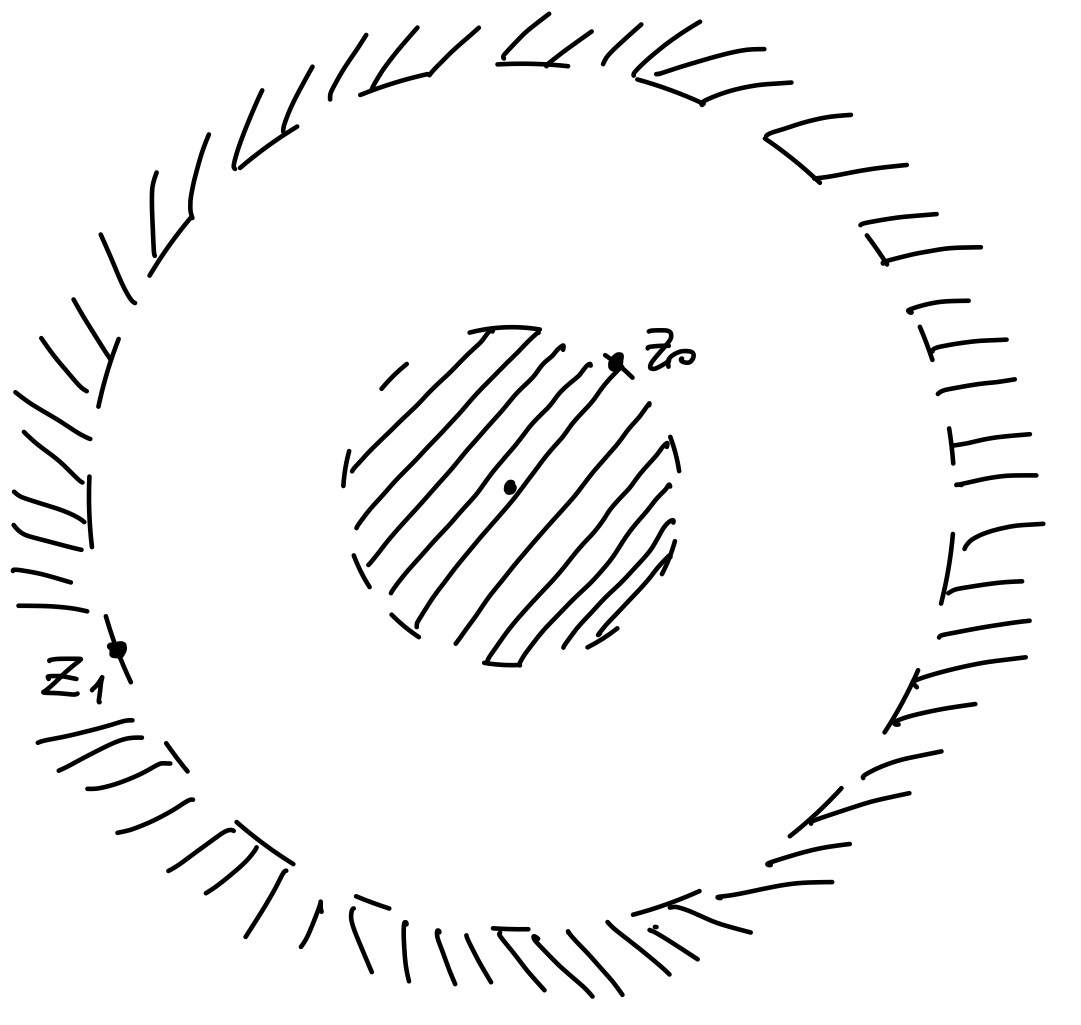
\includegraphics[scale = 0.1]{Que_11_pic_1.jpeg}
\end{figure*}

\textbf{Доказательство:} \\
\ \\
1) $\sum\limits_{k = 0}^\infty c_k z_0^k < \infty \Rightarrow c_k z_0^k \underset{k \to \infty}{\longrightarrow} 0 \Rightarrow \text{Ограничена:} \,  \exists M > 0: \forall k \Rightarrow |c_k z_0^k| \leqslant M$ \\
\ \\
$ \forall z: |z| < |z_0| $ \\
$ |c_k z^k| = | c_k z_0^k  \left(  \frac{z}{z_0} \right)^k | \leqslant M \cdot \left[ q(z) \right]^k, |q(z)| < 1 \Rightarrow \sum\limits_{k = 0}^\infty q^k(z) < \infty \Rightarrow
$\\
$
\Rightarrow \sum\limits_{k = 0}^\infty |c_k z^k| < \infty \Rightarrow \sum\limits_{k = 0}^\infty c_k z^k 
$ cходится абсолютно в точке $z \in K_0$\\
В силу произвольности точки $z \Rightarrow ~ \sum\limits_{k = 0}^\infty c_k z^k$ сходится абсолютно в $K_0$   
\ \\
2) $
\sum\limits_{k = 0}^\infty c_k z_1^k = \infty \Rightarrow \forall z: |z| > |z_1| - \text{ряд} \sum\limits_{k = 0}^\infty c_k z^k \text{ расходится, если бы в точке } z_2: 
$\\
$
|z_2| > |z_1| \text{ ряд } \sum\limits_{k = 0}^\infty c_k z_2^k < \infty \stackrel{1)}{\Rightarrow} \sum\limits_{k = 0}^\infty c_k z_1^k < \infty
$ - противоречие. \\
\textbf{Следствие 1. } Если $\sum\limits_{k = 0}^\infty c_k z_0^k < \infty, z_0 \neq 0$, то $\forall \rho: 0 < \rho < |z_0|$ в круге $K_{\rho} = \{z \in \mathbb{C} : |z| \leqslant \rho \} \text{ ряд } \sum\limits_{k = 0}^\infty c_k z^k$ сходится равномерно. \\
\textbf{Доказательство:} \\
$
\exists M > 0: \forall k \Rightarrow |c_k z_0^k| \leqslant M
$ \\
\ \\
$ \forall z \in K_{\rho} $\\
\ \\
$
|c_k z^k| = |c_k z_0^k \cdot \frac{z^k}{z_0^k} | \leqslant M \left( \frac{\rho}{|z_0|} \right)^k = M \cdot q^k
$ \\
\ \\
$ |q| = \frac{\rho}{|z_0|} < 1 $ ($\frac{\rho}{|z_0|}$ не зависит от $z$), \\
\ \\
$\sum\limits_{k = 0}^\infty q^k < \infty \stackrel{\text{По пр. Вей.}}{\Rightarrow} \sum\limits_{k = 0}^\infty c_k z^k$ сходится равномерно в круге  $K_{\rho}$ \\
\textbf{Следствие 2} Если в т. $z_0 \neq 0 $ выполнено $\sum\limits_{k = 0}^\infty c_k z_0^k < \infty $, то \\
1) $\sum\limits_{k = m}^\infty c_k z^{k - m}$ сходится абсолютно в круге $K_0$ и равномерно в круге $K_{\rho}$ \\
2) $\sum\limits_{k = 1}^\infty k c_k z^{k - 1}$ сходится абсолютно в круге $K_0$ и равномерно в круге $K_{\rho}$ \\
\textbf{Доказательство:} \\
1) $\forall z \in k_0 \Rightarrow |c_k z^{k - m} | = |c_k z_0^k \left(\frac{z}{z_0} \right)^{k - m} \cdot \frac{1}{z_0^m} | \leqslant$ \\
\ \\
$
\frac{M}{|z_0|^m} \cdot | \frac{z}{z_0} |^{k-m} = \frac{M}{|z_0|^m} \cdot q^{k - m} (z), \quad q(z) = |\frac{z}{z0}| < 1
$\\
\ \\
$\sum\limits_{k = m}^\infty q^{k - m} < \infty $ - сходится абсолютно в $K_0$\\
\ \\
$ \forall z \in K_1 \Rightarrow |c_k z^{k - m}| \leqslant \frac{M}{|z_0|^m} \cdot q_1^{k - m}, \quad q_1 = \frac{\rho}{|z_0|} < 1.
$\\
\ \\
$0 < q_1 < 1$ - не зависит от $z$ $\Rightarrow$ по признаку Вейр. в $K_1$ ряд сходится равномерно\\
\noindent2) $\forall z \in K_0$ \\
\ \\
$ |k c_k z^{k-1} | = | \frac{c_k z_0^k}{z_0} \cdot k\left( \frac{z}{z_0} \right)^{k-1} | \leqslant \frac{M}{|z_0|} \cdot  k q^{k - 1}(z), ~q(z) = | \frac{z}{z_0} | < 1 $ \\
\ \\
$ \sum\limits_{k = 1}^\infty k q^k(z) < \infty $ по признаку Даламбера\\
\subsection{Теорема 2. [О радиусе сходимости степенного ряда].}
Для любого степенного ряда существует $R \, \, (R \geqslant 0 \text{ или } R = +\infty)$
такое, что

1) $0 < R < \infty \Rightarrow \sum\limits_{k = 0}^\infty c_k z^k < \infty$ в круге $K = \{ z \in \mathbb{C} : |z| < R\}$ и расходится в $\mathbb{C} \backslash \overline{K}$

2)$R = 0$, то $\sum\limits_{k = 0}^\infty c_k z^k < \infty$ только в $z = 0$

3) $R = +\infty$, то $\sum\limits_{k = 0}^\infty c_k z^k < \infty \  \forall z \in \mathbb{C}$

$R$ - называется радиусом сходимости степенного ряда $\sum\limits_{k = 0}^\infty c_k z^k$

$K$ - круг сходимости.\\
\textbf{Доказательство:} Пусть $\mathscr{D} \subset \mathbb{C}$ - множество сходимости степенного ряда; $\mathscr{D} \neq \varnothing$, т.к. $0 \in \mathscr{D}$

1) $\mathscr{D}$ - огран., $\exists z_0 \in \mathscr{D}, ~z_0 \neq 0$ \\
$R = \underset{z \, \in \, \mathscr{D}}{\sup} |z| $ - сущ. т.к. $\mathscr{D}$ огранич. мн-во.
Докажем: $\forall \  z \in K \Rightarrow  \sum\limits_{k = 0}^\infty c_k z^k < \infty$
$\forall z \in \mathbb{C} \backslash \overline{K} \Rightarrow  \sum\limits_{k = 0}^\infty c_k z^k = \infty$
По определению $\sup \, \forall z'\in K \  \exists z_1 \in \mathscr{D} : |z'| < |z_1| \leqslant R$, т.к.
$ \sum\limits_{k = 0}^\infty c_k z_1^k < \infty \Rightarrow$ 1-я теорема Абеля $ \sum\limits_{k = 0}^\infty c_k (z')^k < \infty$ и сходится абсолютно $\Rightarrow$ В силу произв. $z' \in K \Rightarrow  \sum\limits_{k = 0}^\infty c_k z^k$ сходится абс. в круге $K$
Пусть $z' \notin K \Rightarrow |z'| > R \Rightarrow$ по опред. $\sup z' \notin \mathscr{D} \Rightarrow  \sum\limits_{k = 0}^\infty c_k (z')^k = \infty \Rightarrow$ расходится вне круга $K$
2) $\mathscr{D}$ - огран.;  если $\mathscr{D} = \{0\}$, то ряд сход в т. $z = 0$ и расх в $z \neq 0$
$ \sum\limits_{k = 0}^\infty c_k z^k < \infty \quad z = 0 \quad \Rightarrow R = 0$
3) $\mathscr{D}$ - неогранич. $\Rightarrow \forall z \in \mathbb{C} \  \exists z'  \in \mathscr{D}:$
$|z| < |z'|,  \sum\limits_{k = 0}^\infty c_k (z')^k < \infty \stackrel{\text{1-я т. Аб.}}{\Rightarrow}  \sum\limits_{k = 0}^\infty c_k z^k < \infty$.\\

\subsection{Теорема 3. [Вторая теорема Абеля].}

Если $0<R<+\infty, \  R$ - радиус сходимости $\sum\limits_{k = 0}^\infty c_k z^k$  и $\sum\limits_{k = 0}^\infty c_k R^k < \infty$, то на $[0, R]$ ряд $\sum\limits_{k = 0}^\infty c_k z^k$ сх. равномерно и его сумма $S(x) = \sum\limits_{k = 0}^\infty c_k x^k$ непрерывна $\forall x \in [0, R]$
\textbf{Доказательство:}
$ \sum\limits_{k = 0}^\infty \underbrace{c_k R^k}_{U_k} \cdot \underbrace{\left(\frac{x}{R}\right)^k}_{V_k}$
1) $\sum\limits_{k = 0}^\infty c_k R^k < \infty $
2) $V_k =  \left( \frac{x}{R} \right)^k \quad 0 \leqslant V_k \leqslant 1 \quad \forall x \in [0; R]$
$V_{k + 1} = \left( \frac{x}{R} \right)^{k + 1}  < \left( \frac{x}{R} \right)^k = V_k \quad \forall k$

\hspace*{3 cm}$\Downarrow$ признак Абеля
$\sum\limits_{k = 0}^\infty c_k x^k < \infty$ сходится равномерно на $[0, R]$
$f_k(x) = c_k x^k$  - непрерывна на $[0; R]$\\
$S(x) = \sum\limits_{k = 0}^\infty c_k x^k$ непреревна на $[0; R]$
\subsection{Теорема 4.}
$\sum\limits_{k = 0}^\infty c_k z^k$ 

1) $\lim\limits_{k \to \infty} \sqrt[k]{|c_k|} = \rho \quad (\rho \geqslant 0,\, \rho = +\infty) \Rightarrow R =  \frac{1}{\rho}$
2) Если $|c_k| > 0 \  \forall k \text{ и } \lim\limits_{k \to \infty} \frac{|c_{k+1}|}{|c_k|} = \rho \ (\rho \geqslant 0, \rho = +\infty) \Rightarrow R = \frac{1}{\rho}$.\\
\textbf{Доказательство:}
$K = \{z \in \mathbb{C}: |z| < \frac{1}{\rho} \}$ \\
$z_0 \in K: \sqrt[k]{|c_k z_0^k|} = |z_0| \sqrt[k]{|c_k|} \underset{k \to \infty}{\longrightarrow} |z_0| \cdot \rho < \frac{1}{\rho} \cdot \rho = 1 $

\hspace*{3 cm} $\Downarrow$ По признаку Коши
\hspace*{3 cm}$\sum\limits_{k = 0}^\infty |c_k z_0^k| < \infty$
$z_1: |z_1| > \frac{1}{\rho}$
$\sqrt[k]{|c_k z_1^k|} = |z_1| \sqrt[k]{|c_k|} \underset{k \to \infty}{\longrightarrow} |z_1| \cdot > \frac{1}{\rho} \cdot \rho \Rightarrow
$ По признаку Коши $\sum\limits_{k = 0}^\infty c_k z_1^k = \infty$.\\
\textbf{Пример (показывает, для чего нужна формула Коши-Адамара):}\\
$\sum\limits_{k = 1}^\infty z^{k^2} = z + z^4 + z^9 + z^{16} + z^{25} + .... + z^{k^2} + ...
$
$ \{c_k\} = \{ c_1 = 1, c_2 = c_3 = 0, c_4 = 1, c_5 = c_6 = c_7 = c_8 = 0, c_9 = 1, ... \} $\\
$\overline{\lim\limits_{k \to \infty}} \sqrt[k]{|c_k|} = \lim\limits_{k \to \infty} \sqrt[k^2]{|c_{k^2}|} = 1 \Rightarrow R = 1$.\\ 
\subsection{Теорема 5. [Формула Коши-Адамара].}
Если $R$ - радиус сходимости $\sum\limits_{k = 0}^\infty c_k z^k$, тогда $ R = \frac{1}{\overline{\lim\limits_{k \to \infty}} \sqrt[k]{|c_k|}} $.\\
\textbf{Доказательство:}
1) $ \{ \sqrt[k]{|c_k|}\} $ - неогр.
2) $ \overline{\lim\limits_{k \to \infty} }\sqrt[k]{|c_k|}  = L > 0; \quad L \in R$
3) $ \overline{\lim\limits_{k \to \infty} }\sqrt[k]{|c_k|}  = 0 \Rightarrow \{ \sqrt[k]{|c_k|}\}$ сходится к 0
1) Для бескон. числа номеров $k \in \mathbb{N}$ \\
\indent$|c_k z^k| > 1 \quad \forall z \neq 0, \  z \in \mathbb{C}$ \\
\hspace*{3 cm} $\Downarrow$
Не выполняется необходимое условие сходимости ряда \\
\hspace*{3 cm} $\Downarrow$\\
\hspace*{2 cm} $\sum\limits_{k = 0}^\infty c_k z^k = \infty $\\
\hspace*{3 cm} $\Downarrow$\\
\hspace*{1.9 cm} $\sum\limits_{k = 0}^\infty c_k z^k < \infty \ $ только для $z = 0$
2) Докажем, что
а) $\forall z: |z| < \frac{1}{L}$ ряд сходится
б) $\forall z: |z| > \frac{1}{L}$ ряд расходится
а) $z: \quad |z| < \frac{1}{L}$
Тогда $\exists \, \varepsilon > 0: |z| < \frac{1}{L + \varepsilon} < \frac{1}{L} $\\
$\varepsilon > 0 \  \exists \, k_0(\varepsilon): \forall k \geqslant k_0 \Rightarrow \sqrt[k]{|c_k|} < L + \frac{\varepsilon}{2}
$ \\
$ \sqrt[k]{|c_k z^k|} = |z| \sqrt[k]{|c_k|} \leqslant \frac{L + \frac{\varepsilon}{2}}{L + \varepsilon}
$\\
$\Downarrow$ По признаку Коши
$\sum\limits_{k = 0}^\infty c_k z^k < \infty \ $ в круге $K = \{z: |z| < \frac{1}{L}\}$
б) $\forall z: |z| > \frac{1}{L} \Rightarrow \exists \, \varepsilon > 0: |z| > \frac{1}{L - \varepsilon} > \frac{1}{L} $
$[\   \exists \  \{c_{k_n}\} : \lim\limits_{n \to \infty} \sqrt[k_n]{|c_{k_n}|} = L \,] \stackrel{\text{def}}{=} [\varepsilon > 0 \  \exists \, n_0 : \forall n \geqslant n_0 \mapsto L - \varepsilon < \sqrt[k_n]{|c_{k_n}|} < L + \varepsilon \,]$ 
$\sqrt[k_n]{|c_{k_n}| z^{k_n}} = |z| \sqrt[k_n]{|c_{k_n}|} > \frac{1}{L - \varepsilon} \cdot (L - \varepsilon) = 1 \quad \forall n \geqslant n_0  \Rightarrow |c_{k_n} z^{k_n}| > 1 \Rightarrow$
$\Rightarrow$ Не выполняется необходимых условий сходимости \\
\hspace*{3 cm} $\Downarrow$
Ряд расходится $\forall z: |z| > \frac{1}{L}$
3) $\overline{\lim\limits_{k \to \infty} }\sqrt[k]{|c_k|} = 0 \Rightarrow \{ \sqrt[k]{|c_k|}\}$ сходится к 0.\\
$\forall z \in \mathbb{C}, \   z \neq 0 : \frac{1}{2|z|} = \varepsilon: \quad  \exists \, k_0(\varepsilon) : \forall k \geqslant k_0 \Rightarrow \sqrt[k]{|c_k|} < \frac{1}{2|z|} \Rightarrow$
$\Rightarrow \sqrt[k]{|c_k|\cdot |z^k|} = |z|\sqrt[k]{|c_k|} < |z| \cdot \frac{1}{2|z|} = \frac{1}{2} < 1$ 

\hspace*{1 cm} $\Downarrow$ По признаку Коши

$\sum\limits_{k = 0}^\infty c_k z^k  < \infty \quad \forall z \in \mathbb{C}$

\subsection{Теорема 6.}
Для рядов \\
$\sum\limits_{k = 0}^\infty c_k z^k, \quad \quad \sum\limits_{k = 0}^\infty \frac{c_k z^{k + 1}}{k + 1}, \quad \quad \sum\limits_{k = 0}^\infty k c_k z^{k - 1} \quad$

\hspace*{0.5 cm}1) \hspace*{2.4 cm}2)\hspace*{2.7 cm}3)\\
радиус сходимости один и тот же.

1) $R_1, K_1$

2) $R_2, K_2$

3) $R_3, K_3$

Надо доказать: $R_1 = R_2 = R_3 = R$.\\
\textbf{Доказательство:}
$\forall k \in \mathbb{N} \Rightarrow \frac{1}{k + 1} < 1 \leqslant k$

$|\frac{c_k}{k + 1} z^{k + 1}| \leqslant |z| \cdot |c_k z^k| \leqslant |z|^2 \cdot |k c_k z^{k - 1}|$
$\underbrace{ |z| \cdot |c_k z^k| \leqslant |z|^2 \cdot |k c_k z^{k - 1}|}_{1)} \quad \quad \underbrace{|\frac{c_k}{k + 1} z^{k + 1}| \leqslant |z| \cdot |c_k z^k|}_{2)}$

1) $\forall z \neq 0 \in K_3 \Rightarrow \sum\limits_{k = 0}^\infty c_k z^k < \infty \Rightarrow R_1 \geqslant R_3$

2) $\forall z \neq 0 \in K_1 \Rightarrow \sum\limits_{k = 0}^\infty \frac{c_k}{k + 1} z^{k+1} < \infty \Rightarrow R_1 \leqslant R_2$

В результате: $R_3 \leqslant R_1 \leqslant R_2 $
Надо доказать, что $R_2 \leqslant R_3$
$z \in K_2 \ \  \exists \, \rho < R_2: z \in K_{\rho} \quad |k c_k z^{k - 1}| = |k c_k z^{k - 1} \cdot \frac{k + 1}{k + 1} \cdot \frac{z^2}{z^2}|$ = 
$|\frac{c_k}{k + 1} \cdot z^{k + 1} \cdot \frac{k(k+1)}{z^2}| = | \frac{c_k}{k + 1} \cdot \rho^{k + 1} \cdot \frac{k(k + 1)}{z^2} \cdot \left( \frac{z}{\rho} \right)^{k + 1}| \stackrel{\exists M > 0}{\leqslant} $

$\leqslant \frac{M}{|z|^2} k(k+1) q_1^{k + 1}, \text{ где } |q_1| < 1 \quad q_1 = \frac{z}{\rho}$

\hspace*{3 cm} $\Downarrow$
$\forall z \in K_2 \Rightarrow \sum\limits_{k = 0}^\infty k c_k z^{k - 1} < \infty \Rightarrow R_3 \geqslant R_2$

Тогда в сумме $R_1 = R_2 = R_3 = R$

%=======================================================================================
%БИЛЕТ 12
%=======================================================================================
\newpage
\section{Билет 12}
\subsection{Степенные ряды с действительными членами.}
\underline{\textbf{Теорема:}}. Если $R$ -- радиус сходимости степенного ряда и выполнено следующее:
\begin{equation*}
\Large \displaystyle \sum\limits_{k = 0}^{\infty} a_k(x-a)^k = f(x),\ x\in (a - R, a + R),\ x,~a_k,~a \in \mathbb{R}
\end{equation*}
то
\begin{enumerate}
\item $f$ бесконечно дифференцируемая функция на $(a-R,~a+R)$ и  выполняется: 
\begin{equation*}
	\Large \displaystyle f^{(m)}(x) = \sum\limits_{k = m}^{+\infty} k(k-1)\dots (k - (m-1))a_k(x-a)^{k-m}
\end{equation*}
\item $\Large \displaystyle \forall\ x \in (a - R, a + R) \mapsto \int\limits_{a}^{x} f(t)dt = \sum\limits_{k = 0}^{\infty} \frac{a_k}{k+1}(x-a)^{k+1}$ 
\end{enumerate} 
\textbf{Доказательство:}
$\forall \rho: 0 < \rho < R  \text{ на } [a - \rho; a + \rho ]$ равномерная сходимость $\Rightarrow$ всё можно делать.\\
\textbf{Следствие}. $a_n = \cfrac{f^{(k)}(a)}{k!}$
\subsection{Бесконечная дифференцируемость суммы степенного ряда на интервале сходимости.}
Покажем, что сумма степенного ряда дифференцируема в интервале сходимости.
\underline{\textbf{Теорема:}}. Сумма степенного ряда $f(x)=\sum\limits_{n=0}^{\infty} c_{n}\left(x-x_{0}\right)^{n}$ дuфференцируема в интервале сходимости и производная равна
\begin{equation*}
f^{\prime}(x)=\sum\limits_{n=1}^{\infty} n c_{n}\left(x-x_{0}\right)^{n-1},
\end{equation*}
причём ряды $\sum\limits_{n=1}^{\infty} n c_{n}\left(x-x_{0}\right)^{n-1}$ и $\sum\limits_{n=0}^{\infty} c_{n}\left(x-x_{0}\right)^{n}$ имеют одинаковый радиус сxoдимости.
\textbf{Доказательство}. Члены ряда $c_{n}\left(x-x_{0}\right)^{n}$ являются непрерывно дифференцируемыми на всей числовой прямой функциями. Пусть $R=\cfrac{1}{\varlimsup\limits_{n \rightarrow \infty} \sqrt[n]{\left|c_{n}\right|}}$ радиус сходимости ряда $\sum\limits_{n=0}^{\infty} c_{n}\left(x-x_{0}\right)^{n}$ и точка $x$ принадлежит интервалу сходимости $\left(x_{0}-R, x_{0}+R\right) .$ Тогда существует отрезок $[a, b] \subset\left(x_{0}-R, x_{0}+R\right)$, включающий точку $x .$
Рассмотрим ряд $\sum\limits_{n=1}^{\infty} n c_{n}\left(x-x_{0}\right)^{n-1}$, полученный почленным дифференцированием ряда $\sum\limits_{n=0}^{\infty} c_{n}\left(x-x_{0}\right)^{n} .$ Вычислим его радиус сходимости $R^{\prime}$
\begin{equation*}
R^{\prime}=\frac{1}{\varlimsup \limits_{n \rightarrow \infty} \sqrt[n-1]{\left|n c_{n}\right|}} = \frac{1}{\varlimsup \limits_{n \rightarrow \infty} \sqrt[n-1]{\left|c_{n}\right|}\cdot \sqrt[n-1]{n}} = \frac{1}{\varlimsup \limits_{n \rightarrow \infty}(\left|c_{n}\right|^{\frac{1}{n}})^{\frac{n}{n-1}}}=R
\end{equation*}
Таким образом, ряды $\sum\limits_{n=1}^{\infty} n c_{n}\left(x-x_{0}\right)^{n-1}$ и $\sum\limits_{n=0}^{\infty} c_{n}\left(x-x_{0}\right)^{n}$ имеют одинаковый интервал сходимости, и, следовательно, на отрезке $[a, b]$ ряд $\sum\limits_{n=1}^{\infty} n c_{n}\left(x-x_{0}\right)^{n-1}$ сходится равномерно. По теореме о дифференцируемости суммы функционального ряда сумма степенного ряда $f(x)$ дифференцируема в точке $x$ и верна формула
\begin{equation*}
f^{\prime}(x)=\sum\limits_{n=1}^{\infty} n c_{n}\left(x-x_{0}\right)^{n-1}
\end{equation*}
что полностью доказывает теорему. $\square$
Теперь в силу доказанной теоремы при дифференцировании суммы степенного ряда вновь получаем степенной ряд с тем же радиусом сходимости. Это позволяет нам сформулировать
следующую теорему:
\underline{\textbf{Теорема:}}. Сумма степенного ряда $f(x)=\sum\limits_{n=0}^{\infty} c_{n}\left(x-x_{0}\right)^{n}$ дuффepeнцируема любое количество раз и верна формула
\begin{equation*}
f^{(k)}(x)=\sum\limits_{n=k}^{\infty} c_{n} n(n-1)(n-2) \ldots(n-k+1)\left(x-x_{0}\right)^{n-k}
\end{equation*}
причём радиусы сходимости всех получающихся рядов одинаковы.
\textbf{Доказательство}. По предыдущей теореме функция $f(x)=\sum\limits_{n=0}^{\infty} c_{n}\left(x-x_{0}\right)^{n}$ дифференцируема и $f^{\prime}(x)=\sum\limits_{n=1}^{\infty} n c_{n}\left(x-x_{0}\right)^{n-1}$, причём радиусы сходимости обоих рядов совпадают. Далее, пусть существует
\begin{equation*}
f^{(k-1)}(x)=\sum\limits_{n=k-1}^{\infty} c_{n} n(n-1)(n-2) \ldots(n-k+2)\left(x-x_{0}\right)^{n-k+1}
\end{equation*}
Применяя к функции $f^{(k-1)}(x)$ предыдущую теорему, получаем, что $f^{(k-1)}(x)$ дифференцируема и верна формула
\begin{equation*}
f^{(k)}(x)=\left(f^{(k-1)}(x)\right)^{\prime}=\sum\limits_{n=k}^{\infty} c_{n} n(n-1)(n-2) \ldots(n-k+2)(n-k+1)\left(x-x_{0}\right)^{n-k},
\end{equation*}
причём радиусы сходимости рядов для $f^{(k-1)}(x)$ и $f^{(k)}(x)$ совпадают. Тем самым, следуя методу математической индукции, полностью доказывает эту теорему. $\square$
\subsection{Единственность представления функции степенным рядом.}
\underline{\textbf{Определение:}} Регулярная функция.
Пусть в каждой точке $z \in \mathbb{E}$, где $\mathbb{E}$ -- множество точек комплексной плоскости, поставлено в соответствие комплексное число $\omega$. На множестве $\mathbb{E}$ определена функция комплексного переменного, $\omega = f(z)$.
Если $\forall \epsilon > 0\ \exists \ \sigma = \sigma_{\epsilon} > 0:\ \forall z\ :\ |z - a| < \sigma_{\epsilon} \longmapsto |f(z) - f(a)| < \epsilon$, то функцию $f(z)$ называют непрерывной в точке а.
И , наконец, Функция комплексного переменного $f(z)$ называется регулярной в точке $a$, если она определена в некоторой окрестности точки $a$ и представима в некотором круге $|z - a| < \rho$, $\rho > 0$, сходящимся к $f(z)$ степенным рядом $f(z) = \sum\limits_{n = 0}^{\infty} c_n(z-a)^n\ \ $ (*).\\
\underline{\textbf{Теорема [Единственность представления функции степенным рядом]:}}
Функция $f(z)$, регулярная в точке $a$, единственным образом представляется рядом (*).\\
\textbf{Доказательство}. Пусть функция $f(z)$ имеет два представления в виде степенного ряда в круге $K = \{z: |z-a|<\rho\}$, где $\rho > 0$, т.е.
\begin{equation*}
f(z) = \sum\limits_{n = 0}^{\infty}c_n(z-a)^n = \sum\limits_{n = 0}^{\infty}\widetilde{c_n}(z-a)^n\ \ (**)
\end{equation*}
Теперь покажем, что $c_n = \widetilde{c_n} \ $, для $n = 0, 1, 2,\dots$
По условию ряды $\sum\limits_{n = 0}^{\infty}c_n(z-a)^n$ и $\sum\limits_{n = 0}^{\infty}\widetilde{c_n}(z-a)^n$ сходятся в круге $K$, и поэтому эти ряды сходятся равномерно в круге $K_1 = \{z: |z - a|\leqslant \rho_1 < \rho \}$, а их общая сумма -- непрерывная в круге $K_1$ функция. В частности, функция $f(z)$ непрерывна в точке $a$. Подходя к пределу при $z \to a$ в равенстве (**), получаем $c_0 = \widetilde{c_0}$. Отбрасывая одинаковые слагаемые $c_0$ и $\widetilde{c_0}$ в равенстве (**), получаем после деления на $(z - a)$ равенство:
\begin{equation*}
c_1 + c_2(z - a) + c_3(z - a)^2 +\ \dots = \widetilde{c_1} + \widetilde{c_2}(z - a) + \widetilde{c_3}(z - a)^2 +\ \dots\ ,
\end{equation*}
которое справедливо в круге $K$ с выколотой точкой $a$. Ряды в левой и правой части сходятся равномерно в круге $K_1$. Переходя в равенстве к пределу при $z \to a$, получаем $c_1 = \widetilde{c_1}$. Справедливость равенства $c_n = \widetilde{c_n}$ при любой $n \in \mathbb(N)$ устанавливается при помощи индукции.
\subsection{Достаточные условия разложимости бесконечно дифференцируемой функции в степенной ряд}
\underline{\textbf{Теорема [Достаточные условия сходимости ряда Тейлора к функции]:}} 
Если $f$ бесконечно дифференцируемая функция на ($a - \delta , a + \delta$), $\delta > 0$ и $\exists M > 0 : \forall x \in (a - \delta, a + \delta) \mapsto |f^{(k)}(x)| \leqslant M\ ,\ k = 0,1,\dots \ $, то ряд Тейлора сходится к функции $f(x)$ в каждой точке $x$ нашего интервала:
\begin{equation*}
\Large \displaystyle f(x) =f(a) + \sum\limits_{k = 1}^{\infty} \frac{f^{(k)}(a)}{k!}(x-a)^k\ ,\ \forall x\in (a - \delta, a + \delta)
\end{equation*}
\textbf{Доказательство}. Достаточные условия разложимости бесконечно дифференцируемой функции в степенной ряд.
\begin{equation*}
\begin{gathered}
	\mathbf{r}_n(x) = \frac{f^{(n+1)}(\xi)}{(n+1)!}(x-a)^{n+1}\ ,\ \text{где } \xi \text{ между } x \text{ и } a  \\
	|\mathbf{r}_n(x)| \leqslant M\cdot \frac{|x - a|^{n+1}}{(n+1)!}\\
	\text{т.к.  }|x - a|\ \geqslant 0 \Rightarrow \lim\limits_{k \to \infty} \frac{|x - a|^k}{k!} = 0\ ,\ \text{тогда справедливо следующее:}\\
	\forall x \in (a - \delta, a + \delta)\ \ \forall n\in \mathbb{N} \longmapsto |\mathbf{r}_n(x)| 	\leqslant M \cdot \frac{\mid x - a\mid^{n+1}}{(n + 1)!} \underset{n \rightarrow \infty} \longrightarrow 0\ \ \ \square\ .
\end{gathered}
\end{equation*}
\subsection{Ряд Тейлора}
Пусть функция $f$ -- бесконечно дифференцируема в точке $a$ (т.е в этой точке у функции $f$ существует производная любого порядка), тогда
\underline{\textbf{Определение:}}. Рядом Тейлора функции $f$ в точке $a$ называется следующее выражение:
\begin{equation*}
f(a) + \sum\limits_{k = 1}^{\infty} \frac{f^{(k)}(a)}{k!}(x-a)^k 
\end{equation*}
\textbf{Замечание}. Если функция регулярна в точке $a$, то она раскладывается в степенной ряд и этот степенной ряд и есть ряд Тейлора, однако не все функции раскладываются в степенной ряд, поэтому справедливо следующее выражение:
\begin{equation*}
f(x) \neq f(a) + \sum\limits_{k = 1}^{\infty} \frac{f^{(k)}(a)}{k!}(x-a)^k 
\end{equation*}
\textbf{Пример}. Рассмотрим следующую функцию:
\begin{equation*}
f(x) = \begin{cases}
	e^{-\frac{1}{x^2}}\ ,\ x \neq 0;\\
	0\ ,\ x = 0\ .
\end{cases}
\end{equation*}
Эта функция непрерывная в нуле. Найдем ее производные:
\begin{equation*}
f^{\text{'}}(x) = \frac{2}{x^3}\cdot e^{-\frac{1}{x^2}}\\
\end{equation*}
\begin{equation*}
f^{\text{''}}(x) = \left[ \left( \frac{2}{x^3}\right)^2 - \frac{6}{x^4} \right]\cdot e^{-\frac{1}{x^2}}\\
\end{equation*}
\begin{equation*}
f^{\text{'''}}(x) = \left[ \left( \frac{2}{x^3}\right)^3 - \frac{12}{x^7} - \frac{2^4}{x^4} + \frac{24}{x^5} \right]\cdot e^{-\frac{1}{x^2}}\\
\end{equation*}
Таким образом $f^{\text{(m)}}(x) = Q_{3m}(\frac{1}{x})\cdot e^{-\frac{1}{x^2}}$, где $Q_{3m}(\frac{1}{x})$ -- многочлен степени $3m$ от $\frac{1}{x}$. Тогда понятно, что 
\begin{equation*}
\lim\limits_{x\to 0} \frac{e^{-\frac{1}{x^2}}}{x^k} = 0 \Rightarrow 
\end{equation*}
\begin{equation*}
\Rightarrow f^{\text{(m)}}(x) = \begin{cases}
	Q_{3m}(\frac{1}{x}) \cdot e^{-\frac{1}{x^2}}\ ,\ x \neq 0;\\
	0\ ,\ x = 0\ .
\end{cases}
\end{equation*}
Тогда $\forall x \neq a$ ряд Тейлора будет представлять собой нулевой ряд, хотя сама функция не нулевая $\Rightarrow f(x) \neq f(a) + \sum\limits_{k = 1}^{\infty} \frac{f^{(k)}(a)}{k!}(x-a)^k.\ \square$ 
\subsection{Формула Тейлора с остаточным членом в интегральной форме.}
Функция $f$ -- бесконечно дифференцируема в некоторой окрестности точки $a$, тогда этой функции соответствует некоторый ряд: 
\begin{equation*}
\Large \displaystyle f(a) + \sum\limits_{k = 1}^{\infty} \frac{f^{(k)}(a)}{k!}(x-a)^k
\end{equation*}
\textbf{Обозначение}. $\Large \displaystyle P_n(x) = f(a) + \sum\limits_{k = 1}^{n} \frac{f^{(k)}(a)}{k!}(x-a)^k$ -- $n$-ая частичная суммма ряда Тейлора (многочлен Тейлора).
Тогда, если $\mathbf{r}_n(x) = f(x) - P_n(x) \underset{n \rightarrow \infty} \longrightarrow 0$, то это означает, что ряд Тейлора сходится к функции $f$ в точке $x$:
\begin{equation*}
\Large \displaystyle f(x) = f(a) + \sum\limits_{k = 1}^{\infty} \frac{f^{(k)}(a)}{k!}(x-a)^k
\end{equation*}
\underline{\textbf{Теорема:}}. Если $f^{(n+1)}$ непрерывна на $(a - \delta, a + \delta),\ \delta > 0$, то:
\begin{enumerate}
\item $\Large \displaystyle \mathbf{r}_n(x) = \frac{1}{n!} \int\limits_{a}^{x} (x - t)^nf^{(n+1)}(t)dt$, т.е. её остаточный член на этом интервале представим в интегральной форме.
\item $\Large \displaystyle \mathbf{r}_n(x) = \frac{f^{(n+1)}(\xi)}{(n+1)!}(x-a)^{n+1}$
\end{enumerate}
\textbf{Доказательство}. 
\begin{enumerate}
\item Доказательство будем проводить при помощи мат. индукции:
\begin{enumerate}
	\item Мы знаем, что $\Large \displaystyle f(x) - f(a) = \int\limits_{a}^{x} f^{'}(t)dt$. Тогда:
	\begin{equation*}
		\begin{cases}
			u = f^{'}(t)\ ,\ dv = dt\\
			du = f^{''}(t)dt\ ,\ v = -(x-t), \text{ x - это константа}
		\end{cases}
	\end{equation*}
	получаем, что $\Large \displaystyle f(x) - f(a) = -f^{'}(t)(x-t) \bigg|_a^x + \int\limits_a^x (x-t) f^{''}(t)dt = $\\
	$\Large \displaystyle = f^{'}(a)(x-a) + \frac{1}{1!} \int\limits_a^x (x-t) f^{''}(t)dt \Rightarrow$\\
	$\Rightarrow \Large \displaystyle  f(x) = f(a) + \frac{f^{'}(a)}{1!}(x-a) + \frac{1}{1!} \int\limits_a^x (x-t) f^{''}(t)dt$.\\
	Получили при $n = 1$ остаточный член в интегральной форме (получена база индукции).
	\item Предположим, что при $n - 1$ верно, тогда найдем для $n$ :
	\begin{equation*}
		\Large \displaystyle f(x) = f(a) + \sum\limits_{k = 1}^{n - 1} \frac{f^{(k)}(a)}{k!}(x-a)^k + \frac{1}{(n-1)!}\int\limits_a^x (x-t)^{n - 1} f^{(n)}(t)dt
	\end{equation*}
	Тогда:
	\begin{equation*}
		\begin{cases}
			u = f^{n}(t)\ ,\ dv = (x-t)^{n-1}dt\\
			du = f^{n + 1}(t)dt\ ,\ v = -\frac{(x-t)^n}{n}
		\end{cases}
	\end{equation*}
	получаем, что $\Large \displaystyle f(x) = f(a)\ +\ \sum\limits_{k = 1}^{n - 1} \frac{f^{(k)}(a)}{k!}(x-a)^k\ -\ \frac{(x-t)^n f^{(n)}(t)}{n!} \bigg|_a^x +\ \frac{1}{n!} \int\limits_a^x (x-t)^n f^{(n+1)}(t)dt$. Тогда получаем, что:
	\begin{equation*}
		\Large \displaystyle f(x) = f(a)\ +\ \sum\limits_{k = 1}^{n} \frac{f^{(k)}(a)}{k!}(x-a)^k + \frac{1}{n!} \int\limits_a^x (x-t)^n f^{(n+1)}(t)dt \ \square
	\end{equation*}
	
\end{enumerate}
\item Это просто остаточный член в форме Лагранжа (доказывалось в прошлом семестре).
\end{enumerate}
%=======================================================================================
%БИЛЕТ 13
%=======================================================================================
\section{Билет 13}
\subsection{Разложение в ряд Тейлора основных элементарных функций: $e^x$, $\cos x$, $\sin x$, $\ln (1 + x)$, $(1 + x)^{\alpha}$.}
\subsubsection*{1. Показательная и гиперболические функции.}
\begin{center}
$y = e^x, \; x \in \mathbb{R}$
\vspace{8pt}
$x \in (-\rho, \, \rho), \; \rho > 0$
\end{center}
Поскольку $(e^x)^{(k)} = e^x $, то $0 < f(x) < e^{\rho}$ и $0 < f(x)^{(k)} < e^{\rho}$. Ряд Тейлора функции $y = e^x$ сходится к ней на $( - \rho, \, \rho)$ по теореме о достаточном условии представимости функции её рядом Тейлора.
$\forall \rho > 0 \Rightarrow R = + \infty$
\[ e^x = \ryad \frac{x^k}{k!}\]
\[y = \sh x, \; y = \ch x, \; x \in \mathbb{R} \]
\[ \sh x = \frac{e^x - e^{-x}}{2}, \; \ch x = \frac{e^x + e^{-x}}{2} \]
\[ \sh x = \ryad \frac{x^{2k + 1}}{(2k + 1)!} \,, \; \ch x = \ryad \frac{x^{2k}}{(2k)!}, \; R = +\infty\]
\subsubsection*{2. Тригонометрические фунции.}
\begin{center}
$y = \sin x, \; y = \cos x, \; x \in \mathbb{R}$
\vspace{8pt}
$| f^{(k)} (x) | \le 1$, $\forall k = 0, \, 1, \, 2, \, \ldots$
\end{center}

$$ 
\sin x = \ryad \frac{(-1)^k x^{2k + 1}}{(2k + 1)!}, \; \cos x = \ryad \frac{(-1)^k x^{2k}}{(2k)!}, \;R = + \infty
$$
\subsubsection*{3. Степенная функция.}
$$y = (1 + x)^{\alpha}, \; \alpha \in \mathbb{R}$$
1) $\alpha = 0, \; y = 1$
2) $\alpha = n, \; n \in \mathbb{N}, \; f(x) = \ryad C^k_n x^k$ - бином Ньютона
3) $\alpha$ - произвольное, $\alpha \in \mathbb{R}$
$$ 
f^{(n + 1)}(x) = \alpha (\alpha - 1) \ldots (\alpha - n) (1 + x)^{\alpha - (n + 1)} $$
$$
\mathrm{r}_n(x) = \frac{\alpha(\alpha - 1) \ldots (\alpha - n)}{n!} \int\limits_0^x \left(\frac{x - t}{1 + t} \right)^n (1 + t)^{\alpha - 1} dt
$$
Пусть $t = x \tau$, $0 \leqslant \tau \leqslant 1$, тогда $dt = x d \tau$
$$
\mathrm{r}_n(x) =  \frac{\alpha(\alpha - 1) \ldots (\alpha - n)}{n!} x^{n + 1} \int\limits_0^1 \left( \frac{1 - \tau}{1 + x\tau} \right)^n ( 1 + x \tau)^{\alpha - 1} d \tau
$$
Пусть $|x| < 1$, тогда $|1 + \tau x| \geqslant 1 - \tau$
\begin{equation*}
(1+x \tau)^{\alpha-1} \leqslant \beta(x)=
\begin{cases}
	(1+|x|)^{\alpha-1}, & \alpha \geq 1 \\
	(1-|x|), & \alpha<1
\end{cases}
\end{equation*}
$ | \alpha | \leqslant m $, $m \in \mathbb{N}$. Тогда $\forall n > m$
\begin{multline*}
\left| \frac{\alpha(\alpha - 1) \ldots (\alpha - n)}{n!} \right| \leqslant \frac{m (m + 1) \ldots (m + n)}{n!} \leqslant \frac{(m + n)!}{n!} = \\
= (n + 1)(n + 2) \ldots (n + m)\leqslant (2n)^m
\end{multline*}
В итоге
$$ 
\left| \mathrm{r}_n (x) \right| \leqslant 2^m \beta (x) |x| \cfrac{n^m}{\left(\cfrac{1}{|x|}\right)^n} \xrightarrow{n \rightarrow + \infty} 0
$$
Так как 
$$
a = \frac{1}{|x|} > 1 \hspace{0.5cm} \lim\limits_{n \rightarrow + \infty} \frac{n^m}{a^n} = 0$$
Следовательно 
$$
(1 + x)^{\alpha} = \ryad C_{\alpha}^k x^k, \; C_{\alpha}^k = \frac{\alpha (\alpha - 1) \ldots (\alpha - (k -1))}{k!}, \; |x| < 1, \; R = 1 
$$
\underline{В частности:}
$$
\frac{1}{1 - x} = \ryad x^k, \; \frac{1}{1 + x} = \ryad (-1)^k x^k, \; |x| < 1
$$
\subsubsection*{4. Логарифмические функции.}
$$
y = \ln(1 - x), \; y' = - \frac{1}{1 - x} = - \ryad x^k
$$
$$
y = \ln(1 + x), \; y' = - \frac{1}{1 + x} = \ryad (-1)^k x^k
$$
Раскладываем в интервалах сходимости каждую функцию в ряд Тейлора, а потом почленно интегрируем, и помним, что при почленном интегрировании радиус сходимости не меняется. 
$$ 
y = \ln(1 - x) = - \ryad \frac{x^{k + 1}}{k + 1} = - \sum\limits^{\infty}_{k = 1} \frac{x^k}{k}, \; |x| < 1
$$
$$
y = \ln(1 + x) = \ryad \frac{(-1)^k x^{k + 1}}{k + 1} = - \sum\limits^{\infty}_{k = 1} \frac{(-1)^{k - 1} x^k}{k}, \; |x| < 1
$$
\subsubsection*{5. Обратные тригонометрические функции.}
Обратные тригонометрические функции можно разложить в ряд Тейлора, сначала продифференцировав и воспользовавшись известными результатами.
\subsection{Разложение в степенной ряд комплекснозначной функции $e^z$.}
\textbf{Докажем, что} 
$$
e^z = \ryad \frac{z^k}{k!}, \; R = + \infty
$$
$$
\cos z = \ryad \frac{(-1)^k z^{2k}}{(2k)!}, \;\; \sin z = \ryad \frac{(-1)^k z^{2k + 1}}{(2k + 1)!}, \;\;\; R = + \infty
$$
\textbf{Доказательство:}
Так как $z = x + iy$ и по формуле Эйлера: $e^{i \varphi} = \cos(\varphi) + i \sin(\varphi)$, то 
$$
e^z = e^{x + iy} = e^x \left( \cos y + i \sin y \right)
$$
$$
e^x = \ryad \frac{x^k}{k!}, \; \cos y = \ryad (-1)^k \frac{y^{2k}}{(2k)!}, \; \sin y = \ryad (-1)^k \frac{y^{2k + 1}}{(2k + 1)!}
$$
\begin{multline*}
e^{iy} = cos y + i \sin y = \ryad (-1)^k \frac{y^{2k}}{(2k)!} + i \ryad (-1)^k \frac{y^{2k + 1}}{(2k + 1)!} =  \\ = \ryad \frac{(iy)^{2k}}{(2k)!} + \ryad \frac{(iy)^{2k + 1}}{(2k + 1)!} = \ryad \frac{(iy)^{k}}{k!} = e^{iy}
\end{multline*}
$$
e^z = \ryad \frac{x^k}{k!} \cdot \ryad \frac{(iy)^{k}}{k!}
$$
Докажем, что
$$
\ryad \frac{(z_1 + z_2)^k}{k!} = \ryad \frac{z_1^k}{k!} \cdot \ryad \frac{z_2^k}{k!}
$$
\begin{multline*}
\ryad \frac{(z_1 + z_2)^k}{k!} = \ryad \frac{1}{k!} \cdot \sum\limits_{j = 0}^k C_k^j z_1^j z_2^{k - j} = \ryad  \sum\limits_{j = 0}^k \frac{1}{k!} \cdot \frac{k!}{j! \cdot (k - j)!} z_1^j z_2^{k - j} = \\ = \ryad  \sum\limits_{j = 0}^k \frac{z_1^j}{j!} \cdot \frac{z_2^{k - j}}{(k - j)!} = \frac{z_1^0}{0!} \cdot \frac{z_2^0}{0!} + \left(\frac{z_1^0}{0!} \cdot \frac{z_2^1}{1!} + \frac{z_1^1}{1!} \cdot \frac{z_2^0}{0!} \right) + \\ + \left( \frac{z_1^0}{0!} \cdot \frac{z_2^2}{2!} + \frac{z_1^1}{1!} \cdot \frac{z_2^1}{1!} + \frac{z_1^2}{2!} \cdot \frac{z_2^0}{0!} \right) + \ldots
\end{multline*}
Это можно проиллюстрировать следующим образом:
\begin{table}[h!]
\centering
\resizebox{0.6\textwidth}{!}{%
	\begin{tabular}{|c|c|c|c|c|c|}
		\hline
		& $u_0$      & $u_1$      & $u_2$      & $u_3$ & ... \\ \hline
		$v_0$ & $u_0 \cdot v_0$ & $u_1 \cdot v_0$ & $u_2 \cdot v_0$ & ...  &     \\ \hline
		$v_1$ & $u_0 \cdot v_1$ & $u_1 \cdot v_0$ & ...       &      &     \\ \hline
		$v_2$ & $u_0 \cdot v_2$ & ...       &           &      &     \\ \hline
		$v_3$ & ...       &           &           &      &     \\ \hline
		...  &           &           &           &      &     \\ \hline
	\end{tabular}%
}
\end{table}
Мы обходим таблицу по диагоналям, так что сумма индексов элементов была константа для каждой группы слагаемых. Тогда действительно:
$$
\ryad \frac{(z_1 + z_2)^k}{k!} = \ryad  \sum\limits_{j = 0}^k \frac{z_1^j}{j!} \cdot \frac{z_2^{k - j}}{(k - j)!} = \ryad \frac{z_1^k}{k!} \cdot \ryad \frac{z_2^k}{k!}
$$
Тогда по доказанной выше лемме:
$$
e^z = \ryad \frac{x^k}{k!} \cdot \ryad \frac{(iy)^k}{k!} = \ryad \frac{(x + iy)^k}{k!} = \ryad \frac{z^k}{k!}
$$
Теперь 
\begin{multline*}
e^{iz} = \ryad \frac{(iz)^k}{k!} = \ryad \frac{(iz)^{2k}}{(2k)!} + \ryad \frac{(iz)^{2k + 1}}{(2k + 1)!} = \\ = \ryad (-1)^k \frac{z^{2k}}{(2k)!} + i \ryad (-1)^k \frac{z^{2k + 1}}{(2k + 1)!}
\end{multline*}
\begin{multline*}
e^{-iz} = \ryad \frac{(-iz)^k}{k!} = \ryad \frac{(-iz)^{2k}}{(2k)!} + \ryad \frac{(-iz)^{2k + 1}}{(2k + 1)!} = \\ = \ryad (-1)^k \frac{z^{2k}}{(2k)!} - i \ryad (-1)^k \frac{z^{2k + 1}}{(2k + 1)!}
\end{multline*}
$$
\frac{e^{iz} + e^{-iz}}{2} = \cos z = \ryad (-1)^k \frac{z^{2k}}{(2k)!}
$$
$$
\frac{e^{iz} - e^{-iz}}{2} = \sin z = \ryad (-1)^k \frac{z^{2k + 1}}{(2k + 1)!}
$$
\textbf{Что и требовалось доказать.}
%======================================================================================
\newpage 
 \section{Анализ функции} 
Теперь можно перейти к анализу заданной функции: 
\begin{equation}
 f(x) = \ln {({x} + {{1}})}\end{equation}
Значение функции в точке $x_0 = 0$:  $f(x_0) = 0$ \\ 
\subsection{Касательная к графику функции в точке} 
 Уравнение касательной к графику функции в точке $x_0 = 0$:\[ y = 1 \cdot x + (0)\]
\subsection{Производная 3-ой степени} 
 Из предисловия нетрудно заметить, что 
\begin{eqnarray}
 f^{(1)}(x) =  \frac {{1}}{({x} + {{1}})}\end{eqnarray}\\
\begin{eqnarray}
 f^{(2)}(x) =  \frac {{(-1)}}{({({x} + {{1}})} ^ {{2}})}\end{eqnarray}\\
\\...Следующую часть простейших преобразований оставляем читателю...\\\\После небольшого количества элементарных преобразований получаем:\\ 
\begin{eqnarray} 
f^{(3)} =  \frac {({{0}} - {({{(-1)}} \cdot {({{2}} \cdot {({x} + {{1}})})})})}{({({({x} + {{1}})} ^ {{2}})} ^ {{2}})}\end{eqnarray} 
\\В точке $x_0 = 0$:  $f^{(3)}(x_0) = 2$
\subsection{Разложение по формуле Тейлора} 
 Разложим функцию по формуле Тейлора в точке $0$ до $x^{4}$: 
\begin{eqnarray}
f(x) = \ln {({x} + {{1}})} = 0 + \frac{1}{1} \cdot (x)^{1}\nonumber\\ 
 - \frac{1}{2} \cdot (x)^{2} + \frac{2}{6} \cdot (x)^{3} - \frac{6}{24} \cdot (x)^{4}\nonumber\\ 
 + o((x)^{4})\end{eqnarray}
\subsection{График функции} 
 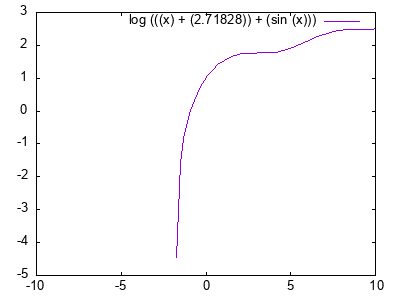
\includegraphics{graphic.png}\\

\newpage 
 \section{Подсчет погрешности} 
 Подсчитаем погрешность величины f: \\
\[ f = {({x} + {({y} ^ {{2}})})} - {z}\]
Для значений величин: \\$x = 5$, $\delta_{x} = 0.01$\\$y = 2$, $\delta_{y} = 0.02$\\$z = 3$, $\delta_{z} = 0.03$\\\[\delta_{f} = \sqrt{((1) \cdot 0.01)^2 + ((4) \cdot 0.02)^2 + ((-1) \cdot 0.03)^2} = 0.0860233 \]
\end{document}
